
\documentclass[11pt]{article}

\usepackage[utf8]{inputenc}
\usepackage[T1]{fontenc}
\usepackage{lmodern}
\usepackage{amsmath,amssymb,amsfonts}
\usepackage{graphicx}
\usepackage{booktabs}
\usepackage{caption}
\usepackage{subcaption}
\usepackage{makecell}
\usepackage{booktabs}
\usepackage{algorithm}
\usepackage{algpseudocode}


\usepackage{tikz}
\usetikzlibrary{arrows.meta}
\usepackage{xcolor}
\definecolor{origincolor}{RGB}{72, 175, 130}
\definecolor{destcolor}{RGB}{210, 90, 70}
\definecolor{intcolor}{RGB}{150, 150, 150}
\definecolor{auxcolor}{RGB}{180, 180, 180}
\definecolor{crossgreen}{RGB}{29, 158, 117}
\definecolor{crosspurple}{RGB}{120, 100, 200}
\definecolor{crossyellow}{RGB}{200, 140, 0}
\DeclareMathOperator*{\argmax}{arg\,max}


\DeclareMathOperator*{\argmin}{arg\,min}

\usepackage{geometry}
\geometry{margin=1in}

\usepackage{setspace}
\onehalfspacing

\usepackage{hyperref}
\hypersetup{
    colorlinks=true,
    linkcolor=blue,
    citecolor=blue,
    urlcolor=blue
}

\usepackage[
    backend=biber,
    style=authoryear,
    sorting=ynt
]{biblatex}
\addbibresource{sample.bib}


\title{Graph Multi-Output Gaussian Processes for Origin-Destination Matrix Calibration via Bayesian Optimization}



\author{Inès Ben Hamza}
\date{June 2026}

\begin{document}

\begin{titlepage}
    \centering
    \vspace*{1cm}
    \includegraphics[width=0.45\textwidth]{hec-montreal-vector-logo.png}
    \vspace{2cm}
    
    {\Large\bfseries
    Graph Multi-Output Gaussian Processes for Origin-Destination Matrix Calibration via Bayesian Optimization
    \par}
    
    \vspace{1.5cm}
    {\large Inès Ben Hamza \par}
    \vspace{1cm}
    {\normalsize
    HEC Montréal\\
    Department of Decision Sciences
    \par}
    
    \vfill
    {\normalsize
    \textit{Supervised project for the attainment of \\
     the Master of Science degree (M.Sc.)}
    \par}
    
    \vspace{1cm}
    {\normalsize Supervisor: Osorio Carolina \par}
    \vspace{1.5cm}
    {\normalsize July 2026 \par}
\end{titlepage}

\tableofcontents
\newpage

\section{Introduction}

Origin-Destination (OD) demand estimation is a foundational problem in transportation planning. The OD matrix, encoding trip volumes between zone pairs over a given time period, is rarely directly observable and must instead be inferred from link-level traffic counts collected by loop sensors. 

Recovering a demand vector consistent with observed 
counts requires repeated evaluation of a traffic simulation model, making the problem expensive, noisy, and effectively black-box. This computational bottleneck severely constrains the number of candidate solutions that can be explored, and motivates the use of surrogate-based optimization methods that approximate the objective function to guide 
search efficiently under limited simulation budgets.

Bayesian Optimization (BO) has emerged as a principled and sample-efficient framework for expensive black-box problems, maintaining a Gaussian Process (GP) surrogate over the objective landscape and selecting new candidates by 
maximizing an acquisition function that balances exploration and exploitation. Recent work has demonstrated the potential of BO for 
simulation-based transportation problems including signal 
control~\parencite{tay2021bayesian}, 
network 
design~\parencite{yin2022bobb}, and OD 
calibration~\parencite{huo2023simulation}.


Existing BO formulations for OD calibration, however, aggregate
network-wide discrepancy into a scalar objective, collapsing the vector of per-edge flow residuals into a single value before any surrogate is fitted.
This aggregation discards structure that is physically meaningful: flows on different edges are not independent, as they are coupled through shared demand and network topology. Forcing the surrogate to relearn these
dependencies from data alone reduces sample efficiency precisely where it
matters most, and ignores prior knowledge about the road network that is
already available before any simulation is run.

\paragraph{Research question.}
Does replacing the scalar GP surrogate in Bayesian optimization for OD
calibration with a multi-output GP, one that explicitly encodes inter-edge
dependencies through either a learned coregionalization matrix (ICM) or a
graph-structured kernel derived from road network topology, improve sample
efficiency and calibration accuracy over simpler per-edge and scalar baselines?
And if so, under what conditions, in terms of network size, route-overlap
density, and simulation budget, does the added complexity pay off?

We address this limitation by replacing the scalar GP surrogate with a Multi-Output Gaussian Process (MOGP) that jointly models per-edge flow residuals and explicitly captures their statistical dependencies. We adopt the Intrinsic Coregionalization Model (ICM), in which the cross-output covariance is parameterized as a learned low-rank coregionalization matrix, and consider graph-structured task kernels derived from the road network topology as a structured alternative, so that edges sharing junctions or lying on the same corridor are encouraged to share statistical strength through the surrogate. As an ablation, we also fit Independent GPs (IndGP), one per edge residual, without any cross-output sharing: any gain of ICM or the graph-structured kernels over IndGP is therefore attributable specifically to the modelled cross-output dependencies, not merely to the move from a scalar to a per-edge objective. All four surrogate variants — scalar GP, IndGP, ICM, and graph-structured kernels — are embedded within a standard BO loop using Expected Improvement as the acquisition function and evaluated on synthetic SUMO benchmarks with known ground-truth OD demand, enabling a controlled comparison of calibration accuracy, convergence speed, and sample efficiency. A central finding is that the independent GP baseline is surprisingly competitive: fitting inter-task covariance does not consistently improve over independent per-edge models at the simulation budgets studied, a result we analyse in detail in Section~\ref{sec:discussion}.


The remainder of the paper is organized as follows. Section~\ref{sec:litreview} reviews related work on OD calibration and surrogate-based optimization. Section~\ref{sec:prelim} introduces the mathematical background. Section~\ref{sec:method} formulates the calibration problem and describes the four surrogate families. Section~\ref{sec:experiments} presents the experimental setup and results. Section~\ref{sec:discussion} discusses the findings, limitations, and directions for future work. Section~\ref{sec:conclusion} concludes.


\subsection{Origin--Destination Calibration in Traffic Networks}


Origin–Destination (OD) matrix estimation is a fundamental problem in transportation network modelling. OD matrices encode the travel demand between all pairs of zones and, through network assignment models, determine the resulting link flows. Early foundational methodologies relied on single-level statistical estimation frameworks, assuming fixed, congestion-independent route choice proportions. Notably, \textcite{maher1983inferences} introduced a Bayesian inference approach, while \textcite{cascetta1984estimation} formalized the Generalized Least Squares (GLS) estimator.
These formulations, however, implicitly assume fixed route proportions, which becomes untenable in congested networks where route choices evolve dynamically with traffic volumes. To address this, classical congested OD calibration is cast as a bilevel optimisation problem: the upper level minimises a goodness-of-fit objective relative to observed counts, while the lower level solves a traffic assignment problem to ensure behavioural equilibrium. \textcite{yang1992estimation} explicitly formalised this as a bilevel programming framework under user equilibrium conditions, while \textcite{spiess1990gradient} developed gradient-based solution heuristics to tackle its computational complexity.
While effective in analytical settings, these gradient-based methods rely on the differentiability of the demand-to-flow mapping which is an assumption that breaks down when microscopic simulators are used. Simulators such as SUMO incorporate stochastic driver behaviour and event-driven dynamics, making the input–output mapping from OD demand to simulated flows non-differentiable and analytically intractable.



Simulation-based calibration methods address this limitation by treating the
simulator as an expensive black-box function. One line of work constructs
computationally tractable surrogate models that approximate the simulator
response using a limited number of simulation evaluations
\parencite{osorio2013simulation, osorio2015computationally}. For instance,
\textcite{osorio2013simulation} propose a simulation-based optimization
framework that combines a quadratic polynomial approximation with an
analytical queueing network model, thereby exploiting structural properties of
traffic dynamics to guide the search toward improved solutions under tight
simulation budgets.




An alternative approach embeds calibration directly within the simulation loop, without constructing an explicit surrogate. \textcite{flotterod2011bayesian} propose a Bayesian calibration framework for agent-based traffic simulations that iteratively updates agents' plan choice distributions using observed traffic counts. The method performs calibration through successive simulation iterations and Bayesian updates, using an analytical linearization to efficiently incorporate the observed traffic counts.


However, both approaches face limitations. Analytical metamodels rely on
problem-specific modeling assumptions and substantial domain knowledge, which
can limit their transferability across networks and applications. 

In contrast, simulation-embedded approaches may require many simulator evaluations because they update the calibration through repeated simulation iterations without learning a global surrogate model to guide the search.


These challenges have motivated the development of data-driven probabilistic
surrogates, particularly Gaussian-process-based methods, which offer flexible
function approximation together with principled uncertainty quantification.


In this work, we adopt the surrogate-based paradigm and model the simulator response using a Gaussian Process within a Bayesian Optimization framework. Unlike classical gradient-based OD calibration methods, which rely on analytical sensitivity information, and simulation-embedded approaches, our formulation learns a probabilistic surrogate of the simulator response to guide the sequential selection of simulation evaluations. 

The GP posterior provides principled uncertainty estimates, enabling an effective balance between exploration and exploitation for sample-efficient calibration under a limited simulation budget~\parencite{snoek2012practical,frazier2018tutorial}.


Such approaches have been successfully applied to traffic simulation calibration, including the calibration of vehicle speed parameters in microscopic simulators, where a Bayesian Optimization-based calibration framework achieved faster convergence and greater robustness than SPSA-based calibration methods~\parencite{shi2025traffic}

More generally, Bayesian Optimization has been successfully applied to the calibration of a wide range of transportation simulation models, including Origin--Destination demand calibration and large-scale activity-based travel demand models~\parencite{schultz2018bayesian,agriesti2023bayesian}.







\subsection{Graph-Based Kernels}
\label{sec:litreview_graphkernels}

In network settings, the physical topology provides a natural inductive
bias: adjacent edges share junctions and are physically coupled through
traffic flow dynamics, so their residuals can be expected to covary.
Graph-based kernels incorporate this structure directly into the covariance
function by defining similarity through functions of the graph Laplacian,
whose spectral decomposition captures the geometry of the underlying
network.

\textcite{kondor2002diffusion} introduced the diffusion kernel, which
models a heat-diffusion process on the graph and is defined as the matrix
exponential
\[
    K = \exp(-\beta L),
\]
where $L$ denotes the graph Laplacian and $\beta > 0$ controls the extent
of diffusion.

Building on this idea, \textcite{smola2003kernels} proposed a general
regularization framework for graph kernels in which smoothness is enforced
through the quadratic form
\[
    \langle f, r(L)f \rangle,
\]
where $r(\cdot)$ is a monotonically increasing function of the Laplacian
eigenvalues. The regularized Laplacian corresponds to the particular choice
$r(\lambda)=1+\sigma^2\lambda$. Writing
\[
    f = \sum_i \beta_i v_i,
\]
where $\{v_i\}$ are the eigenvectors of $L$, yields
\[
    \langle f, r(L)f \rangle
    =
    \sum_i \beta_i^2\, r(\lambda_i).
\]


This formulation penalizes graph components associated with large Laplacian
eigenvalues more strongly than those associated with small eigenvalues,
thereby favoring functions that vary smoothly over the graph. The
corresponding kernel is the Green's function of the regularization operator
and, for the regularized Laplacian, is given by
\[
    K = (I+\sigma^2L)^{-1}.
\]





More recently, \textcite{borovitskiy2021matern} introduced a Matérn family
of graph kernels via a stochastic PDE formulation, extending the Matérn
construction from Euclidean and Riemannian domains to graphs while
retaining a tunable smoothness parameter. Like diffusion and regularized
Laplacian kernels, these kernels are defined spectrally through the graph
Laplacian and encode smoothness with respect to the graph topology.


Complementary approaches incorporate graph structure directly within Gaussian process models through Laplacian-based regularization. In particular, \textcite{venkitaraman2020gaussian} propose Gaussian processes over graphs that enforce smoothness with respect to the graph Laplacian, improving predictive performance when training data are scarce.


In the transportation domain specifically, graph-structured models 
have been applied to both traffic forecasting and speed prediction. 
\textcite{li2018dcrnn} and \textcite{yu2018stgcn}  propose DCRNN and STGCN, respectively, two influential deep learning architectures for traffic forecasting that jointly model spatial and temporal dependencies on graph-structured traffic networks. While both achieve strong predictive performance, they are not inherently designed to provide the probabilistic uncertainty estimates required by Bayesian Optimization.

 
 Within the GP framework, 
\textcite{le2017local} develop local Gaussian processes for fine-grained 
traffic speed prediction by leveraging additive kernels to encode directed 
road network topology and incorporate side information such as segment 
length and betweenness centrality. More recently, \textcite{maddix2022dgamgp} 
propose the Directed Graph Advection Matérn Gaussian Process (DGAMGP), 
which encodes the dynamics of the graph advection operator directly into the 
Matérn kernel of a GP, enabling principled uncertainty quantification of 
traffic flow on directed graphs. 



Crucially, however, neither of these GP-based approaches is designed for simulation-based calibration. Both focus on predicting or interpolating observed traffic states, whereas our objective is to construct GP surrogates within a Bayesian Optimization framework to recover latent demand parameters from simulator outputs.



\subsection{Bayesian Optimization}


Bayesian Optimization (BO) is a strategy for optimizing expensive black-box functions by through sequential evaluations. Rather than relying on gradient information, BO constructs a probabilistic surrogate of the objective function to guide the search toward promising regions while limiting the number of costly evaluations. This has made it a powerful tool in applications such as the accelerated discovery of high-performance alloys \parencite{xue2016accelerated}, chemical reaction optimization \parencite{shields2021bayesian}, deep learning hyperparameter tuning \parencite{snoek2012practical}, and the calibration of large-scale transportation simulation models \parencite{agriesti2023bayesian}.

The framework combines two core components: a probabilistic surrogate model that approximates the unknown objective, and an acquisition function that determines where to sample next by balancing exploration of uncertain regions with exploitation of promising ones \parencite{shahriari2016}.

The surrogate model is typically a Gaussian Process (GP), whose properties and kernel choices are discussed in detail in  Section~\ref{sec:prelim}. Within the Bayesian Optimization framework, the GP posterior provides both a predictive mean and predictive uncertainty (variance) at unsampled points, which are directly exploited by the acquisition function to determine where to evaluate next \parencite{garnett2023bayesian}.

Three widely used acquisition functions are Probability of Improvement (PI) \parencite{kushner1964}, Expected Improvement (EI) \parencite{mockus1978}, and the GP Upper Confidence Bound (GP-UCB) \parencite{srinivas2010}. EI is particularly popular due to its its ability to balance exploration and exploitation through the predictive mean and variance \parencite{shahriari2016}. 


Expected Improvement (EI) selects the next evaluation point by maximizing the expected gain relative to the best objective value observed so far. For a minimization problem, the improvement at a candidate point is defined as the positive reduction relative to the current best objective value, and EI computes its expectation under the Gaussian Process posterior. As a result, EI naturally favors candidate points that either improve upon the current best predicted objective value or exhibit high predictive uncertainty, thereby achieving a principled balance between exploitation and exploration. In simulation-based calibration settings, where each function evaluation is computationally expensive, this property makes EI particularly effective as it prioritizes evaluations that are most likely to yield meaningful improvements.

Formally, in the case of noiseless observations, the expected improvement at a candidate point $\mathbf{x}$ can be written as
\[
\alpha_{\text{EI}}(\mathbf{x}) = \mathbb{E}\big[ \max(f^* - f(\mathbf{x}), 0) \big],
\]
where $f^*$ denotes the best (lowest) objective value observed so far.
\label{sec:ei}
Under a Gaussian Process posterior, this expectation admits a closed-form expression\parencite{garnett2023bayesian}.


While the concept of EI was established by \textcite{mockus1978}, it was \textcite{jones1998ego} who popularized it through the Efficient Global Optimization (EGO) algorithm, which maximizes EI exactly via a branch-and-bound procedure and incorporates rigorous model validation diagnostics to ensure surrogate quality.

A key limitation of analytic acquisition functions such as EI is that their closed-form
expressions rely on the posterior over the objective being Gaussian. This assumption holds
when the objective is a linear functional of the GP outputs, as in the scalar and
independent-GP surrogates considered here, but fails when the objective is a nonlinear
transformation of a jointly Gaussian posterior, such as the sum of squared residuals. In
such settings, Monte Carlo (MC) acquisition functions provide a principled alternative:
the expectation is estimated by averaging the improvement over samples drawn from the
joint GP posterior. These samples are generated using the reparameterization trick, in
which a posterior sample is expressed as a deterministic transformation of Gaussian noise,
allowing gradients to propagate through the Monte Carlo estimate
\parencite{Wilson2018,Balandat2020}. \textcite{Balandat2020} introduce the BoTorch
library, which implements \texttt{qExpectedImprovement} (\texttt{qEI}) using
this approach, enabling gradient-based optimization of the acquisition function.


In transportation applications, Bayesian Optimization has been successfully applied to simulation-based calibration problems, where simulator evaluations are computationally expensive and gradient information is unavailable \textcite{agriesti2023bayesian,schultz2018bayesian}. \textcite{schultz2018bayesian} demonstrate this by formulating the calibration of transportation simulation models as a black-box optimization problem. Their framework employs a Gaussian Process surrogate together with the Expected Improvement acquisition function to iteratively calibrate origin--destination demand through an Evaluation--Integration--Exploration loop. Motivated by the high computational cost of transportation simulator evaluations, the proposed approach seeks to improve sample efficiency by minimizing the number of simulator runs required to identify well-calibrated solutions. In contrast, \textcite{chen2020} exploit the internal structure of an activity-based model system to derive approximate analytical gradients through microsimulation. Their stochastic gradient-based calibration procedure achieves greater computational efficiency, stability, and convergence than state-of-the-art simulation-based optimization methods, but requires access to simulator internals and structural assumptions that are unavailable in fully black-box settings. Consequently, Bayesian Optimization remains particularly attractive when reliable gradient information is unavailable or impractical to obtain, as is often the case for complex transportation simulators such as SUMO.


A recurring challenge in simulation-based calibration is the mismatch between the multi-dimensional nature of simulator outputs and the scalar objective assumed by standard Bayesian Optimization (BO) acquisition functions. A single SUMO evaluation yields link flows across all monitored edges simultaneously, yet acquisition functions such as Expected Improvement (EI) are traditionally defined for scalar-valued objectives \parencite{shahriari2016}. The literature addresses this tension through two principal approaches.

The first strategy consists of aggregating multiple outputs into a single scalar objective before surrogate modeling. This is typically achieved through a composite calibration score that combines several performance metrics into a single quantity to be optimized. \textcite{agriesti2023bayesian} illustrate this approach by combining OD matrix error, modal share discrepancy, and worker coverage into a unified calibration objective. While straightforward to implement, this strategy commits to a fixed aggregation scheme from the outset and discards potentially informative correlation structures among simulator outputs that the surrogate could otherwise exploit.

The second approach defers aggregation until after surrogate modeling by representing simulator outputs jointly through a multi-output Gaussian Process (MOGP), which explicitly captures inter-output dependencies \parencite{alvarez2012kernels, liu2018}. Rather than aggregating outputs prior to modeling, a scalar objective can be constructed from the joint predictive distribution once the surrogate has been fitted. For example, one may define a weighted objective $S(\mathbf{x}) = \mathbf{w}^\top \mathbf{e}(\mathbf{x})$, where uncertainty is propagated through the full inter-task covariance structure. This preserves compatibility with standard acquisition functions while allowing the optimization procedure to exploit correlations among outputs. The resulting uncertainty representation is generally richer, but comes at the cost of increased model complexity and computational overhead.

The trade-off between simplicity and computational efficiency on the one hand, and richer uncertainty quantification on the other, motivates the modeling choice adopted in this work, described in Section~\ref{sec:method}.




\bigskip

Together, these results establish that Gaussian Process surrogate models combined with Bayesian Optimization provide an effective framework for calibrating expensive simulation models, and that multi-output Gaussian 
Processes and graph-based kernels offer a principled way to exploit the structured dependencies inherent to traffic networks. Before detailing the proposed methodology, we introduce the mathematical background 
underlying these components in the following section.


\section{Preliminaries}
\label{sec:prelim}


\subsection{Gaussian Processes}
\label{sec:prelim_gp}


Gaussian Processes (GPs) are nonparametric probabilistic models that 
define a distribution over functions: any finite collection of function 
values evaluated at inputs $\mathbf{x}_1, \ldots, \mathbf{x}_n$ follows 
a multivariate Gaussian distribution. A GP is fully characterised by a 
mean function $m(\mathbf{x})$ and a covariance (kernel) function 
$k(\mathbf{x}, \mathbf{x}')$~\parencite{rasmussen2006gaussian}.

Given a set of $n$ noisy observations $\mathbf{y} = f(\mathbf{X}) + 
\boldsymbol{\varepsilon}$ with $\boldsymbol{\varepsilon} \sim 
\mathcal{N}(\mathbf{0}, \sigma^2_n \mathbf{I})$, the GP posterior at a 
new input $\mathbf{x}_*$ is Gaussian with mean and variance
\begin{align*}
\mu(\mathbf{x}_*) &= \mathbf{k}_*^\top 
    (\mathbf{K} + \sigma^2_n \mathbf{I})^{-1} \mathbf{y}, \\
\sigma^2(\mathbf{x}_*) &= k(\mathbf{x}_*, \mathbf{x}_*) - 
    \mathbf{k}_*^\top (\mathbf{K} + \sigma^2_n \mathbf{I})^{-1} 
    \mathbf{k}_*,
\end{align*}
where $\mathbf{K} \in \mathbb{R}^{n \times n}$ is the kernel matrix with
$K_{ij} = k(\mathbf{x}_i, \mathbf{x}_j)$, and
$\mathbf{k}_* \in \mathbb{R}^{n}$ is the vector of covariances between the
test input $\mathbf{x}_*$ and the training inputs,
\[
\mathbf{k}_* =
\left[
k(\mathbf{x}_1,\mathbf{x}_*),
\ldots,
k(\mathbf{x}_n,\mathbf{x}_*)
\right]^\top.
\]

Their effectiveness stems from two core strengths: the principled quantification and propagation of uncertainty, and the flexible incorporation of structural prior knowledge about the target function. Crucially, both the predictive mean and variance are available in closed form, making GPs particularly attractive for sequential decision-making, where these uncertainty estimates can be directly exploited by acquisition functions in Bayesian optimisation~\parencite{frazier2018tutorial}. They have been widely used as surrogate models in simulation-based optimisation, where function evaluations are expensive and gradient information is unavailable~\parencite{sacks1989design, santner2003design}.



The choice of kernel encodes prior assumptions about the smoothness of the underlying function~\parencite{rasmussen2006gaussian}. By selecting different covariance kernels, one can encode varying degrees of differentiability or impose specific structural patterns such as periodicity and symmetry.



A widely used 
family is the Mat\'{e}rn class, which parametrises smoothness through a 
half-integer parameter $\nu$; the Mat\'{e}rn-$\tfrac{5}{2}$ kernel is 
recommended for physical processes that are not infinitely differentiable, 
as it avoids the oversmoothing tendency of the squared-exponential 
kernel~\parencite{snoek2012practical}. Kernel hyperparameters are learned 
by maximising the log marginal likelihood~\parencite{rasmussen2006gaussian}.

Despite their advantages, GPs scale cubically with the number of 
observations, $\mathcal{O}(n^3)$, due to the Cholesky decomposition of 
the kernel matrix. Sparse approximations via inducing-point 
methods~\parencite{quinonero2005unifying, titsias2009variational} have 
been proposed to address this limitation. Nevertheless, in the context of 
simulation-based optimisation where the number of function evaluations is 
inherently limited, exact GPs remain a particularly well-suited modelling 
choice.



\subsection{Multi-Output Gaussian Processes}
\label{sec:prelim_mogp}

In many simulation problems, multiple outputs are observed simultaneously 
at each input. In traffic simulation, a single OD matrix evaluation returns
flows on all monitored network links simultaneously. Modelling these outputs
independently ignores the correlations induced by shared traffic dynamics,
and exploiting such correlations can substantially improve predictive
accuracy and sample efficiency~\parencite{liu2018}.

Multi-output Gaussian Processes (MOGPs) extend the standard GP framework 
by explicitly modelling correlations between multiple outputs through 
structured covariance functions~\parencite{alvarez2012kernels, liu2018}. 
Existing MOGP formulations can broadly be classified into symmetric 
models, which improve predictions for all outputs simultaneously, and 
asymmetric models, which transfer knowledge from cheaper outputs to 
enhance a target output~\parencite{liu2018}. 

A widely used symmetric formulation is the Intrinsic Coregionalization 
Model (ICM), a special case of the Linear Model of 
Coregionalization~\parencite{journel1978mining, matheron1982pour, 
goulard1992linear}. Under the ICM, the joint covariance between 
output~$\ell$ at input~$\mathbf{x}$ and output~$\ell'$ at 
input~$\mathbf{x}'$ factorises as
\[
k\bigl((\mathbf{x},\ell),(\mathbf{x}',\ell')\bigr)
= k_x(\mathbf{x},\mathbf{x}')\, B_{\ell\ell'},
\]
where $k_x$ is a shared input-space kernel and $B \in \mathbb{R}^{L 
\times L}$ is a positive semi-definite coregionalization matrix encoding 
inter-output correlations. A standard parameterization is
\[
B = WW^\top + \mathrm{diag}(\boldsymbol{\kappa}),
\]
where $W \in \mathbb{R}^{L \times R}$ is a low-rank factor matrix and 
$\boldsymbol{\kappa} \in \mathbb{R}^{L}_{+}$ captures output-specific 
noise~\parencite{bonilla2008multitask}. The rank $R \leq L$ controls the 
expressiveness of the inter-output correlation structure: $R = 1$ yields a 
rank-one coregionalization in which all outputs share a single latent 
process, while larger $R$ allows richer cross-output dependencies at 
increased computational cost.

The joint covariance matrix over all $L$ outputs and $n$ training points
can be written compactly using the Kronecker product as
\[
\mathbf{K}_{\mathrm{joint}} = B \otimes K_x,
\]
where $K_x \in \mathbb{R}^{n \times n}$ is the input kernel matrix with
$(K_x)_{ij} = k_x(\mathbf{x}_i, \mathbf{x}_j)$. This separability
assumption reflects the ICM's core hypothesis that input correlations and
output correlations act independently and combine
multiplicatively~\parencite{alvarez2012kernels}. As with the single-output
GP, hyperparameters including the kernel parameters of $k_x$ and the
entries of $B$ are learned by maximising the log marginal
likelihood~\parencite{rasmussen2006gaussian}.







\subsection{Spectral Graph Theory}
\label{sec:prelim_spectral}

Spectral graph theory studies how structural properties of a graph are 
encoded in the eigenvalues and eigenvectors of matrices derived from it. 
A central goal of spectral graph theory is to deduce the structural 
properties of a graph from its spectrum~\parencite{chung1997}.
The key object is the graph Laplacian $L = D - W$, where $D$ is the 
diagonal degree matrix and $W$ is the weighted adjacency matrix.

The Laplacian induces a natural notion of smoothness on graph-valued functions 
via the quadratic form
\[
    f^{\top}Lf = \sum_{(i,j)\in E} w_{ij}(f(i)-f(j))^2,
\]
which penalises signal variation across adjacent nodes. For graphs with 
heterogeneous degree structure, it is preferable to work with the 
\emph{normalised} Laplacian $\mathcal{L} = D^{-1/2}LD^{-1/2}$, whose 
eigenvalues lie in $[0,2]$ and whose Rayleigh quotient
\[
    \lambda_2 = \inf_{f \perp D\mathbf{1}}
    \frac{\displaystyle\sum_{u\sim v}(f(u)-f(v))^2}
         {\displaystyle\sum_v f(v)^2\,d_v}
\]
weights oscillations relative to node degree~\parencite{chung1997}.
This formulation mirrors the Laplace--Beltrami operator on Riemannian 
manifolds, and the connection between graph spectra and random walks is 
well established: the transition matrix of a random walk satisfies 
$P = D^{-1/2}(I - \mathcal{L})D^{1/2}$, so $\mathcal{L}$ governs the 
rate at which diffusion spreads across the graph.

Since $L$ is real symmetric and positive semidefinite, it admits an 
eigendecomposition
\[
    L = V \Lambda V^{\top},
\]
where $V = [v_1, \ldots, v_n] \in \mathbb{R}^{n \times n}$ is the 
orthonormal matrix of eigenvectors and 
$\Lambda = \mathrm{diag}(\lambda_1, \ldots, \lambda_n)$ contains the 
eigenvalues ordered as $0 = \lambda_1 \leq \lambda_2 \leq \cdots \leq 
\lambda_n$. The smallest eigenvalue $\lambda_1 = 0$ always exists, with 
the constant vector $\mathbf{1}/\sqrt{n}$ as its eigenvector; its 
multiplicity equals the number of connected components of the 
graph~\parencite{chung1997}. The second-smallest eigenvalue 
$\lambda_2 > 0$, known as the \emph{algebraic connectivity} or Fiedler 
value, quantifies how well connected the graph is: larger values indicate 
a more robust, tightly coupled network.

The eigenvectors $\{v_i\}$ form an orthonormal basis for $\mathbb{R}^n$ 
and constitute the \emph{graph Fourier basis}. The \emph{Graph 
Fourier Transform} (GFT) of a signal $f \in \mathbb{R}^n$ is defined as
\[
    \hat{f} = V^{\top} f,
\]
with inverse $f = V\hat{f}$~\parencite{shuman2013emerging}. Expressing 
$f$ in this basis, the quadratic form of the Laplacian becomes
\[
    f^{\top} L f 
    = \hat{f}^{\top} \Lambda \hat{f} 
    = \sum_{i=1}^{n} \lambda_i \hat{f}_i^2,
\]

revealing that the Laplacian penalises each frequency component
$\hat{f}_i$ in proportion to its eigenvalue $\lambda_i$. This
motivates interpreting the Laplacian eigenvalues as graph frequencies.
Components corresponding to small eigenvalues vary smoothly across
connected nodes and are penalised weakly, while high-frequency
components (large $\lambda_i$) are strongly suppressed. A signal is said
to be \emph{bandlimited} with bandwidth $\omega$ if $\hat{f}_i = 0$ for
all $\lambda_i > \omega$.

This spectral representation motivates the notion of \emph{spectral 
filtering} on graphs. A linear, shift-invariant graph filter applies a 
scalar function $h : \mathbb{R}_{\geq 0} \to \mathbb{R}$ to each 
frequency independently:
\[
    g = V\, h(\Lambda)\, V^{\top} f,
\]
where $h(\Lambda) = \mathrm{diag}(h(\lambda_1), \ldots, h(\lambda_n))$. 
This framework directly underpins the graph-based kernels reviewed in 
Section~\ref{sec:litreview_graphkernels}: both the regularised Laplacian 
kernel $K = (I + \sigma^2 L)^{-1}$ and the Mat\'{e}rn graph kernel 
of~\textcite{borovitskiy2021matern} are instances of spectral filters, 
defined precisely as $K = V h(\Lambda) V^{\top}$.





\subsection{Monte Carlo Acquisition Functions}
\label{sec:mc-acq}

Analytic acquisition functions such as Expected Improvement admit closed-form expressions
only when the predictive distribution over the objective $S(x)$ is Gaussian
\parencite{garnett2023bayesian}. This is satisfied when $S$ is a linear functional of a jointly
Gaussian GP posterior — as in the scalar and independent-GP surrogates of
Sections~\ref{subsec:vanillabo}--\ref{subsec:indgp}. When the objective is a nonlinear
transformation of the GP outputs, however, $S$ no longer follows a Gaussian distribution
and the analytic form is unavailable.

Monte Carlo acquisition functions address this by estimating the expectation empirically.
For a candidate point $x$, the GP posterior $p(f(x) \mid \mathcal{D})$ is a multivariate
Gaussian, and samples can be drawn efficiently via the reparameterization trick:
\begin{equation}
  f^{(s)}(x) = \mu(x) + L(x)\, \epsilon^{(s)}, \quad
  \epsilon^{(s)} \sim \mathcal{N}(0, I),
  \label{eq:reparam}
\end{equation}
where $L(x)$ is the Cholesky factor of the posterior covariance $\Sigma(x)$. The MC
estimate of Expected Improvement is then
\begin{equation}
  \widehat{\alpha}_{\mathrm{EI}}(x) = \frac{1}{S} \sum_{s=1}^{S}
  \max\!\bigl(f^* - g(f^{(s)}(x)),\; 0\bigr),
  \label{eq:mc-ei}
\end{equation}
where $g(\cdot)$ is an arbitrary (possibly nonlinear) aggregation function and $f^*$ is
the incumbent best objective value. Because \eqref{eq:reparam} is differentiable with
respect to $x$, the gradient $\nabla_x \widehat{\alpha}_{\mathrm{EI}}$ can be computed by
automatic differentiation through the sample paths, enabling gradient-based maximization
of the MC estimate \parencite{Wilson2018, Balandat2020}.

The numerically stable variant \texttt{qLogEI} replaces the $\max(\cdot, 0)$ operation
with a smooth log-sum-exp approximation, avoiding underflow in regimes where improvement
probabilities are small \parencite{Balandat2020}. In our implementation we use \texttt{qLogEI}
throughout the signed-residual variant.


\newpage

\section{Methodology}
\label{sec:method}

\subsection{Problem Formulation}
\label{sec:problem}



OD matrix calibration is formulated as a black-box optimization problem.
Let $\boldsymbol{\theta} \in \mathbb{R}^d$ denote the OD demand vector to be
calibrated, where each entry represents the number of trips between an
origin--destination pair. Let $\Theta \subset \mathbb{R}^d$ denote the
feasible set defined by box constraints $\boldsymbol{\theta} \in [\mathbf{l}, \mathbf{u}]$.
Given a traffic simulator $\mathcal{S}$, a single evaluation at
$\boldsymbol{\theta}$ produces simulated edge flows
$\mathbf{f}^{\mathrm{sim}}(\boldsymbol{\theta}) \in \mathbb{R}^L$ across
$L$ monitored edges, which are compared against observed ground-truth flows
$\mathbf{f}^{\mathrm{obs}} \in \mathbb{R}^L$.



The calibration error is measured by the normalized root mean squared error
\begin{equation}
\mathrm{nRMSE}(\boldsymbol{\theta})
=
\frac{L}{\sum_{l=1}^{L} f_l^{\mathrm{obs}}}
\sqrt{\frac{1}{L}\sum_{l=1}^{L}
\left(f_l^{\mathrm{sim}}(\boldsymbol{\theta}) - f_l^{\mathrm{obs}}\right)^2},
\label{eq:nrmse_def}
\end{equation}
where normalization by the mean observed flow renders the metric
dimensionless and comparable across networks of different scales.




To enable a multi-output surrogate model, we decompose $\mathrm{nRMSE}^2$
into per-link contributions:
\begin{equation}
    f_l(\boldsymbol{\theta})
    =
    \frac{L}{\left(\displaystyle\sum_{l=1}^{L} f_l^{\mathrm{obs}}\right)^2}
    \bigl(
        f_l^{\mathrm{sim}}(\boldsymbol{\theta})
        -
        f_l^{\mathrm{obs}}
    \bigr)^2,
    \label{eq:per_link_target}
\end{equation}

so that the scalar calibration objective satisfies
\begin{align}
S(\boldsymbol{\theta})
&= \sum_{l=1}^{L} f_l(\boldsymbol{\theta}) \label{eq:nrmse2} \\
&= \frac{L}{\left(\sum_{l=1}^{L} f_l^{\mathrm{obs}}\right)^2}
\sum_{l=1}^{L}
\left(f_l^{\mathrm{sim}}(\boldsymbol{\theta}) - f_l^{\mathrm{obs}}\right)^2 \nonumber \\
&= \mathrm{nRMSE}^2(\boldsymbol{\theta}), \nonumber
\end{align}
and $\mathrm{nRMSE}(\boldsymbol{\theta}) = \sqrt{S(\boldsymbol{\theta})}$.
The resulting calibration problem is
\begin{equation}
    \boldsymbol{\theta}^*
    =
    \argmin_{\boldsymbol{\theta}\in\Theta}
    \;S(\boldsymbol{\theta}) = \argmin_{\boldsymbol{\theta}\in\Theta}
    \;\mathrm{nRMSE}(\boldsymbol{\theta}).
    \label{eq:calibration_problem}
\end{equation}


The mapping
$\boldsymbol{\theta} \mapsto \mathbf{f}^{\mathrm{sim}}(\boldsymbol{\theta})$
is analytically intractable and non-differentiable due to the event-driven
dynamics of the microscopic
simulator~\parencite{balakrishna2007calibration}. It is furthermore
stochastic: repeated evaluations at the same $\boldsymbol{\theta}$ produce
different flow realizations, so $S(\boldsymbol{\theta})$ is observed with
noise. Since each simulator call is computationally expensive, direct
optimization of $S$ is impractical.

To search $\Theta$ efficiently, inputs are normalized to $[0,1]^d$ via
\begin{equation}
    \tilde{\boldsymbol{\theta}}
    = (\boldsymbol{\theta} - \mathbf{l}) \oslash (\mathbf{u} - \mathbf{l}),
    \label{eq:norm}
\end{equation}
where $\mathbf{l}, \mathbf{u} \in \mathbb{R}^d$ are the component-wise lower
and upper bounds of $\Theta$, and $\oslash$ denotes element-wise division.

We employ Bayesian
Optimization (BO) with a GP surrogate fitted on the normalized OD demand
vector $\tilde{\boldsymbol{\theta}} \in [0,1]^d$; \textbf{the surrogate thereby
learns how variations in OD demand affect simulation error}. Stationary
kernels quantify similarity between two configurations via their Euclidean
distance in this normalized OD space, encoding the assumption that demand
vectors that are geometrically close tend to produce similar
$\mathrm{nRMSE}$ values.
An acquisition function derived from the GP posterior selects the next
candidate at each iteration; candidates are unnormalized before being
passed to the simulator.



We investigate four surrogate strategies of increasing complexity:
a scalar GP fitted directly on $S(\boldsymbol{\theta})$ (VanillaBO),
independent per-edge GPs (IndGP),
a joint multi-output GP with an Intrinsic Coregionalization Model kernel
whose inter-edge covariance is learned from data (MOGP-ICM),
and a graph-structured multi-output GP whose inter-edge covariance is
informed by the road network topology via a graph Laplacian kernel
(MOGP-Graph). These are described in
Sections~\ref{subsec:vanillabo}--\ref{subsec:icm}.


%%%%%%%%%%%%%%%



\subsection{Bayesian Optimization Loop}
Starting from an initial design of $N_0$ points drawn via Sobol
sequence over the feasible OD space $[\ell_b, u_b]^d$, the BO
algorithm proceeds iteratively. Let
$S(\mathbf{x}) = \sum_{\ell=1}^{L} e_\ell(\mathbf{x})$
denote the scalar calibration objective, where
$e_\ell(\mathbf{x})$ is the squared normalized residual on edge $\ell$
defined in \eqref{eq:per_link_target}.

\begin{enumerate}
    \item Draw $N_0$ points $\{\mathbf{x}_i\}_{i=1}^{N_0}$ via Sobol
    sequence; run SUMO$(\mathbf{x}_i)$ and compute
    $S(\mathbf{x}_i)$ for each $i$.
    Set $\mathcal{D} \leftarrow \{(\mathbf{x}_i, S(\mathbf{x}_i))\}_{i=1}^{N_0}$,\quad
    $f^* \leftarrow \min_{i \leq N_0} S(\mathbf{x}_i)$.

    \item \textbf{for} $t = 1, \dots, T$:
    \begin{enumerate}
        \item Fit GP surrogate to $\mathcal{D}$ via
              multi-start MLL optimization.
        \item Select next candidate via Expected Improvement:
        \[
        \mathbf{x}_{t} = \argmax_{\mathbf{x} \in [0,1]^d}\,
        \mathrm{EI}(\mathbf{x};\, f^*, S)
        \]
        \item Run SUMO$(\mathbf{x}_t)$; compute $S(\mathbf{x}_t)$.
        \item $\mathcal{D} \leftarrow \mathcal{D} \cup
              \{(\mathbf{x}_t, S(\mathbf{x}_t))\}$;\quad
              $f^* \leftarrow \min(f^*, S(\mathbf{x}_t))$.
    \end{enumerate}

    \item \textbf{return}
    $\mathbf{x}^* = \argmin_{\mathbf{x} \in \mathcal{D}}\, S(\mathbf{x})$
\end{enumerate}

The GP surrogate and acquisition differ across the model variants
considered: VanillaBO uses a single-output GP on $S(\mathbf{x})$
directly, while ICM-BO and the graph GP variants model the
per-edge errors $\{e_\ell(\mathbf{x})\}_{\ell=1}^L$ jointly and
aggregate via $S(\mathbf{x}) = \mathbf{1}^\top \mathbf{e}(\mathbf{x})$.
The detailed procedure for the ICM variant is given in
Algorithm~\ref{alg:icm_bo}.

%%%%%%%%%%%%%%%






\subsection{Scalar GP (VanillaBO)}
\label{subsec:vanillabo}

The simplest baseline fits a single GP on the squared calibration
objective $S(\boldsymbol{\theta}) = \mathrm{nRMSE}^2(\boldsymbol{\theta})$.
Since $\sqrt{\cdot}$ is monotone, minimising $S$ is equivalent to minimising
$\mathrm{nRMSE}$. Although the SUMO simulator is deterministic,
the GP is fitted with a Gaussian likelihood
$y_i = S(\boldsymbol{\theta}_i) + \varepsilon_i$,
$\varepsilon_i \sim \mathcal{N}(0, \sigma^2_\varepsilon)$,
where the noise term $\sigma^2_\varepsilon$ is not true observation noise
but serves as a regulariser that absorbs GP model misspecification and
improves numerical stability of the kernel matrix inversion.
The GP uses an isotropic Mat\'{e}rn-$\tfrac{5}{2}$ kernel on the normalized
demand space $[0,1]^d$:

\begin{equation}
    k(\tilde{\boldsymbol{\theta}},\tilde{\boldsymbol{\theta}}')
    = \sigma^2_f
      \left(1 + \sqrt{5}\,r + \frac{5r^2}{3}\right)
      \exp\!\left(-\sqrt{5}\,r\right),
    \qquad
    r = \frac{\|\tilde{\boldsymbol{\theta}} - \tilde{\boldsymbol{\theta}}'\|}{\ell},
    \label{eq:matern52}
\end{equation}
where $\sigma^2_f$ is the output scale and $\ell$ is a shared lengthscale.
This kernel is preferred over the squared-exponential for physical processes
that are not infinitely differentiable~\parencite{snoek2012practical}.
Training outputs are standardized before GP fitting.
The next evaluation point is selected by maximizing Expected Improvement:
\begin{equation}
    \alpha_{\mathrm{EI}}(\boldsymbol{\theta})
    = \mathbb{E}\!\left[\max\!\left(S^* -
      S(\boldsymbol{\theta}),\,0\right)\right],
    \label{eq:ei}
\end{equation}
which admits a closed form under the Gaussian posterior:
\begin{equation}
    \alpha_{\mathrm{EI}}(\boldsymbol{\theta})
    = (S^* - \mu(\boldsymbol{\theta}))\,
      \Phi\!\left(\frac{S^* -
      \mu(\boldsymbol{\theta})}{\sigma(\boldsymbol{\theta})}\right)
    + \sigma(\boldsymbol{\theta})\,
      \phi\!\left(\frac{S^* -
      \mu(\boldsymbol{\theta})}{\sigma(\boldsymbol{\theta})}\right),
\end{equation}
where $S^* = \min_{i \leq t} S(\boldsymbol{\theta}_i)$,
and $\Phi$, $\phi$ are the standard normal CDF and PDF.
Hyperparameters $(\sigma^2_f, \ell, \sigma^2_\varepsilon)$ are optimized
by maximizing the log marginal likelihood with multiple random restarts.

%%%%%%%%%%%%

\subsection{Independent GPs (IndGP)}
\label{subsec:indgp}

The second surrogate fits one independent GP per monitored edge
$\ell \in \{1,\dots,L\}$, modelling the normalized squared error directly:
\begin{equation}
e_\ell(\boldsymbol{\theta})
=
\frac{L}{
\left(
\sum_{\ell=1}^{L} f_\ell^{\mathrm{obs}}
\right)^2
}
\left(
f_\ell^{\mathrm{sim}}(\boldsymbol{\theta})
-
f_\ell^{\mathrm{obs}}
\right)^2,
\end{equation}
where $f_\ell^{\mathrm{sim}}(\boldsymbol{\theta})$ and
$f_\ell^{\mathrm{obs}}$ denote the simulated and observed flows on edge
$\ell$, respectively.
Each GP uses an isotropic Mat\'{e}rn-$\tfrac{5}{2}$ kernel with its own
lengthscale, outputscale, and noise hyperparameters, fitted independently
by maximising the marginal log-likelihood.
Each GP $\ell$ is fitted with likelihood
$y_{i,\ell} = e_\ell(\boldsymbol{\theta}_i) + \varepsilon_{i,\ell}$,
$\varepsilon_{i,\ell} \sim \mathcal{N}(0,\sigma^2_{\varepsilon,\ell})$,
where the noise again acts as a numerical regulariser.

The per-edge predictive distributions are aggregated into the scalar objective
\begin{equation}
S(\boldsymbol{\theta})
=
\sum_{\ell=1}^{L}
e_\ell(\boldsymbol{\theta})
=
\mathrm{nRMSE}^2(\boldsymbol{\theta}),
\end{equation}
so that the reported calibration error is
\[
\mathrm{nRMSE}(\boldsymbol{\theta})
=
\sqrt{S(\boldsymbol{\theta})}.
\]
Because the edge GPs are independent, variances add and the predictive
distribution of $S(\boldsymbol{\theta})$ is Gaussian with
\begin{align}
\mu_S(\boldsymbol{\theta})
&=
\sum_{\ell=1}^{L}
\mu_\ell(\boldsymbol{\theta}),
\\
\sigma_S^2(\boldsymbol{\theta})
&=
\sum_{\ell=1}^{L}
\sigma_\ell^2(\boldsymbol{\theta}),
\end{align}
where $\mu_\ell$ and $\sigma_\ell^2$ are the posterior mean and variance of the
$\ell$-th edge GP. This closed-form Gaussian aggregate allows Expected Improvement
to be applied directly to the scalar objective while preserving analytical tractability.
EI is then applied to $S(\boldsymbol{\theta})$ with
$S^* = \min_{i \leq t} S(\boldsymbol{\theta}_i)$,
following Eq.~\eqref{eq:ei} with $S$ in place of $\mathrm{nRMSE}$.

This approach captures per-edge uncertainty and allows the model to identify which
edges drive calibration difficulty, but ignores inter-edge correlations.




%%%%%%%%%%%%%%%%%%%%%%%%%%%%%%%%%%%%
%%%%%%%%%%%%%%%%%%%%%%%%%%%%%%%%%%%%
%%%%%%%%%%%%%%%%%%%%%%%%%%%%%%%%%%%%
%%%%%%%%%%%%%%%%%%%%%%%%%%%%%%%%%%%%
%%%%%%%%%%%%%%%%%%%%%%%%%%%%%%%%%%%%
%%%%%%%%%%%%%%%%%%%%%%%%%%%%%%%%%%%%
%%%%%%%%%%%%%%%%%%%%%%%%%%%%%%%%%%%%
%%%%%%%%%%%%%%%%%%%%%%%%%%%%%%%%%%%%
%%%%%%%%%%%%%%%%%%%%%%%%%%%%%%%%%%%%


\subsection{Multi-Output Gaussian Processes: Intrinsic Model of Coregionalization}
\label{subsec:icm}

Calibrating an origin-destination matrix requires simultaneously estimating $L$ edge
flows, each a noisy function of the same input $\mathbf{x} \in \mathcal{X} \subset
\mathbb{R}^d$. Fitting $L$ independent GPs ignores the spatial and structural
correlations that exist between network edges such that nearby edges share traffic, and
perturbations to an OD pair propagate through multiple routes simultaneously.
A \emph{multi-output} GP (MOGP) addresses this by modeling the vector-valued
function $\mathbf{f} : \mathcal{X} \to \mathbb{R}^L$ as a single joint Gaussian
process, explicitly encoding inter-output dependencies in the covariance structure.

\paragraph{ICM construction.}
Among MOGP formulations, the \emph{Intrinsic Model of Coregionalization}
~\parencite{goovaerts1997geostatistics, alvarez2012kernels} offers a tractable and
expressive construction. The ICM assumes that all $L$ outputs are generated by a
shared set of latent input processes, so that the joint covariance factorizes as a
Kronecker product:
%
\begin{equation}
    k_{\mathrm{ICM}}\bigl((\mathbf{x}, t),\, (\mathbf{x}', t')\bigr)
    \;=\;
    k_{\mathrm{data}}(\mathbf{x}, \mathbf{x}') \cdot B_{tt'},
    \label{eq:icm_kernel}
\end{equation}
%
where $k_{\mathrm{data}} : \mathcal{X} \times \mathcal{X} \to \mathbb{R}$ is a
shared input kernel and $\mathbf{B} \in \mathbb{R}^{L \times L}$ is a
\emph{task covariance matrix} that encodes how outputs co-vary independently of
the input location.

\paragraph{Task covariance parameterization.}
For \eqref{eq:icm_kernel} to define a valid positive semi-definite kernel, $\mathbf{B}$
must itself be positive semi-definite. Following ~\parencite{bonilla2008multitask}, $\mathbf{B}$
is parameterized via a low-rank plus diagonal decomposition:
%
\begin{equation}
    \mathbf{B} = \mathbf{W}\mathbf{W}^\top + \mathrm{diag}(\mathbf{v}),
    \qquad
    \mathbf{W} \in \mathbb{R}^{L \times R},\quad \mathbf{v} \in \mathbb{R}^L_{>0},
    \label{eq:B_decomp}
\end{equation}
%
where $R \ll L$ is the \emph{rank} of the coregionalization. The matrix
$\mathbf{W}\mathbf{W}^\top$ captures shared variance across outputs through $R$
latent factors: task $t$ and task $t'$ are correlated to the extent that their
latent coordinate vectors $\mathbf{W}_{t,:}$ and $\mathbf{W}_{t',:}$ are aligned.
The diagonal term $\mathbf{v}$ accounts for output-specific variance unexplained by
the shared factors, ensuring that $\mathbf{B}$ remains full rank even when $R < L$.
The marginal variance of output $t$ decomposes as
%
\begin{equation}
    B_{tt} = \|\mathbf{W}_{t,:}\|^2 + v_t,
\end{equation}
%
where $\|\mathbf{W}_{t,:}\|^2$ is the variance attributable to shared structure and
$v_t$ is the private residual variance of task $t$.

The rank $R$ controls the expressiveness of the inter-task correlation structure: at
$R = 1$ all pairwise correlations share the same sign, while larger ranks allow more
complex dependency patterns. In practice, $R$ is treated as a model hyperparameter
and selected by marginal log-likelihood on the training data.

\paragraph{Noise structure.}
The full covariance matrix of the ICM model at the training points takes the form
%
\begin{equation}
    \mathbf{K}_{\mathrm{ICM}} + \mathbf{D} \otimes \mathbf{I}_N,
    \qquad
    \mathbf{K}_{\mathrm{ICM}} = \mathbf{B} \otimes k(\mathbf{X}, \mathbf{X}),
    \quad
    \mathbf{B} = \mathbf{W}\mathbf{W}^\top + \mathrm{diag}(\mathbf{v}),
\end{equation}
%
where $\mathbf{D} = \mathrm{diag}(\sigma^2_1, \ldots, \sigma^2_L)$ is the per-task
observation noise matrix. Although $\mathrm{diag}(\mathbf{v})$ and
$\mathbf{D} \otimes \mathbf{I}_N$ both contribute diagonal terms, they play
structurally distinct roles. The private variance $v_l$ lives inside the kernel and
therefore enters the prior covariance everywhere in input space, including at
unobserved test locations. By contrast, $\sigma^2_l$ enters only the likelihood and
augments the diagonal exclusively at training points, vanishing from the posterior
predictive at test locations:
%
\begin{equation}
    p\bigl(\mathbf{f}_* \mid \mathbf{y}\bigr) = \mathcal{N}\!\left(
        \mathbf{K}_{*X}\bigl(\mathbf{K}_{XX} + \mathbf{D} \otimes \mathbf{I}_N\bigr)^{-1}\mathbf{y},\;
        \mathbf{K}_{**} - \mathbf{K}_{*X}\bigl(\mathbf{K}_{XX} + \mathbf{D} \otimes \mathbf{I}_N\bigr)^{-1}\mathbf{K}_{X*}
    \right).
\end{equation}
%
Concretely, $v_l$ appears in $\mathbf{K}_{XX}$, $\mathbf{K}_{**}$, and
$\mathbf{K}_{*X}$ simultaneously, shaping the posterior globally, whereas $\sigma^2_l$
appears only inside the matrix inverse and does not propagate to unseen inputs.
Intuitively, $v_l$ encodes the belief that task $l$ carries intrinsic private
variance everywhere in input space, while $\sigma^2_l$ encodes the noisiness of the
observations themselves. The $\sigma^2_l$ terms are constrained to the interval
$[10^{-4}, 1]$ to prevent the optimizer from exploiting them as free variance sinks
at the expense of the kernel hyperparameters. The private variance $v_l$ is a kernel
amplitude parameter rather than a noise term and is left free for the MLL to
optimize, subject only to positivity enforced via a softplus transform on the raw
parameter.

\begin{table}[h]
\centering
\caption{Learnable hyperparameters of the ICM surrogate model.}
\label{tab:icm_hyperparameters}
\begin{tabular}{llll}
\toprule
\textbf{Parameter} & \textbf{Symbol} & \textbf{Module} & \textbf{Constraint} \\
\midrule
lengthscale
& $\boldsymbol{\ell} \in \mathbb{R}^d_{>0}$
& \texttt{MaternKernel}
& $\text{Interval}(0.005,\, 20.0)$ \\

Latent factor matrix
& $\mathbf{W} \in \mathbb{R}^{L \times R}$
& \texttt{IndexKernel}
& unconstrained \\

Private task variance
& $\mathbf{v} \in \mathbb{R}^L_{>0}$
& \texttt{IndexKernel}
& $\text{Positive}$ (softplus) \\

Per-task observation noise
& $\boldsymbol{\sigma}^2 \in \mathbb{R}^L_{>0}$
& \texttt{MultitaskGaussianLikelihood}
& $\text{Interval}(10^{-4},\, 1.0)$ \\

Per-task constant means
& $\boldsymbol{\mu} \in \mathbb{R}^L$
& \texttt{MultitaskMean}
& unconstrained \\
\bottomrule
\end{tabular}
\end{table}

\paragraph{Input kernel.}
The input kernel $k_{\mathrm{data}}$ is a Mat\'{e}rn-5/2 kernel with a single
shared lengthscale $\ell > 0$:
%
\begin{equation}
    k_{\mathrm{data}}(\mathbf{x}, \mathbf{x}')
    = \Bigl(1 + \sqrt{5}\,r + \tfrac{5}{3}r^2\Bigr)\exp\bigl(-\sqrt{5}\,r\bigr),
    \qquad
    r = \frac{\|\mathbf{x} - \mathbf{x}'\|}{\ell}.
\end{equation}
%
A single lengthscale is used rather than per-dimension ARD because, after input
normalization to $[0,1]^d$, all OD dimensions are on the same scale and the
limited training budget ($N_0 + N_{\mathrm{BO}}$) does not support reliable
estimation of $d$ independent lengthscales. Importantly, $k_{\mathrm{data}}$ is
used without an output-scale wrapper, so that $k_{\mathrm{data}}(\mathbf{x},
\mathbf{x}) = 1$ for all $\mathbf{x}$, consistent
with~\parencite{bonilla2008multitask}, who constrain the input kernel to be a
correlation function so that all output-level variance is absorbed into $\mathbf{B}$.

\paragraph{Full model specification.}
Let $\mathbf{X} \in \mathbb{R}^{N \times d}$ be the normalized input matrix and
$\mathbf{Y} \in \mathbb{R}^{N \times L}$ the standardized edge flow observations.
The complete ICM model is:
%
\begin{align}
    \mathbf{f}(\mathbf{x}) &\sim \mathcal{GP}\!\left(
        \boldsymbol{\mu},\;
        k_{\mathrm{data}}(\cdot,\cdot) \cdot \mathbf{B}
    \right), \\
    \mathbf{y} \mid \mathbf{f}(\mathbf{x}) &\sim \mathcal{N}\!\left(
        \mathbf{f}(\mathbf{x}),\;
        \mathrm{diag}(\boldsymbol{\sigma}^2)
    \right),
\end{align}
%
where $\boldsymbol{\mu} \in \mathbb{R}^L$ is a vector of per-task constant means
and $\boldsymbol{\sigma}^2 \in \mathbb{R}^L_{>0}$ are per-task observation noise
variances. Input normalization and output standardization are applied as preprocessing
steps outside the model to ensure that the GP operates in a numerically
well-conditioned regime and that the constant mean prior is meaningful.

\paragraph{Hyperparameter inference.}
All model hyperparameters i.e. the lengthscales $\boldsymbol{\ell}$, the
coregionalization factors $\mathbf{W}$ and $\mathbf{v}$, the per-task means
$\boldsymbol{\mu}$, and the noise parameters are jointly optimized by maximizing
the exact marginal log-likelihood (MLL):
%
\begin{equation}
    \log p(\mathbf{Y} \mid \mathbf{X})
    = -\frac{1}{2}\,\mathrm{vec}(\mathbf{Y})^\top
      \mathbf{K}_{\mathrm{ICM}}^{-1}\,\mathrm{vec}(\mathbf{Y})
      - \frac{1}{2}\log\det \mathbf{K}_{\mathrm{ICM}}
      - \frac{NL}{2}\log 2\pi,
    \label{eq:mll}
\end{equation}
%
where $\mathbf{K}_{\mathrm{ICM}} \in \mathbb{R}^{NL \times NL}$ is the joint
covariance matrix over all tasks and training points. Optimization proceeds via
L-BFGS-B, with an Adam fallback in case of numerical failures during the line search.
To avoid convergence to poor local optima, we employ a multi-start strategy: the
first restart uses the default initialization and subsequent restarts randomize all
hyperparameters uniformly within their constrained domains, retaining the state with
the highest MLL.


\paragraph{Implementation.}
Although BoTorch provides a \texttt{KroneckerMultiTaskGP} implementation, we opt for
a custom \texttt{ICMMultiOutputGP} class, since BoTorch's Hadamard-based posterior
variance approximation is exact only when the observation noise is diagonal in the
task eigenbasis, a condition violated by our per-task heteroscedastic noise model
(see Appendix~\ref{app:hadamard} for details). Our \texttt{LinearAggregationICM}
wrapper instead computes the scalar aggregate variance exactly from the full
$L \times L$ posterior covariance matrix at each candidate point, enabling analytic
Expected Improvement without approximation.



\paragraph{Scalar reduction for acquisition.}
The ICM posterior at a candidate $\mathbf{x}$ is a multivariate Gaussian
$\mathbf{e}(\mathbf{x}) \sim \mathcal{N}(\boldsymbol{\mu}(\mathbf{x}),\,
\boldsymbol{\Sigma}(\mathbf{x}))$ over all $L$ edge errors. The calibration
objective $S(\mathbf{x}) = \sum_l e_l(\mathbf{x}) = \mathbf{1}^\top \mathbf{e}(\mathbf{x})$
is a linear projection of this joint posterior and therefore remains Gaussian:
%
\begin{equation}
    S(\mathbf{x}) \;\sim\; \mathcal{N}\!\left(
        \mathbf{1}^\top \boldsymbol{\mu}(\mathbf{x}),\;
        \mathbf{1}^\top \boldsymbol{\Sigma}(\mathbf{x})\, \mathbf{1}
    \right).
\end{equation}
%
The scalar mean and variance are computed analytically from the $L \times L$
diagonal block of the full joint covariance at $\mathbf{x}$, requiring no Monte
Carlo approximation. This yields an exact scalar posterior that plugs directly into
the analytic Expected Improvement formula \eqref{eq:ei}, and the cross-task
covariances in $\boldsymbol{\Sigma}(\mathbf{x})$ ensure that the predictive
uncertainty in $S$ correctly accounts for the correlation structure among edge errors.







\begin{algorithm}[H]
\caption{ICM-BO for OD Calibration}
\label{alg:icm_bo}
\begin{algorithmic}[1]
\Require OD bounds $[\ell_b^j, u_b^j]_{j=1}^d$, GT flows $\mathbf{y}^*$,
         number of tasks $L$, initial points $N_0$,
         BO iterations $T$, GP restarts $R$
\Ensure  Best OD vector $\mathbf{x}^*$

\State Sample $\{\mathbf{x}_i\}_{i=1}^{N_0}$ via Sobol over $[\ell_b^j, u_b^j]_{j=1}^d$;
       run SUMO$(\mathbf{x}_i) \to \mathbf{e}_i \in \mathbb{R}^L$ for each $i$
\State $\mathcal{D} \leftarrow \{(\mathbf{x}_i, \mathbf{e}_i)\}_{i=1}^{N_0}$;\quad
       $f^* \leftarrow \min_{i \leq N_0}\, \mathbf{1}^\top \mathbf{e}_i$

\For{$t = 1, \ldots, T$}
    \State Normalize inputs: $\tilde{x}_{ij} = (x_{ij} - \ell_b^j)/(u_b^j - \ell_b^j)$
    \State Standardize outputs: $\bar{e}_l = \frac{1}{|\mathcal{D}|}\sum_i e_{il}$,\quad
           $s_l = \mathrm{std}_i(e_{il})$,\quad
           $\tilde{e}_{il} = (e_{il} - \bar{e}_l)/s_l$
    \State Fit ICM on $(\tilde{\mathbf{X}}, \tilde{\mathbf{E}})$ via multi-start MLL
           \eqref{eq:mll} with $R$ restarts; store $(\bar{\mathbf{e}}, \mathbf{s})$ on model
    \State Un-standardize posterior per task:
        \begin{align*}
            \mu_l(\mathbf{x}) &= \tilde{\mu}_l(\mathbf{x}) \cdot s_l + \bar{e}_l \\
            \Sigma_{ll'}(\mathbf{x}) &= \tilde{\Sigma}_{ll'}(\mathbf{x}) \cdot s_l \cdot s_{l'}
        \end{align*}
    \State Aggregate scalar posterior:
        \begin{align*}
            \mu_S(\mathbf{x}) &= \mathbf{1}^\top \boldsymbol{\mu}(\mathbf{x}) \\
            \sigma^2_S(\mathbf{x}) &= \mathbf{1}^\top \boldsymbol{\Sigma}(\mathbf{x})\, \mathbf{1}
        \end{align*}
    \State $\tilde{\mathbf{x}}_t \leftarrow \arg\max_{\tilde{\mathbf{x}} \in [0,1]^d}\,
           \mathrm{EI}(\tilde{\mathbf{x}};\, f^*,\, \mu_S,\, \sigma_S)$
           via multi-start L-BFGS
    \State Unnormalize: $x_{tj} = \ell_b^j + \tilde{x}_{tj} \cdot (u_b^j - \ell_b^j)$
    \State Run SUMO$(\mathbf{x}_t) \to \mathbf{e}_t$;\quad
           $\mathcal{D} \leftarrow \mathcal{D} \cup \{(\mathbf{x}_t, \mathbf{e}_t)\}$;\quad
           $f^* \leftarrow \min\!\left(f^*,\, \mathbf{1}^\top \mathbf{e}_t\right)$
\EndFor

\State \Return $\mathbf{x}^* = \arg\min_{\mathbf{x} \in \mathcal{D}}\, \mathbf{1}^\top \mathbf{e}(\mathbf{x})$
\end{algorithmic}
\end{algorithm}

%%%%%%%%%%%%%%%%%%%%%%%
%%%%%%%%%%%%%%%%%%%%%%
%%%%%%%%%%%%%%%%%%%%%%%%%
%%%%%%%%%%%%%%%%%%%%%%

\newpage


\subsection{Multi-Output Gaussian Processes: Graph-Structured MOGP}
\label{subsec:graph-mogp}

The proposed graph-structured MOGP differs from the ICM baseline in how task
covariance is specified. Rather than learning the full coregionalization matrix
from data, the graph kernel fixes the task covariance structure through the road
network topology, with a single scalar parameter learned from data.
Table~\ref{tab:mogp-comparison} summarizes the key differences.

\begin{table}[ht]
\centering
\caption{Comparison of ICM and Graph-Structured MOGP variants.}
\label{tab:mogp-comparison}




\begin{tabular}{lp{5cm}p{5cm}}
\toprule
 & \textbf{ICM} & \textbf{Graph-MOGP} \\
\midrule
Task covariance
    & $\mathbf{W}\mathbf{W}^\top + \mathrm{diag}(\mathbf{v})$ — learned from data
    & $(\mathbf{I} + \gamma\,\mathbf{L}_{\mathrm{sym}})^{-1}$ — fixed by topology \\[4pt]
Prior knowledge
    & None — fully data-driven
    & Route-overlap adjacency \\[4pt]
Parameters
    & $L \times R + L$
    & 1 scalar ($\gamma$ or $\tau$) \\
\bottomrule
\end{tabular}

\end{table}
We adopt a symmetric formulation with rank $R = 1$ for the coregionalization
matrix $\mathbf{B} = \mathbf{W}\mathbf{W}^\top + \mathrm{diag}(\boldsymbol{\kappa})$.
To encode prior knowledge about road network structure, we replace the learned
$\mathbf{B}$ with a graph-based task covariance derived from the edge adjacency
structure of the network, as described in
Sections~\ref{subsec:adjacency-route}
This encourages edges sharing junctions or lying on the same corridor to share
statistical strength in the surrogate, reflecting the physical coupling of flows
through shared demand.


%%%%%%%%%%%%%%%%%%%%%%%%%%%%%

%%%%%%%%%%%%%%%%%%%%%%%%%%%%%%
%%%%%%%%%%%%%%%%%%%%%%%%%%%%%
%%%%%%%%%%%%%%%%%%%%%%%%%%%%%%

\subsubsection{Adjacency Matrix}
\label{subsec:adjacency-route}

\paragraph{Junction-based adjacency.}
A natural first approach is to define task correlation from the road topology
directly: two edges are adjacent if they share a node in the network graph.
This yields a sparse binary matrix $\mathbf{A}^{\mathrm{geo}} \in \{0,1\}^{L \times L}$
where $A^{\mathrm{geo}}_{ij} = 1$ if $e_i$ and $e_j$ are incident to a common
junction. However, geometric adjacency ignores traffic demand structure: two
edges may be topologically adjacent yet never share flow (e.g.\ they belong to
opposite sides of an intersection with no turning movement between them),
while two distant edges may be strongly correlated because they lie on the same
high-demand route. Since OD calibration errors propagate along routes rather
than along the road graph, geometric adjacency is a poor proxy for the
inter-task covariance we wish to encode. We therefore adopt a
\emph{route-overlap} adjacency instead.

\paragraph{Route-overlap adjacency.}
The route-overlap adjacency matrix encodes which edges are jointly exposed to
the same OD demand: if an error in $\theta_{od}$ propagates to every edge on
route $r$, then edges sharing routes should be modelled as correlated.
The construction proceeds through three matrices.
Let $L$ be the number of edge groups, $R$ the number of routes, and $D$ the
number of distinct OD pairs.

\paragraph{Edge--route incidence $\mathbf{W} \in \{0,1\}^{L \times R}$.}
\begin{equation}
    W_{ir} \;=\; \mathbf{1}[e_i \in r],
    \label{eq:W-binary}
\end{equation}
so $W_{ir}=1$ if link $e_i$ belongs to route $r$ and $0$ otherwise.

\paragraph{Route--OD probability matrix
    $\mathbf{W}_2 \in [0,1]^{R \times D}$.}
\begin{equation}
    (W_2)_{rd} \;=\; \Pr(\text{route } r \mid \text{OD } d),
    \label{eq:W2}
\end{equation}
i.e.\ the split ratio of route $r$ conditional on OD pair $d$.
Each column of $\mathbf{W}_2$ sums to $1$ over the routes that serve OD $d$,
and each row has exactly one non-zero entry since each route belongs to a
single OD pair. In the present generated network, 12 of the 16 OD pairs are served by a
single route, giving a column entry of $1$; the remaining 4 OD pairs are each
served by two routes with equal split ratio $\tfrac{1}{2}$, so their
corresponding columns carry two entries of $\tfrac{1}{2}$.

\paragraph{Edge--OD usage matrix $\mathbf{M} \in [0,1]^{L \times D}$.}
\begin{equation}
    \mathbf{M} \;=\; \mathbf{W}\,\mathbf{W}_2,
    \qquad
    M_{id} \;=\; \Pr(e_i \text{ used} \mid \text{OD } d),
    \label{eq:M}
\end{equation}
which marginalises over routes: $M_{id}$ is the probability that link $e_i$
is traversed by a trip from OD pair $d$. For single-route OD pairs $M_{id}$
is binary; for the four two-route OD pairs, $M_{id} \in \{0, \tfrac{1}{2}, 1\}$
depending on whether $e_i$ appears on neither, one, or both routes.

\paragraph{Task kernel matrix $\mathbf{A} \in [0,1]^{L \times L}$.}
The co-usage probability of two links across all OD pairs is
\begin{equation}
    A_{ij}
    \;=\;
    \frac{1}{D}
    \sum_{d=1}^{D} M_{id}\,M_{jd}
    \;=\;
    \frac{1}{D}
    \bigl(\mathbf{M}\mathbf{M}^{\top}\bigr)_{ij},
    \qquad i \neq j,
    \label{eq:route-adj-general}
\end{equation}
with $A_{ii}=0$.
Since $M_{id} \in [0,1]$, each product $M_{id}M_{jd} \in [0,1]$ and the
sum ranges over $[0,D]$, attaining its maximum only when both edges are used
with probability $1$ under every OD pair. Dividing by $D$ maps this range to
$[0,1]$ and makes the scale invariant to network size, preventing the
adjacency from confounding with the GP output variance. Each entry $A_{ij}$
therefore has the interpretation of an \emph{average co-usage probability}
across OD pairs:
\begin{equation}
    A_{ij}
    \;=\;
    \mathbb{E}_{d \sim \mathrm{Uniform}(\mathcal{D})}
    \bigl[M_{id}\,M_{jd}\bigr].
    \label{eq:Aij-expectation}
\end{equation}
In the limiting case where all OD pairs are served by a single route,
$M_{id}$ is binary and \eqref{eq:route-adj-general} reduces to
\begin{equation}
    A_{ij}
    \;=\;
    \frac{\bigl|\{d \in \mathcal{D} : e_i \text{ and } e_j
          \text{ are both used under OD } d\}\bigr|}{D},
    \label{eq:route-adj-binary}
\end{equation}
i.e.\ the fraction of OD pairs whose route contains both links.




%%%%%%%%%%%%%%%%%%%%%%%%%%%%%%
%%%%%%%%%%%%%%%%%%%%%%%%%%%%

\subsubsection{Normalized Graph Laplacian}
\label{subsec:normalized-laplacian}
Given the route-overlap adjacency matrix $\mathbf{A}$ defined in
\eqref{eq:route-adj-general} and the degree matrix
$\boldsymbol{\Delta} = \mathrm{diag}(\delta_1, \dots, \delta_L)$ with
$\delta_i = \sum_j A_{ij}$, the symmetric normalized Laplacian
\parencite{chung1997} is
\begin{equation}
    \mathbf{L}_{\mathrm{sym}}
    \;=\;
    \mathbf{I} - \boldsymbol{\Delta}^{-1/2}\, \mathbf{A}\, \boldsymbol{\Delta}^{-1/2}.
    \label{eq:laplacian-sym}
\end{equation}
The normalized formulation is preferred over the combinatorial Laplacian
$\mathbf{L} = \boldsymbol{\Delta} - \mathbf{A}$ \parencite{smola2003kernels}
because it rescales each edge weight by the degrees of its endpoints,
encoding relative structural similarity rather than raw connectivity counts.
In transportation networks, where junction degrees vary substantially,
the unnormalized Laplacian would disproportionately weight high-degree
nodes and distort the covariance structure; normalization ensures that
the resulting kernel reflects topological proximity uniformly across
the network.

%%%%%%%%%%%%%%%%%%%%%%%%%%%%%%
%%%%%%%%%%%%%%%%%%%%%%%%%%%%

\subsubsection{Graph Task Kernel: Regularized Laplacian}
\label{subsec:graph-kernel}

Given $\mathbf{L}_{\mathrm{sym}}$, we define a positive definite task
covariance matrix as:
\begin{equation}
    \mathbf{K}_{\mathrm{graph}}
    \;=\;
    \left( \mathbf{I} + \gamma\, \mathbf{L}_{\mathrm{sym}} \right)^{-1},
    \label{eq:graph-kernel}
\end{equation}
where $\gamma > 0$ is a learnable bandwidth parameter, constrained to be
positive via a softplus reparametrization. The matrix
$\mathbf{K}_{\mathrm{graph}}$ is symmetric and positive definite by
construction: $\mathbf{L}_{\mathrm{sym}}$ is positive semi-definite, so
$\mathbf{I} + \gamma\mathbf{L}_{\mathrm{sym}}$ is strictly positive definite
and therefore invertible for any $\gamma > 0$.

\paragraph{Spectral interpretation.}
Writing the eigendecomposition
$\mathbf{L}_{\mathrm{sym}} = \mathbf{U}\boldsymbol{\Lambda}\mathbf{U}^\top$,
the kernel applies a scalar weight to each eigenmode:
\begin{equation}
    \mathbf{K}_{\mathrm{graph}}
    = \mathbf{U}
      \,\mathrm{diag}\!\left(\frac{1}{1 + \gamma\lambda_1},\,\dots,\,
      \frac{1}{1 + \gamma\lambda_L}\right)
      \mathbf{U}^\top.
    \label{eq:graph-kernel-spectral}
\end{equation}
The Laplacian eigenvalues $\lambda_k$ measure \emph{graph frequency}: small
$\lambda_k$ corresponds to smooth, network-wide variation, while large
$\lambda_k$ corresponds to rapidly oscillating, local patterns. The weight
$1/(1 + \gamma\lambda_k)$ suppresses high-frequency components and retains
low-frequency ones, encoding a prior that link flows vary smoothly across the
road network. The bandwidth parameter $\gamma$ controls the reach of this
smoothing, as summarized in Table~\ref{tab:kernel-bandwidth}.

\begin{table}[ht]
\centering
\caption{Effect of the bandwidth parameter $\gamma$ on the regularized
Laplacian kernel.}
\label{tab:kernel-bandwidth}
\begin{tabular}{p{3cm}p{5.5cm}p{5.5cm}}
\toprule
 & \textbf{$\gamma$ small} & \textbf{$\gamma$ large} \\
\midrule
Spectral weight
    & $\tfrac{1}{1+\gamma\lambda} \approx 1$
      for all $\lambda$
    & $\tfrac{1}{1+\gamma\lambda} \approx 0$
      for large $\lambda$ \\[6pt]
Correlation range
    & Near-identity kernel: each edge correlated mainly with itself
    & Global smoothing: correlations spread across the network
      via low-frequency eigenmodes \\
\bottomrule
\end{tabular}
\end{table}

\paragraph{Parameter efficiency.}
The eigenvectors $\mathbf{U}$ and eigenvalues $\boldsymbol{\lambda}$ of
$\mathbf{L}_{\mathrm{sym}}$ are fixed quantities computed once from the road
network and never updated during training. The sole trainable parameter is
$\gamma$, optimized by MLL at every GP refit. The entire inter-edge covariance
structure is therefore determined by the fixed road topology; MLL only asks
``how strongly should physical proximity predict error correlation?''\ and
$\gamma$ answers that. This contrasts with the ICM, which must learn
$L \times r + L$ parameters to describe inter-edge covariance from scratch,
and reduces the risk of overfitting the task covariance on small simulator
budgets.

This matrix serves as the coregionalization matrix $\mathbf{B}$ in the ICM
formulation, replacing the unconstrained learned matrix with a structure that
reflects the underlying road network topology.

%%%%%%%%%%%%%%%%%%%%%%%%%%%%%%
%%%%%%%%%%%%%%%%%%%%%%%%%%%%

\subsubsection{Graph Task Kernel: Diffusion}
\label{subsec:diffusion-kernel}

As an alternative to the regularized Laplacian kernel of
Section~\ref{subsec:graph-kernel}, we also consider the \emph{diffusion
kernel} on graphs \parencite{kondor2002diffusion}:
\begin{equation}
    \mathbf{K}_{\mathrm{diff}}
    \;=\;
    \exp\!\left(-\tau\, \mathbf{L}_{\mathrm{sym}}\right),
    \label{eq:diffusion-kernel}
\end{equation}
where $\exp(\cdot)$ denotes the matrix exponential and $\tau > 0$ is a
learnable diffusion time. The matrix $\mathbf{K}_{\mathrm{diff}}$ is
symmetric and positive definite: since $\mathbf{L}_{\mathrm{sym}}$ is
positive semi-definite, all eigenvalues of
$-\tau\mathbf{L}_{\mathrm{sym}}$ are non-positive, and the matrix
exponential maps them to $(0,1]$; the zero eigenvalue of
$\mathbf{L}_{\mathrm{sym}}$ maps to $e^{0}=1>0$, so positive
definiteness is strict.

\paragraph{Spectral interpretation.}
Writing the eigendecomposition
$\mathbf{L}_{\mathrm{sym}} = \mathbf{U}\boldsymbol{\Lambda}\mathbf{U}^\top$,
the matrix exponential is diagonal in the eigenbasis:
\begin{equation}
    \mathbf{K}_{\mathrm{diff}}
    = \mathbf{U}
      \,\mathrm{diag}\!\left(e^{-\tau\lambda_1},\,\dots,\,
      e^{-\tau\lambda_L}\right)
      \mathbf{U}^\top.
    \label{eq:diffusion-kernel-spectral}
\end{equation}
Each eigenmode is weighted by $e^{-\tau\lambda_k}$, which decays
exponentially with graph frequency $\lambda_k$. Low-frequency modes
(small $\lambda_k$, smooth network-wide patterns) receive weights close
to $1$, while high-frequency modes (large $\lambda_k$, local
oscillations) are exponentially suppressed. The diffusion time $\tau$
controls how aggressively high frequencies are damped, as summarized in
Table~\ref{tab:diffusion-bandwidth}.

\begin{table}[ht]
\centering
\caption{Effect of the diffusion time $\tau$ on the diffusion kernel.}
\label{tab:diffusion-bandwidth}
\begin{tabular}{p{3cm}p{5.5cm}p{5.5cm}}
\toprule
 & \textbf{$\tau$ small} & \textbf{$\tau$ large} \\
\midrule
Spectral weight
    & $e^{-\tau\lambda} \approx 1$ for all $\lambda$
    & $e^{-\tau\lambda} \approx 0$ for large $\lambda$ \\[6pt]
Correlation range
    & Near-identity kernel: each edge correlated mainly with itself
    & Global smoothing: correlations spread across the network
      via low-frequency eigenmodes \\
\bottomrule
\end{tabular}
\end{table}

\paragraph{Learnable bandwidth via MLL.}
While \textcite{kondor2002diffusion} treat $\tau$ as a
user-specified hyperparameter, we optimize it jointly with
the other GP hyperparameters by maximum marginal likelihood,
allowing the degree of spatial smoothing to be inferred from data.
To ensure numerical stability and prevent kernel degeneracy, we
constrain $\tau \in [\tau_{\min}, \tau_{\max}] = [0.05, 10.0]$ via a
sigmoid reparametrization of an unconstrained scalar
$\tilde{\tau} \in \mathbb{R}$:
\begin{equation}
    \tau \;=\; \tau_{\min}
    + \left(\tau_{\max} - \tau_{\min}\right)\sigma(\tilde{\tau}),
    \label{eq:tau-sigmoid}
\end{equation}
where $\sigma(\cdot)$ is the logistic sigmoid. The lower bound prevents
the kernel from collapsing to the identity (no graph structure used);
the upper bound prevents rank collapse, since the eigenvalues of
$\mathbf{L}_{\mathrm{sym}}$ lie in $[0, 2]$ and a value of $\tau = 10$
already gives $e^{-10 \times 2} \approx 10^{-9}$ for the
highest-frequency eigenmode. The eigenpairs
$(\mathbf{U}, \boldsymbol{\Lambda})$ are fixed from the road network
topology; only $\tilde{\tau}$ is updated during MLL optimization.

\paragraph{Comparison with the regularized Laplacian kernel.}
Both kernels encode the same qualitative prior i.e. link flows vary
smoothly over the road network but differ in how they suppress
high-frequency components. The regularized Laplacian kernel applies a
polynomial decay $1/(1+\gamma\lambda)$, while the diffusion kernel
applies an exponential decay $e^{-\tau\lambda}$. The exponential decay
is strictly faster: high-frequency modes are suppressed more
aggressively for the same effective bandwidth, making the diffusion
kernel a stronger smoothness prior. Both kernels share the same
parameter efficiency: $\mathbf{U}$ and $\boldsymbol{\Lambda}$ are
fixed from the road network, and only the single scalar ($\gamma$ or
$\tau$ respectively) is optimized by MLL.

%%%%%%%%%%%%%%%%%%%%%%%%%%%%%%
%%%%%%%%%%%%%%%%%%%%%%%%%%%%

\subsubsection{Graph Task Kernel: Mat\'{e}rn}
\label{subsec:matern-kernel}

Following \textcite{borovitskiy2021matern}, we also consider the graph
analogue of the Mat\'{e}rn kernel, obtained by replacing the Euclidean
Laplacian in the Mat\'{e}rn stochastic partial differential equation with the normalized graph Laplacian:
\begin{equation}
    \mathbf{K}_{\mathrm{Mat\acute{e}rn}}
    \;=\;
    \left(\frac{2\nu}{\kappa^2}\,\mathbf{I} + \mathbf{L}_{\mathrm{sym}}
    \right)^{-\nu},
    \label{eq:matern-kernel}
\end{equation}
where $\nu > 0$ controls smoothness and $\kappa > 0$ is a length-scale.
In spectral form:
\begin{equation}
    \mathbf{K}_{\mathrm{Mat\acute{e}rn}}
    = \mathbf{U}
      \,\mathrm{diag}\!\left(
      \left(\tfrac{2\nu}{\kappa^2} + \lambda_k\right)^{-\nu}
      \right)
      \mathbf{U}^\top.
    \label{eq:matern-kernel-spectral}
\end{equation}
The spectral weights $\left(\frac{2\nu}{\kappa^2}+\lambda\right)^{-\nu}$
decay polynomially with graph frequency $\lambda$, in contrast to the
exponential decay of the diffusion kernel. The smoothness parameter
$\nu$ controls both the rate of spectral decay and the mean-square
differentiability of the implied GP prior. As $\nu \to \infty$, the
graph Mat\'{e}rn kernel converges to the diffusion kernel
\parencite{borovitskiy2021matern}, making it a strict generalization
of both the regularized Laplacian and diffusion kernels. Both $\nu$
and $\kappa$ are optimized by MLL via softplus reparametrizations
$\nu = \log(1+e^{\tilde{\nu}})$, $\kappa = \log(1+e^{\tilde{\kappa}})$,
with $\tilde{\nu}, \tilde{\kappa} \in \mathbb{R}$ unconstrained.

%%%%%%%%%%%%%%%%%%%%%%%%%%%%%%
%%%%%%%%%%%%%%%%%%%%%%%%%%%%

\subsubsection{Implementation Notes}
\label{subsec:graph-kernel-implementation}

The three graph task kernels share a common implementation structure.
Following \textcite{borovitskiy2021matern}, each kernel is defined
spectrally via the full eigendecomposition of $\mathbf{L}_{\mathrm{sym}}$,
with the complete $L \times L$ kernel matrix computed exactly as
$\mathbf{K} = \mathbf{U}\,\Phi(\boldsymbol{\Lambda})\,\mathbf{U}^\top$
for the appropriate spectral function $\Phi$. Unlike the truncated
Fourier feature approximation proposed for large graphs in
\textcite{borovitskiy2021matern}, we retain all $L$ eigenpairs, which
is feasible given the moderate network size considered here. The
eigenpairs are computed once from the road network adjacency and stored
as fixed buffers; only the scalar hyperparameters ($\gamma$, $\tau$,
or $\nu$ and $\kappa$) are updated during MLL optimization.

Each graph kernel is combined with a Mat\'{e}rn covariance on the OD
input space via the separable (intrinsic coregionalization) construction
of \textcite{borovitskiy2021matern}, yielding a product kernel
\begin{equation}
    k\!\left((x,i),(x',i')\right)
    \;=\;
    k_{\mathrm{Mat\acute{e}rn}}(x, x') \cdot k_{G}(i, i'),
    \label{eq:product-kernel}
\end{equation}
where $k_G$ denotes the chosen graph task kernel.

\paragraph{Stacked vs.\ Kronecker implementation.}
The product structure of \eqref{eq:product-kernel} admits two equivalent
implementations with different computational trade-offs.

\emph{Kronecker factorization.}
Because the joint covariance factorises as
$\mathbf{K}_{\mathrm{joint}} = \mathbf{K}_G \otimes \mathbf{K}_x
\in \mathbb{R}^{NL \times NL}$,
training and prediction can be performed in
$\mathcal{O}(N^3 + L^3)$ time by exploiting the Kronecker structure via
eigen-decompositions of $\mathbf{K}_x$ and $\mathbf{K}_G$ separately,
rather than computing the full $NL \times NL$ joint matrix. The ICM
baseline (Section~\ref{subsec:icm}) exploits this structure, and BoTorch's
\texttt{KroneckerMultiTaskGP} implements it directly. In principle the
graph GP could use the same route, since
$\mathbf{K}_G = \mathbf{U}\,\Phi(\boldsymbol{\Lambda})\,\mathbf{U}^\top$
is already in eigen-factored form.

\emph{Stacked (augmented-input) implementation.}
The alternative is to append the task index $i \in \{0,\dots,L-1\}$ as
an additional input dimension, yielding augmented pairs
$(x, i) \in [0,1]^d \times \{0,\dots,L-1\}$, and to fit a single
\texttt{SingleTaskGP} on the stacked dataset of size $NL$. Predictions
at a candidate $x$ are recovered by querying the model at the $L$
augmented points $\{(x, 0), \dots, (x, L-1)\}$ jointly, which returns
an $L$-dimensional mean and an $L \times L$ covariance block directly.
This approach costs $\mathcal{O}((NL)^3)$ per GP fit but requires no
special Kronecker machinery.

\emph{Why we chose the stacked approach.}
The Kronecker speedup comes at a price: it requires the noise to be
homoscedastic \emph{and} diagonal in the task eigenbasis, i.e.\
$\mathbf{D} = \sigma^2 \mathbf{I}$ or
$\mathbf{Q}_G^\top \mathbf{D} \mathbf{Q}_G$ diagonal, where
$\mathbf{Q}_G$ are the eigenvectors of $\mathbf{K}_G$
(see Section~\ref{subsec:icm}, Implementation paragraph). For the graph
kernel the eigenvectors $\mathbf{U}$ of $\mathbf{L}_{\mathrm{sym}}$ are
fixed by the road topology and generally do not diagonalise an
arbitrary noise matrix, so the Kronecker posterior variance would be
inexact unless a strictly homoscedastic noise model is enforced. The
stacked implementation avoids this constraint and computes the full
$L \times L$ posterior covariance block exactly, which is important for
the ICM-style linear aggregation $\sigma^2_S =
\mathbf{1}^\top \boldsymbol{\Sigma} \mathbf{1}$ and for the MC-EI
joint sampling in the signed-residual variant. Given the moderate
network sizes considered here ($L \leq 36$, $N \leq 120$), the
$\mathcal{O}((NL)^3)$ cost is acceptable and the stacked approach
was preferred for correctness and implementation simplicity.


%%%%%%%%%%%%%%%%%%%%%%%%%%%%%
%%%%%%%%%%%%%%%%%%%%%%%%%%%
%%%%%%%%%%%%%%%%%%%%%%%%%%%%%
%%%%%%%%%%%%%%%%%%%%%%%%%%%
%%%%%%%%%%%%%%%%%%%%%%%%%%%%%
%%%%%%%%%%%%%%%%%%%%%%%%%%%
\subsubsection{Scalar Aggregation}
\label{subsec:graph-aggregation}


The graph surrogate is implemented as a single-output GP over augmented
inputs $(\tilde{\boldsymbol{\theta}},\, \ell) \in [0,1]^d \times \{0,\dots,L-1\}$,
where the task index $\ell$ is appended as an additional input dimension.
To recover the joint posterior over all $L$ edge flows at a candidate
$\tilde{\boldsymbol{\theta}}$, we construct $L$ augmented inputs
$[(\tilde{\boldsymbol{\theta}}, 0), \dots, (\tilde{\boldsymbol{\theta}}, L-1)]$
and evaluate the GP posterior jointly, yielding an $L$-dimensional mean
vector and an $L \times L$ covariance block.

The per-edge posterior means and covariances are un-standardized to the
original flow space before aggregation, and the scalar surrogate objective
is recovered as
\begin{align}
    \mu_S(\tilde{\boldsymbol{\theta}})
        &= \mathbf{w}^\top \boldsymbol{\mu}(\tilde{\boldsymbol{\theta}}),
        \label{eq:graph-agg-mean} \\
    \sigma^2_S(\tilde{\boldsymbol{\theta}})
        &= \mathbf{w}^\top
           \boldsymbol{\Sigma}(\tilde{\boldsymbol{\theta}})\,
           \mathbf{w},
        \label{eq:graph-agg-var}
\end{align}

where $\mathbf{w} = \mathbf{1} \in \mathbb{R}^L$ are unit weights so that
$S(\tilde{\boldsymbol{\theta}}) = \sum_{l=1}^L e_l(\tilde{\boldsymbol{\theta}}) = \mathrm{nRMSE}^2$,
$\boldsymbol{\mu}(\tilde{\boldsymbol{\theta}}) \in \mathbb{R}^L$ is the
vector of posterior predictive means, and
$\boldsymbol{\Sigma}(\tilde{\boldsymbol{\theta}}) \in \mathbb{R}^{L \times L}$
is the joint posterior covariance over all edge flows at
$\tilde{\boldsymbol{\theta}}$.

%%%%%%%%%%%%%%%%%%

%%%%%%%%%%%%%%%%%%%%%
%%%%%%%%%%%%%%%%%%%%%
%%%%%%%%%%%%%%%%%%

%%%%%%%%%%%%%%%%%%%%%
%%%%%%%%%%%%%%%%%%%%%

The surrogate families considered in this work use one of two acquisition strategies,
depending on whether the posterior distribution over the scalar objective $S(x)$ is
Gaussian.

\textbf{Analytic EI.} For the ScalarGP, IndGP, and ICM surrogates, $S(x)$ is a linear
functional of the GP posterior (Equations~\ref{eq:nrmse2}--\ref{eq:per_link_target}) and
therefore remains Gaussian. Expected Improvement admits the closed-form expression
\begin{equation}
  \alpha_{\mathrm{EI}}(\theta) = (f^* - \mu(\theta))\,\Phi(Z) + \sigma(\theta)\,\phi(Z),
  \quad Z = \frac{f^* - \mu(\theta)}{\sigma(\theta)},
\end{equation}
where $\Phi$ and $\phi$ are the standard normal CDF and PDF respectively
\parencite{Garnett2023}. The acquisition function is maximized using L-BFGS-B with random
restarts over the feasible parameter space $\Theta$.

\textbf{Monte Carlo qLogEI.} For the signed-residual graph GP (Section~\ref{sec:signed-residual}),
$S(x) = C\,\|\mathbf{r}(x)\|^2$ is a quadratic form of a multivariate Gaussian, so no
closed-form EI is available. We instead use \texttt{qLogExpectedImprovement}
(\texttt{qLogEI}) from BoTorch \parencite{Balandat2020}, which estimates the acquisition value
via $S_{\mathrm{MC}} = 128$ joint posterior samples drawn through the reparameterization
trick (Section~\ref{sec:mc-acq}) and backpropagates gradients through the sample paths for
L-BFGS optimization.


\subsection{Signed-Residual Graph GP with Monte Carlo Acquisition}
\label{sec:signed-residual}

\paragraph{Motivation.}
The graph-structured MOGP of Section~\ref{subsec:graph-mogp} models the per-edge squared
errors $e_\ell(x) = C\,r_\ell(x)^2$ and uses analytic Expected Improvement, which is
tractable because $S(x) = \sum_\ell e_\ell(x)$ is a linear aggregate of independent
Gaussian edge posteriors. In experiments with this formulation, however, the graph
bandwidth parameter $\gamma$ consistently converged to its lower bound across all runs,
effectively reducing the kernel to a scaled identity and discarding all graph structure.
This diagnostic indicates that the graph prior is not contributing to the surrogate fit and
MLL sees no evidence in the squared-error observations to justify non-trivial inter-edge
covariance.

The root cause is a mismatch between the prior and the modeling target. The route-overlap
graph prior encodes the belief that edges sharing OD routes have positively correlated
\emph{signed} residuals $r_\ell(x) = \hat{y}_\ell(x) - y_\ell$: a demand perturbation
propagates to all edges on a shared route in the same direction, inducing positive
co-movement. Squaring to obtain $e_\ell(x) = C\,r_\ell(x)^2$ destroys this structure,
because each $e_\ell$ is now minimized at a \emph{different} demand value, two edges
whose residuals move together may have squared errors that move in opposite directions.
A full explanation with an illustrative example is given in Section~\ref{sec:discussion_graph}.

This observation motivates a second implementation: fit the GP directly on the signed
residuals $r_\ell(x)$, where the prior is well-aligned with the modeling target. The
cost is that $S(x) = C\sum_\ell r_\ell(x)^2$ is then a nonlinear (quadratic) function
of the GP outputs, so analytic EI no longer applies and a Monte Carlo acquisition
function is required. The two implementations are compared in the experiments of
Section~\ref{sec:experiments} to isolate whether the graph prior itself or the
target-prior mismatch is the limiting factor.

\paragraph{Target change.}
Rather than modeling $e_\ell(x)$, the surrogate is fitted on
\begin{equation}
  r_\ell(x) = \frac{\hat{y}_\ell(x) - y_\ell}{\bar{y}}, \quad \ell = 1, \ldots, L,
  \label{eq:signed-resid}
\end{equation}
where $\bar{y} = L^{-1}\sum_\ell y_\ell$ is the mean observed flow. The signed residuals
are standardized per-task before GP fitting.

\paragraph{Why analytic EI no longer applies.}
The calibration objective must still be minimized as a sum of squared residuals:
\begin{equation}
  S(x) = C \sum_{\ell=1}^{L} r_\ell(x)^2,
  \label{eq:sq-obj}
\end{equation}
where $C = L / \bigl(\sum_\ell y_\ell\bigr)^2$, so that $S(x) = \mathrm{nRMSE}^2(x)$.
Let $\mathbf{r}(x) = (r_1(x), \ldots, r_L(x))^\top$ denote the joint GP posterior over
signed residuals at $x$, which is multivariate Gaussian:
\[
  \mathbf{r}(x) \mid \mathcal{D} \;\sim\; \mathcal{N}\!\left(\boldsymbol{\mu}(x),\,
  \boldsymbol{\Sigma}(x)\right).
\]
Under this posterior, $S(x) = C\,\mathbf{r}(x)^\top\mathbf{r}(x)$ is a quadratic form of
a multivariate Gaussian, which follows a generalized chi-squared distribution
\parencite{Imhof1961}. No closed-form expression for $\mathbb{E}[\max(f^* - S(x), 0)]$ is
available, so Monte Carlo acquisition (Section~\ref{sec:mc-acq}) is required.

\paragraph{MC acquisition mechanism.}
At each BO iteration, $S = 128$ joint posterior samples $\mathbf{r}^{(s)}(x)$ are drawn
via the reparameterization trick \eqref{eq:reparam}, the objective is evaluated on each
sample via
\begin{equation}
  S^{(s)}(x) = C \sum_{\ell=1}^{L} \bigl(r_\ell^{(s)}(x)\bigr)^2,
\end{equation}
and \texttt{qLogEI} is maximized using multi-start L-BFGS with $N_{\mathrm{restarts}} = 8$
warm starts drawn from $N_{\mathrm{raw}} = 128$ Sobol candidates:
\begin{equation}
  x_t = \arg\max_{x \in [0,1]^d}\; \frac{1}{S} \sum_{s=1}^{S}
  \log\!\max\!\bigl(f^* - S^{(s)}(x),\; \delta\bigr),
\end{equation}
where $\delta > 0$ is a small numerical floor. Gradients with respect to $x$ flow through
the pathwise sample \eqref{eq:reparam} via automatic differentiation.

The task covariance is the route-overlap regularized Laplacian kernel
$K_{\mathrm{graph}} = (I + \gamma L_{\mathrm{sym}})^{-1}$ from
Section~\ref{subsec:graph-kernel}, with $\gamma$ optimized jointly by MLL on the signed
residuals. The input kernel remains Matérn-$\tfrac{5}{2}$ with a single shared
lengthscale.



\paragraph{Algorithm.}
The full procedure mirrors Algorithm~\ref{alg:icm_bo}; the key differences are
(i) SUMO outputs $\mathbf{r}$ (signed residuals) instead of $\mathbf{e}$ (squared
errors), (ii) the GP is a graph-structured MOGP fitted on $\mathbf{r}$, and
(iii) the acquisition step uses \texttt{qLogEI} with MC sampling rather than analytic EI.
The incumbent $f^*$ is tracked as $\min_{i \leq t} S(x_i) = \min_{i \leq t}
\mathrm{nRMSE}^2(x_i)$, computed from the raw simulator outputs at each iteration.

\begin{algorithm}[t]
\caption{Signed-Residual Graph GP with \texttt{qLogEI} for OD Calibration}
\label{alg:signed-resid-bo}
\begin{algorithmic}[1]
\Require OD bounds $[\ell_b^j, u_b^j]_{j=1}^d$, GT flows $y^*$, tasks $L$,
         init points $N_0$, BO iterations $T$, GP restarts $R$,
         MC samples $S_{\mathrm{MC}}$
\Ensure Best OD vector $x^*$
\State Sample $\{x_i\}_{i=1}^{N_0}$ via Sobol; run $\mathrm{SUMO}(x_i) \to
       \mathbf{r}_i \in \mathbb{R}^L$ for each $i$
\State $\mathcal{D} \gets \{(x_i, \mathbf{r}_i)\}_{i=1}^{N_0}$;\quad
       $f^* \gets \min_{i \leq N_0} C\|\mathbf{r}_i\|^2$
\For{$t = 1, \ldots, T$}
  \State Normalize inputs $\tilde{x}_{ij} = (x_{ij} - \ell_b^j)/(u_b^j - \ell_b^j)$
  \State Standardize per-task: $\tilde{r}_{il} = (r_{il} - \bar{r}_l)/s_l$
  \State Fit graph GP on $(\tilde{X}, \tilde{R})$ via multi-start MLL; store $(\bar{r}, s)$
  \State Draw $S_{\mathrm{MC}}$ joint posterior samples at candidates via \eqref{eq:reparam}
  \State $\tilde{x}_t \gets \arg\max_{\tilde{x} \in [0,1]^d}
         \texttt{qLogEI}(\tilde{x};\, f^*,\, g = C\|\cdot\|^2)$
         \quad \textit{// multi-start L-BFGS}
  \State Unnormalize: $x_{tj} = \ell_b^j + \tilde{x}_{tj}(u_b^j - \ell_b^j)$
  \State Run $\mathrm{SUMO}(x_t) \to \mathbf{r}_t$;\quad
         $\mathcal{D} \gets \mathcal{D} \cup \{(x_t, \mathbf{r}_t)\}$;\quad
         $f^* \gets \min(f^*,\, C\|\mathbf{r}_t\|^2)$
\EndFor
\State \Return $x^* = \arg\min_{x \in \mathcal{D}} C\|\mathbf{r}(x)\|^2$
\end{algorithmic}
\end{algorithm}


\newpage

\section{Experiments}
\label{sec:experiments}

\begin{table}[h]
\centering
\caption{Simulation and BO configurations for the benchmark networks.
$d$ denotes the OD search space dimension (number of calibrated OD 
pairs). Init.\ points is the Sobol sample size $N_0$ before BO starts.
Epochs $T$ is the total number of simulator evaluations after 
initialization. Num.\ restarts and Raw samples control the 
multi-start L-BFGS acquisition optimizer. All experiments use 
batch size 1 (sequential BO) and 5 independent runs with different 
random seeds.}
\label{tab:bo_configs}
\resizebox{\textwidth}{!}{%
\begin{tabular}{lcccccccccc}
\toprule
\textbf{Network} & \makecell{Simulation\\time (s)} & 
\makecell{Sensor\\time (s)} & \makecell{OD\\time (s)} & 
$d$ & \makecell{$N_0$\\(init)} & \makecell{Epochs\\$T$} & 
\makecell{Restarts} & \makecell{Raw\\samples} & Runs \\
\midrule
Quickstart              & 0--3600 & 0--3600   & 0--3300 & 4  & 10 & 50  & 10 & 128 & 5 \\
Generated               & 0--3900 & 300--3900 & 0--3600 & 16 & 20 & 100 & 16 & 256 & 5 \\
Grid (\texttt{grid\_2d\_3x3}) & 0--3900 & 300--3900 & 0--3600 & 12 & 20 & 100 & 16 & 256 & 3 \\
\bottomrule
\end{tabular}%
}
\end{table}

\section{Detailed Experiments results }
\label{sec:detailed_experiments}


\subsection{Toy network : Quickstart}

The toy network is a two-corridor graph with 4 OD pairs and 6 grouped flow variables
(see Appendix~\ref{app:network_toy} for the full topology description, edge grouping,
and Figure~\ref{fig:network_toy}). Its small size makes it useful as a validation
environment for hyperparameter selection before scaling to the generated network.


\begin{figure}[h]
    \centering
    \includegraphics[width=1\linewidth]{image1.png}
    \caption{Convergence comparison on the Quickstart toy network.}
    \label{fig:placeholder}
\end{figure}


The Quickstart network serves two purposes: (i) a validation environment for
hyperparameter selection, and (ii) a small-scale benchmark where the effect of
graph structure can be cleanly isolated ($d=4$, $L=6$, 5 independent seeds, 50 BO
iterations after 10 Sobol initialization points).

\paragraph{Noise lower-bound selection.}
We compared two settings for the GP likelihood noise lower bound: $10^{-4}$
(the GPyTorch default) and $10^{-6}$. Table~\ref{tab:quickstart_noise} reports
the impact on ICM rank-1, which showed the clearest sensitivity.
The $10^{-6}$ floor allows the optimizer to push noise near zero, producing
overfit hyperparameters and high variance across seeds (mean 1.91\%, std 1.08\%).
The $10^{-4}$ floor acts as a mild regularizer that stabilizes MLL optimization
(mean 0.35\%, std 0.23\%). Based on this finding, $10^{-4}$ is adopted as the
noise lower bound for all surrogates on all subsequent networks.

\begin{table}[h]
\centering
\caption{Effect of noise lower bound on ICM rank-1 nRMSE (\%) at iteration 50
on the Quickstart network (5 seeds). Lower is better.}
\label{tab:quickstart_noise}
\begin{tabular}{lcccccc|cc}
\toprule
\textbf{Noise LB} & S42 & S1042 & S2042 & S3042 & S4042 & \textbf{Mean} & \textbf{Std} \\
\midrule
$10^{-4}$ & 0.18 & 0.19 & 0.48 & 0.74 & 0.14 & \textbf{0.35} & 0.23 \\
$10^{-6}$ & 3.00 & 1.85 & 0.12 & 3.04 & 1.54 & 1.91 & 1.08 \\
\bottomrule
\end{tabular}
\end{table}

\paragraph{Surrogate comparison.}
Table~\ref{tab:quickstart_results} reports the best nRMSE at iteration 50 for all
surrogates using the $10^{-4}$ noise floor.

\begin{table}[h]
\centering
\caption{Best nRMSE (\%) at iteration 50 on the Quickstart toy network
($d=4$, $L=6$, 5 seeds). Lower is better. Bold: best mean.}
\label{tab:quickstart_results}
\begin{tabular}{lcccccc|cc}
\toprule
\textbf{Surrogate} & S42 & S1042 & S2042 & S3042 & S4042 & \textbf{Mean} & \textbf{Std} \\
\midrule
ScalarGP              & 2.08 & 1.26 & 0.17 & 2.05 & 1.10 & 1.33 & 0.70 \\
IndGP                 & 0.98 & 2.90 & 1.76 & 4.68 & 2.76 & 2.62 & 1.25 \\
GraphGP-Diffusion     & 0.70 & 0.60 & 0.91 & 1.28 & 0.18 & 0.73 & 0.36 \\
GraphGP-Mat\'ern      & 0.83 & 0.42 & 0.59 & 0.86 & 0.39 & 0.62 & 0.20 \\
GraphGP-Kronecker     & 2.39 & 0.85 & 1.56 & ---  & ---  & 1.60 & 0.63 \\
ICM rank-1            & 0.18 & 0.19 & 0.48 & 0.74 & 0.14 & \textbf{0.35} & 0.23 \\
\bottomrule
\end{tabular}
\end{table}





\paragraph{Findings.}
On this small network the ranking is reversed relative to the larger benchmarks:
ICM rank-1 achieves the best mean nRMSE (0.35\%), followed by GraphGP-Mat\'ern
(0.62\%) and GraphGP-Diffusion (0.73\%). IndGP performs worst (2.62\%) with the
highest variance across seeds, while ScalarGP places fourth at 1.33\%.
This pattern is consistent with the statistical argument: with only $L=6$ flow
variables and $d=4$ OD pairs, the inter-task covariance has few free parameters,
so ICM and graph-structured surrogates can learn or exploit the correlation
structure within the 50-iteration budget. IndGP's poor performance here indicates
that discarding inter-edge correlations is costly when the network is small and
correlations are strong. This finding is revisited in the Discussion
(Section~\ref{sec:discussion}).

\paragraph{ICM learned task covariance.}
Figure~\ref{fig:icm_cov_quickstart} shows the task covariance matrix
$\mathbf{K} = \mathbf{B}\mathbf{B}^\top + \mathrm{diag}(\mathbf{v})$ and the
derived correlation matrix $\mathbf{R}$ learned by ICM rank-1 at the end of one
run (seed 42). The six flow variables correspond to the edge groups defined in
Table~\ref{tab:groups_toy} (Appendix~\ref{app:network_toy}):
$e_0$ = \texttt{L12} (upper entry, TAZ\,91$\to$junction\,6),
$e_1$ = \texttt{L14} (lower entry, TAZ\,92$\to$junction\,3),
$e_2$ = \texttt{L18} (lower exit, junction\,3$\to$TAZ\,93),
$e_3$ = \texttt{L10} (upper exit, junction\,6$\to$TAZ\,94),
$e_4$ = \texttt{L15} (cross-link top$\to$bottom),
$e_5$ = \texttt{L16} (cross-link bottom$\to$top).
The rank-1 parameterization constrains all pairwise correlations to be determined
by a single latent weight vector $\mathbf{w} \in \mathbb{R}^6$; the mixed signs
in $\mathbf{R}$ confirm that $\mathbf{w}$ has both positive and negative entries.

The dominant learned correlation is between $e_1$ (\texttt{L14}, lower entry)
and $e_5$ (\texttt{L16}, bottom-to-top cross-link), with $r = 0.62$. This is
physically interpretable: demand entering the lower corridor via \texttt{L14}
partially exits upward via the cross-link \texttt{L16}, so higher flow on
\texttt{L14} is associated with higher flow on \texttt{L16}. Similarly,
$e_1$--$e_3$ ($r = 0.30$) and $e_3$--$e_5$ ($r = 0.29$) are positive because
traffic crossing from the lower to the upper corridor via \texttt{L16} ultimately
exits via \texttt{L10}. The negative correlations reflect route competition:
$e_1$--$e_2$ ($r = -0.34$) captures the fact that demand entering via \texttt{L14}
that crosses up via \texttt{L16} does \emph{not} exit via \texttt{L18}, so the
two edges compete for the same lower-corridor traffic. Likewise,
$e_2$--$e_5$ ($r = -0.32$) reflects the same competition between exiting
locally (\texttt{L18}) and crossing to the other corridor (\texttt{L16}).
ICM recovers this route-structure from data alone, providing the inductive bias
that IndGP lacks explaining its superior performance on this network.

\begin{figure}[h]
\centering
\includegraphics[width=1\linewidth]{taskCOVICM.png}
\caption{ICM rank-1 task covariance (left) and correlation matrix (right)
learned on the Quickstart network (seed 42). Positive correlations ($e_1$--$e_5$,
$e_1$--$e_3$) reflect shared demand on connected routes; negative correlations
($e_1$--$e_2$, $e_2$--$e_5$) reflect route competition within the lower corridor.}
\label{fig:icm_cov_quickstart}
\end{figure}



\subsection{Generated Network}




To evaluate the proposed calibration methods in a controlled multi-corridor
setting, we construct a synthetic benchmark network (available at Section~\ref{app:network_grid3})  consisting of three
parallel corridors connected by cross-corridor links.
Each corridor is a copy of the standard SUMO quickstart network, comprising
six internal nodes and a set of access links connecting origin and destination
traffic analysis zones (TAZs). The three copies are interconnected by four
directed cross-corridor edges — two green links ($c_0 \leftrightarrow c_1$)
and two purple links ($c_1 \leftrightarrow c_2$) — enabling demand to flow
across corridors.

\paragraph{Origin-destination structure.}
The network has $d = 16$ OD pairs across six TAZ origins and six TAZ
destinations, yielding a search space $\mathcal{X} = [1, 1000]^{16}$.
The 16 pairs decompose as follows:
\begin{itemize}
    \item \textbf{6 local pairs} (same corridor): 700 vehicles/h each.
    \item \textbf{4 cross-corridor pairs} (origin in $c_0$ or $c_1$,
          destination in $c_1$ or $c_2$): 400--500 vehicles/h each.
    \item \textbf{2 backward cross-corridor pairs} (demand flowing in the
          reverse direction): 400 vehicles/h each.
    \item \textbf{4 diagonal pairs} (using the L15/L16 internal connectors):
          400 vehicles/h each.
\end{itemize}
Total ground-truth demand is 8{,}400 vehicles/h.

\paragraph{Route structure.}
The network supports $R = 20$ routes for the 16 OD pairs. Twelve OD pairs
are served by a single route; the remaining four cross-corridor pairs each
use two alternative routes with equal split ratio $\tfrac{1}{2}$, routed
via either the green or the purple connector. The maximum number of routes
per OD pair is therefore 2.

\paragraph{Observable link counts.}
SUMO reports per-edge flow statistics. Due to the serial duplication of
edges in SUMO's internal representation, physically distinct edges are
grouped into $L = 34$ unique flow variables that constitute the sensor observations used to compute the nRMSE
objective.

\paragraph{Simulation parameters.}
Each SUMO simulation runs for 3{,}600 seconds of simulated time
($\text{sim\_end} = 3{,}900$\,s with a 300\,s warm-up interval excluded from
statistics). Edge flow statistics are collected at 300\,s intervals;
only the interval $[300, 3900]$\,s is used to avoid the empty-network
transient at $t=0$.

\paragraph{Search space.}
OD counts are bounded to $[1, 1000]^{16}$. The lower bound of 1 avoids
empty OD pairs, which would cause SUMO to generate no vehicles on the
corresponding routes. The upper bound of 1000 is justified by network
capacity: preliminary experiments showed that total demands substantially
exceeding 8{,}000 vehicles/h produce heavily congested simulations in which
vehicles are unable to depart, an effect already observed when setting the
upper bound to 2{,}000. Prior to GP fitting, all OD inputs are normalized
to $[0,1]^{16}$.

\subsection{Generated network}


\begin{figure} [h]
    \centering
    \includegraphics[width=1\linewidth]{jeje.png}
    \caption{Convergence comparison on the generated three-corridor network
    (\texttt{quickstart\_grid\_3}, $d=16$, $L=34$, 5 independent runs).
    Best nRMSE (log scale) vs.\ BO iteration. Shaded bands show
    $\pm 1$ standard deviation across runs. \emph{Analytic-EI variants}:
    ScalarGP, IndGP, ICM rank-1, Graph Matérn + route-overlap,
    Graph diffusion + route-overlap. \emph{MC-qLogEI variants}:
    ScalarGP, IndGP, Graph diffusion, Graph reg.\ Laplacian, Graph Matérn,
    Graph diffusion Kronecker.}
    \label{fig:results-grid3}
\end{figure}

\paragraph{Results overview.}
Figure~\ref{fig:results-grid3} reveals two tiers of performance that cut
across model families.

\textbf{Acquisition function dominates model architecture.}
Every surrogate with \texttt{qLogEI} substantially outperforms its
analytic-EI counterpart, regardless of how the inter-edge covariance is
modelled.  The gap is starkest for IndGP: \emph{IndGP with analytic EI}
is the \emph{worst} performer across the entire comparison,
stalling at mean nRMSE $= 11.38\%$ after 100 iterations, while
\emph{IndGP + qLogEI} is the \emph{best}, reaching
mean nRMSE $= 0.76\%$ — a factor of $\times 15$ improvement from
the acquisition function change alone.  The same model,
differing only in acquisition function, spans the full performance range
of the experiment.  This shows that the transition from squared-error
targets with analytic EI to signed-residual targets with Monte Carlo EI
is the critical architectural decision, not the choice of inter-edge
covariance structure.

\textbf{Graph GPs with qLogEI occupy a consistent second tier.}
All three graph variants (regularized Laplacian 0.96\%, Matérn 0.82\%,
diffusion 1.00\%) with \texttt{qLogEI} achieve mean nRMSE in the range
0.82--1.00\%, an order of magnitude better than their analytic-EI
counterparts but still a factor of $\approx 1.3\times$ behind
IndGP + qLogEI (0.76\%).  Importantly, the three graph
kernels perform similarly to one another, suggesting that the specific
form of spectral smoothing (polynomial vs.\ exponential vs.\ Matérn
decay) is not the bottleneck: the limiting factor is the usefulness of
inter-edge correlation under the signed-residual target, not the precise
shape of the graph kernel.

\textbf{Analytic-EI variants perform poorly across the board.}
ICM rank-1 (7.72\%), Graph Matérn (10.42\%), and Graph diffusion (8.54\%)
with analytic EI, fitted on squared errors, all remain above nRMSE
$7\%$ throughout.  This is consistent
with the analysis of Section~\ref{sec:discussion_graph}: the
squared-error target destroys the inter-edge correlation structure that
the route-overlap prior encodes, so MLL collapses the graph bandwidth
parameter toward its lower bound and the graph kernel reduces to a
scaled identity.

\textbf{The Kronecker graph variant shows fast initial convergence.}
Graph diffusion Kronecker + qLogEI ($n=1$) drops sharply around
iteration 20, suggesting it locates a good region early, but the single
run makes this difficult to interpret reliably.  The variance across runs
would need to be assessed before drawing conclusions about this variant's
efficiency.

\paragraph{Computational cost and seed coverage.}
Wall-clock runtimes differ substantially across surrogates.
IndGP is the cheapest at $\approx$0.3--0.6\,hrs per complete 100-iteration run.
ICM rank-1 is far more expensive: fitting the $L(R+1)=68$ coregionalization
parameters via multi-start MLL takes $\approx$5.5\,min per BO iteration,
bringing a single full run to approximately 40\,hours.
Running three independent seeds would therefore require $\approx$120\,hours
of compute, which was not feasible within the available time budget.
GraphGP-Kronecker was similarly constrained. As a result, both surrogates
are evaluated on a single seed only; their results should be treated as
indicative rather than statistically conclusive.

\paragraph{Quantitative summary.}
Table~\ref{tab:results-summary} reports the best nRMSE at iteration 100
for each surrogate. $\dagger$ denotes a single-seed run.

\begin{table}[h]
\centering
\caption{Best nRMSE (\%) at iteration 100 on the generated three-corridor network
($d=16$, $L=34$). Lower is better. $\dagger$: single run (no std reported).}
\label{tab:results-summary}
\begin{tabular}{llccc}
\toprule
\textbf{Surrogate} & \textbf{Acquisition} & \textbf{Seeds} & \textbf{Mean} & \textbf{Std} \\
\midrule
IndGP                   & qLogEI (signed res.) & 3 & \textbf{0.76} & 0.00 \\
GraphGP-Kronecker       & qLogEI (signed res.) & 1$^\dagger$ & 0.75 & --- \\
GraphGP-Mat\'ern        & qLogEI (signed res.) & 3 & 0.82 & 0.09 \\
ICM rank-1              & qLogEI (signed res.) & 1$^\dagger$ & 0.81 & --- \\
GraphGP-Reg.\ Laplacian & qLogEI (signed res.) & 3 & 0.96 & 0.07 \\
GraphGP-Diffusion       & qLogEI (signed res.) & 3 & 1.00 & 0.21 \\
ScalarGP                & qLogEI (signed res.) & 3 & 4.47 & 0.45 \\
\midrule
ScalarGP                & Analytic EI (sq.\ err.) & 3 & 6.51 & 1.57 \\
ICM rank-1              & Analytic EI (sq.\ err.) & 1$^\dagger$ & 7.72 & --- \\
GraphGP-Diffusion       & Analytic EI (sq.\ err.) & 1$^\dagger$ & 8.54 & --- \\
GraphGP-Mat\'ern        & Analytic EI (sq.\ err.) & 1$^\dagger$ & 10.42 & --- \\
IndGP                   & Analytic EI (sq.\ err.) & 3 & 11.38 & 1.57 \\
\bottomrule
\end{tabular}
\end{table}

\paragraph{Route-overlap adjacency sparsity.}
To understand why the graph prior provides limited signal in this network,
consider the route structure directly.
Of the $D=16$ OD pairs, 12 are served by a single dedicated route (ratio $=1.0$)
and only 4 pairs share routes with alternative paths (ratio $=0.5$ each):
taz\_92$\to$taz\_D3, taz\_O4$\to$taz\_D5, taz\_O3$\to$taz\_93, and
taz\_O5$\to$taz\_D4.
The co-usage adjacency entry $A_{ij} = \frac{1}{D}\sum_d M_{id}M_{jd}$ is
zero whenever edges $i$ and $j$ appear on no common OD route.
For the 12 dedicated-route OD pairs, every edge on route $d$ is used
exclusively under that OD pair ($M_{id}=1$ for edges on route $d$,
$M_{id}=0$ otherwise), so the product $M_{id}M_{jd}$ is zero for any
pair of edges from different dedicated routes.

As a direct consequence, corridors 0 and 2 share no routes in this network
(no route traverses both), and the entire $8\times 8$ off-diagonal block
between their edge groups is exactly zero in $\mathbf{A}$.
The maximum entry $A_{ij} = 5/32 \approx 0.156$ occurs only for
within-corridor edge pairs that co-appear on 5 of the 16 OD routes
(e.g.\ \texttt{c0\_in\_92}--\texttt{c0\_L14}: both edges lie on routes
1, 7, 8, 12, 17, whose OD pairs all pass through junction $2_0$).
The non-zero entries are concentrated in blocks corresponding to edges
within the same corridor and the four cross-corridor OD pairs; the rest
of the $34\times34$ matrix is identically zero.
This extreme sparsity explains why the graph bandwidth parameter $\gamma$
consistently collapses toward its lower bound under MLL: the majority of
edge pairs carry no route-overlap signal, so the data provides no gradient
for $\gamma$ to move away from the boundary.

\paragraph{Effect of the signed-residual reformulation.}
The route-overlap prior is better aligned with signed residuals than with
squared errors. Under a demand perturbation $\Delta\theta_d > 0$, every
edge on route $d$ sees a flow increase of approximately
$\Delta\theta_d \cdot \partial f_i / \partial \theta_d$; edges sharing that
route therefore have positively correlated signed residuals $r_i, r_j$.
Squaring destroys this structure: each $e_i = C r_i^2$ is minimized at a
different value of $\theta_d$ (when $r_i = 0$), so two edges whose residuals
move in lockstep can have squared errors that diverge.
The signed-residual variants (qLogEI rows in Table~\ref{tab:results-summary})
confirm this: all four graph kernels improve substantially when fitted on
$r_i$ rather than $e_i$, with the three qLogEI graph variants converging
to nRMSE $\approx 10^{-2}$ versus $\approx 10^{-1}$ for their analytic-EI
counterparts.  Nevertheless, the improvement from the graph prior
over IndGP + qLogEI (which uses no inter-edge correlation at all) remains
modest, consistent with the limited non-zero structure in $\mathbf{A}$.


\subsection{Dense Generated Network (\texttt{quickstart\_grid\_3\_dense})}
\label{subsec:dense-results}

The dense variant of the three-corridor benchmark (\texttt{quickstart\_grid\_3\_dense})
extends the base network by adding cross-corridor connectors and intermediate nodes,
yielding $d=8$ active OD pairs and $L=31$ monitored directed edges (versus $d=4$,
$L=6$ in the base \texttt{quickstart\_grid\_3}).  The extra connectors deliberately
increase route overlap: several edges are now shared by multiple OD paths simultaneously,
creating stronger inter-edge correlations in the signed residuals and making the
calibration problem harder to disentangle.  This richer structure is the primary
motivation for testing multi-output surrogates,if graph-structured priors are to
provide value, networks with high route overlap are where they should excel.

\begin{figure}[h]
    \centering
    \includegraphics[width=0.72\linewidth]{densenet.png}
    \caption{Convergence comparison on the dense three-corridor network
    (\texttt{quickstart\_grid\_3\_dense}, $d=8$, $L=31$, $N_0=10$, 3 seeds).
    Best nRMSE (log scale) vs.\ BO iteration for ScalarGP, IndGP, and
    GraphGP-Mat\'ern.}
    \label{fig:convergence-dense}
\end{figure}

\paragraph{Results.}
Table~\ref{tab:results-dense} reports the best nRMSE at the end of 100 BO iterations
for the three surrogates run with 3 independent seeds.

\begin{table}[h]
\centering
\caption{Best nRMSE at iteration 100 on \texttt{quickstart\_grid\_3\_dense}
($d=8$, $L=31$, $N_0=10$, 3 seeds). Lower is better. Bold: best mean.}
\label{tab:results-dense}
\begin{tabular}{lcccccc}
\toprule
\textbf{Surrogate} & \textbf{Seed 42} & \textbf{Seed 1042} & \textbf{Seed 2042}
    & \textbf{Mean} & \textbf{Std} \\
\midrule
ScalarGP         & 2.65\% & 2.91\% & 10.99\% & 5.52\% & 3.87\% \\
IndGP            & 1.42\% & 1.12\% &  1.19\% & \textbf{1.24\%} & 0.13\% \\
GraphGP-Mat\'ern & 1.29\% & 1.21\% &  1.37\% & 1.29\% & \textbf{0.07\%} \\
\bottomrule
\end{tabular}
\end{table}

\paragraph{Findings.}
Both multi-output surrogates (IndGP and GraphGP-Mat\'ern) achieve a mean nRMSE near
$1.2$--$1.3\%$, essentially tied within one standard deviation of each other.
ScalarGP is the clear outlier: two seeds converge reasonably ($2.65\%$, $2.91\%$),
but seed 2042 gets trapped in a local plateau at $10.99\%$, driving the mean to
$5.52\%$ and the standard deviation to $3.87\%$.  This failure mode is consistent
with ScalarGP's inability to leverage inter-edge correlation: without a shared
latent structure, different seeds can follow very different descent trajectories
with no pull back toward the basin of the global optimum.

Examining the convergence trajectories (Figure~\ref{fig:convergence-dense}), IndGP
converges more rapidly in the first $\sim\!20$ iterations, while GraphGP-Mat\'ern
catches up by iteration 60--80 and finishes at a slightly lower variance across seeds
(std $0.07\%$ vs.\ $0.13\%$).  This pattern suggests that the denser edge graph
provides a useful inductive bias for the graph kernel once sufficient training data
accumulate, but IndGP's simpler per-edge model benefits from faster hyperparameter
adaptation early in the search.

Compared with the base three-corridor network (\texttt{quickstart\_grid\_3}), where
ICM achieved the best performance by a clear margin, the absence of ICM runs on the
dense variant (ruled out by the $\sim\!40$-hour per-run cost) leaves IndGP and
GraphGP-Mat\'ern as the practical alternatives.  Their near-identical final accuracy
suggests that, at $d=8$ and $L=31$, the graph-structured prior and the independent
prior are similarly effective under the 100-iteration budget,despite the higher
route overlap that was intended to favour the graph kernel.  A possible explanation
is that the 100-iteration budget is still sufficient for IndGP to learn the relevant
correlations from data, without needing them pre-encoded in the prior.


\subsection{Grid Network (\texttt{grid\_2d\_3x3})}
\label{subsec:experiments-grid2d3x3}



\begin{figure}[h]
    \centering
    \includegraphics[width=0.78\linewidth]{grid.png}
    \caption{Convergence comparison on the \texttt{grid\_2d\_3x3} network
    ($d=12$, $L=24$, $N_0=20$, 3 seeds). Best nRMSE (log scale) vs.\ BO
    iteration for ScalarGP, IndGP, GraphGP-Mat\'ern, and GraphGP-Kronecker.}
    \label{fig:convergence-grid2d3x3}
\end{figure}

The \texttt{grid\_2d\_3x3} benchmark (described in detail in
Section~\ref{app:network_grid2d3x3}) is a $3 \times 3$ grid with nine
internal junctions (A0--C2), four corner TAZs
(\texttt{taz\_A0}, \texttt{taz\_A2}, \texttt{taz\_C0}, \texttt{taz\_C2}),
$d = 12$ OD pairs, and $L = 24$ monitored directed edges. Each OD pair is
served by four path routes with equal split ratio $0.25$ ($R = 48$
routes total). The central junction B1 is a structural bottleneck: all
cross-diagonal routes traverse one or more of its eight incident edges.

\paragraph{Full-coverage results.}
Table~\ref{tab:results-grid2d3x3} reports the best nRMSE at 100 BO iterations
(20 Sobol initialization points, 3 independent seeds). The signed-residual
formulation with \texttt{qLogEI} is used for all surrogates.

\begin{table}[h]
\centering
\caption{Best nRMSE at iteration 100 on the \texttt{grid\_2d\_3x3} network
($d=12$, $L=24$, 20 init.\ points, 3 seeds). Lower is better. Bold: best mean.}
\label{tab:results-grid2d3x3}
\begin{tabular}{lcccc}
\toprule
\textbf{Surrogate} & \textbf{Seed 42} & \textbf{Seed 1042} & \textbf{Seed 2042} & \textbf{Mean} \\
\midrule
ScalarGP             & 3.99\% & 2.80\% & 3.69\% & 3.49\% \\
IndGP                & 1.77\% & 1.77\% & 1.85\% & \textbf{1.80\%} \\
GraphGP-Mat\'ern     & 1.85\% & 1.89\% & 2.29\% & 2.01\% \\
GraphGP-Kronecker    & 2.11\% & 1.66\% & 2.28\% & 2.02\% \\
\bottomrule
\end{tabular}
\end{table}

\paragraph{Findings.}
IndGP achieves the best mean nRMSE (1.80\%), narrowly ahead of
GraphGP-Mat\'ern (2.01\%) and GraphGP-Kronecker (2.02\%). ScalarGP lags
substantially at 3.49\%, confirming the advantage of multi-output
formulations. This outcome is consistent with the three-corridor benchmark:
despite the strong route-overlap induced by the central bottleneck, graph
priors do not outperform independent per-edge GPs under the 100-iteration
budget. The Kronecker variant achieves the single best run (seed 1042:
1.66\%) but higher variance across seeds than IndGP, suggesting earlier
convergence to good solutions at the cost of less reliable performance.

\paragraph{Convergence dynamics.}
Figure~\ref{fig:convergence-grid2d3x3} reveals a clear two-tier structure in
convergence speed.  All three multi-output surrogates (IndGP, GraphGP-Mat\'ern,
GraphGP-Kronecker) drop sharply within the first 20--30 iterations, already
achieving nRMSE below $5\%$ before iteration 30.  ScalarGP converges far more
slowly, requiring roughly 80 iterations to reach comparable progress and ending
the run at $3.49\%$ mean nRMSE,more than double the multi-output baselines.
This gap is attributed to the high-dimensional output space ($L=24$ edges):
ScalarGP aggregates all edge information into a single scalar before fitting the
GP, losing the per-edge structure that helps multi-output models identify
promising regions early.

Among the multi-output surrogates, IndGP maintains the lowest median trajectory
throughout the run, with tight confidence bands indicating consistent behavior
across seeds.  GraphGP-Kronecker exhibits the widest spread, with seed 1042
achieving the single best result overall (1.66\%) but seed 2042 ending at 2.28\%,
reflecting greater sensitivity to initialization.  GraphGP-Mat\'ern occupies an
intermediate position: lower variance than Kronecker, but converging marginally
slower than IndGP in the early phase.  The central bottleneck junction B1,
through which all cross-diagonal routes pass, creates strong route overlap, yet
this shared structure does not appear to translate into a measurable advantage
for the graph kernel over IndGP,suggesting the graph prior is neither harmful
nor decisively helpful at this network scale.

\newpage

\section{Discussion}
\label{sec:discussion}

\paragraph{Limitations of Route-Based Graph Priors (on Squared Error Targets)}
\label{sec:discussion_graph}

The proposed graph kernel encodes the prior belief that links traversed by similar sets of OD paths should exhibit similar traffic behavior. While this assumption is well-suited to modeling traffic flows, our experiments suggest it provides considerably less information when the learning target is the per-link squared simulation error.

Across all experiments, the graph scaling parameter consistently converged to values near its lower bound, effectively removing the graph structure from the kernel. We argue this is not a failure of the graph prior itself, but rather a consequence of a mismatch between the information it encodes and the statistical properties of the squared-error targets.

To see why, consider the signed residual on link $\ell$:
\begin{equation}
    r_\ell(x) = \hat{y}_\ell(x) - y_\ell,
\end{equation}
where $\hat{y}_\ell(x)$ is the simulated flow and $y_\ell$ the ground-truth count. When two links share many OD routes, changes in demand induce similar changes in both flows, yielding strong positive correlation between $r_\ell$ and $r_{\ell'}$. The route-overlap prior therefore reflects the covariance structure of the signed residuals well.

The optimization objective, however, is defined over the squared residuals:
\begin{equation}
    e_\ell(x) = C \, r_\ell(x)^2,
\end{equation}
where $C$ is the normalization constant of the $\mathrm{nRMSE}^2$ objective. Squaring fundamentally alters the dependence structure: each squared error is minimized at a different demand vector, so two highly correlated residuals can have squared errors that move in opposite directions,reducing or even reversing their correlation.

A simple example makes this concrete. The residuals
\begin{equation}
    r_\ell(x) = x - 5, \qquad r_{\ell'}(x) = x - 8
\end{equation}
are perfectly correlated, yet their squared counterparts
\begin{equation}
    e_\ell(x) = (x-5)^2, \qquad e_{\ell'}(x) = (x-8)^2
\end{equation}
are not, since their minima occur at different values of $x$. The covariance structure induced by route overlap is thus largely preserved in signed residuals but distorted after squaring.

MLL therefore correctly drives the graph scaling parameter toward zero, as the graph prior contributes little explanatory power for the squared-error observations.

A more natural target for graph-structured MOGPs is the signed residuals directly, since both the prior and the targets then reflect the same underlying source of variation: shared OD demand across common network routes. This formulation requires a different acquisition strategy: per-link squared errors no longer aggregate linearly into a Gaussian objective, so analytic Expected Improvement is unavailable. Instead, the calibration objective
\begin{equation}
    S(x) = \sum_{\ell} C \, r_\ell(x)^2
\end{equation}
is a quadratic form of a multivariate Gaussian, following a generalized chi-squared distribution, and Monte Carlo acquisition (\texttt{qLogEI}, Section~\ref{sec:mc-acq}) is required. We implement this as the signed-residual variant (Section~\ref{sec:signed-residual}). However, as discussed in the following paragraph, better prior alignment alone does not guarantee empirical improvement over simpler baselines.

In summary, the graph kernel's limited contribution on squared-error targets reflects a structural mismatch between the prior and the modeling target. The signed-residual variant (Section~\ref{sec:signed-residual}) addresses this mismatch by fitting the GP on $r_\ell(x)$ directly. However, as discussed in the next paragraph, even this fix does not yield a decisive advantage, pointing to a more fundamental challenge.

\paragraph{Competitiveness of Independent GPs and the Cost of Learning Correlations.}

A central and perhaps surprising finding of this work is that the Independent GP surrogate (IndGP) matches or outperforms all multi-output variants, including the graph-structured GPs on signed residuals, despite modeling no inter-task correlation whatsoever. This holds consistently across the three benchmark networks tested: the three-corridor toy network (\texttt{quickstart\_grid\_3}), its denser variant (\texttt{quickstart\_grid\_3\_dense}, $d=8$, $L=31$), and the $3\times3$ grid (\texttt{grid\_2d\_3x3}, $d=12$, $L=24$). It challenges the premise that explicitly encoding inter-edge dependencies through a shared covariance structure should improve sample efficiency.

We attribute this to three compounding factors. First, in the low-data regime of Bayesian optimization (budgets of $N_0 + T \lesssim 120$ evaluations, with $L$ ranging from 6 to 34 tasks), estimating the inter-task covariance reliably is difficult. The ICM must learn $L \times R + L$ covariance parameters in addition to the input kernel hyperparameters, while the graph GP must identify the bandwidth parameter $\gamma$ from the same small dataset. When the learned covariance is miscalibrated, the MOGP posterior becomes overconfident in the wrong directions, actively degrading acquisition function quality, a phenomenon known as \emph{negative transfer}~\parencite{liu2018}. IndGP avoids this risk entirely: each per-edge GP is fitted independently with three parameters (lengthscale, outputscale, noise), and estimation errors in one task cannot propagate to others.

Second, route-overlap adjacency may not encode the correlations that actually govern residual behaviour under the simulator. While edges sharing OD routes co-vary systematically under demand perturbations, the residuals are also shaped by stochastic simulation noise, capacity constraints, and turning movements at junctions, structure that the route-overlap graph does not capture. A graph prior can therefore impose the wrong smoothness, hurting predictive accuracy even when the data volume is sufficient.

Third, the benefit of task correlation modeling is known to grow with the degree of overlap between tasks~\parencite{alvarez2012kernels}. In the three-corridor network, most OD pairs are served by single routes; the resulting route-overlap adjacency matrix is sparse, limiting the inter-task information available to the prior. The dense variant (\texttt{quickstart\_grid\_3\_dense}) was specifically constructed with additional cross-corridor connectors to increase route overlap, yet IndGP and GraphGP-Mat\'ern remained essentially tied (mean nRMSE $1.24\%$ vs.\ $1.29\%$). This is a strong negative result: even on a network designed to favour graph-structured priors, the empirical benefit over independent per-edge modeling is negligible under the tested budget.

Taken together, these results suggest that the advantage of multi-output surrogates over IndGP is not guaranteed in practice. It depends on the availability of sufficient simulation budget to learn the correlation structure, the quality of the graph prior as a proxy for true inter-task correlation, and the density of route overlap in the underlying network. IndGP's competitive performance should therefore be interpreted not as evidence that inter-task correlation is unimportant, but as evidence that \emph{learning} it reliably under tight simulation budgets is harder than capturing it through the prior.

\paragraph{Incomplete Experimental Coverage Due to Computational Constraints.}

A practical limitation of this study is that not all surrogate families were evaluated on all benchmark networks. The primary bottleneck is simulation runtime: a single SUMO evaluation on the three-corridor network takes on the order of seconds, but fitting and optimising the ICM surrogate (which scales as $\mathcal{O}(L^2 N^2)$ in both memory and compute) over 100 BO iterations requires approximately 40 hours per run on the \texttt{quickstart\_grid\_3} network. This makes running multiple seeds infeasible on larger networks within a realistic thesis timeline, and running ICM at all on \texttt{quickstart\_grid\_3\_dense} or \texttt{grid\_2d\_3x3} was not possible.

Consequently, the comparison is asymmetric across networks:
\begin{itemize}
    \item On \texttt{quickstart\_grid\_3} (small, $L=6$): all six surrogate families were evaluated, including ICM, which achieved the best performance (mean nRMSE $0.35\%$).
    \item On \texttt{quickstart\_grid\_3\_dense} ($L=31$): only ScalarGP, IndGP, and GraphGP-Mat\'ern were run to completion with 3 seeds; ICM was excluded due to cost, and GraphGP-Diffusion was only partially completed (65/100 iterations).
    \item On \texttt{grid\_2d\_3x3} ($L=24$): ScalarGP, IndGP, GraphGP-Mat\'ern, and GraphGP-Kronecker were evaluated with 3 seeds; ICM and diffusion variants were excluded.
\end{itemize}

This means the question of whether ICM would outperform IndGP on larger networks remains open. The result on \texttt{quickstart\_grid\_3}, where ICM was the clear winner, suggests that if computational resources allowed, ICM might perform well on larger networks too. Addressing this gap would require either faster surrogate approximations (e.g., sparse GP or stochastic variational inference) or access to significantly more compute.

\newpage

\section{Conclusion}
\label{sec:conclusion}

This work investigated whether replacing the scalar GP surrogate in Bayesian optimization for OD calibration with a multi-output GP, informed either by a learned coregionalization matrix (ICM) or by road network topology (graph-structured MOGP), improves sample efficiency over simpler baselines. We evaluated surrogate families across four benchmark networks of increasing complexity: a two-corridor toy network ($d=4$, $L=6$, 50 iterations, 5 seeds), a three-corridor generated network (\texttt{quickstart\_grid\_3}, $d=16$, $L=34$, 100 iterations, 5 seeds), a dense three-corridor variant (\texttt{quickstart\_grid\_3\_dense}, $d=8$, $L=31$, 100 iterations, 3 seeds), and a $3\times3$ grid network (\texttt{grid\_2d\_3x3}, $d=12$, $L=24$, 100 iterations, 3 seeds). Most experiments used the signed-residual formulation with Monte Carlo acquisition (\texttt{qLogEI}); the toy network comparison also includes analytic-EI variants for completeness.

The main findings are as follows. On the small toy network ($L=6$), where computational cost permitted running all six surrogate families with multiple seeds, ICM achieved the best mean nRMSE ($0.35\%$), confirming that learned coregionalization can be highly effective when the output dimension is small. On the larger generated network (\texttt{quickstart\_grid\_3}, $L=34$), the dominant factor was the choice of acquisition function rather than the inter-edge covariance model: IndGP with \texttt{qLogEI} reached mean nRMSE $0.76\%$ while all analytic-EI variants stalled above $6\%$, including ICM rank-1 at $7.72\%$. ICM's $\mathcal{O}(L^2 N^2)$ scaling ($\sim$40 hours per run) precluded evaluation on the dense and grid networks, where comparisons were limited to ScalarGP, IndGP, GraphGP-Mat\'ern, and GraphGP-Kronecker. On these networks, IndGP consistently matched or outperformed the graph-structured variants: on \texttt{quickstart\_grid\_3\_dense} IndGP achieved mean nRMSE $1.24\%$ versus $1.29\%$ for GraphGP-Mat\'ern, and on \texttt{grid\_2d\_3x3} IndGP led at $1.80\%$ versus $2.01\%$ and $2.02\%$ for the two graph variants. ScalarGP was the weakest surrogate on every network, exhibiting high variance across seeds and frequent failure to escape local plateaus.

The graph-structured MOGP, despite encoding a theoretically motivated prior via route-overlap adjacency, does not decisively outperform the simpler IndGP. We argue this reflects a combination of factors: the difficulty of estimating inter-task covariance reliably from small BO training sets, the risk of negative transfer when the graph prior misspecifies the true residual correlation structure, and the sparsity of route overlap in the tested networks. Notably, the dense network was specifically designed with higher route overlap to favour graph priors, yet the advantage over IndGP remained negligible, suggesting that even with denser overlap, the 100-iteration budget is sufficient for IndGP to learn correlations from data without needing them pre-encoded in the prior.



\paragraph{Limitations and future work.}
The experimental comparison is necessarily incomplete: ICM's $\mathcal{O}(L^2 N^2)$ cost precluded evaluation on the two larger networks, and a full comparison across all networks and seeds would require either scalable surrogate approximations or significantly more compute. Additionally, hyperparameter estimation via MLL yields a point estimate that may be miscalibrated under small training sets; a fully Bayesian treatment via MCMC would propagate hyperparameter uncertainty into the acquisition function, potentially benefiting multi-output models in the low-data regime.

\paragraph{Learnable spectral graph kernels.}
A natural extension of the GraphGP surrogate is to replace the fixed graph kernel
with a learnable spectral polynomial kernel of the form
\begin{equation}
    K_G = g(L_S) = \sum_{p=0}^{P} \beta_p L_S^p,
\end{equation}
where $L_S = \lambda_{\max}(L)^{-1} L$ is the scaled graph Laplacian, and the
coefficients $\beta_0, \ldots, \beta_P$ are learned by maximising the marginal
log-likelihood subject to a positivity constraint $g(\lambda) \geq 0$ for all
$\lambda \in [0,1]$, ensuring the kernel remains positive semi-definite.
This framework, proposed by ~\parencite{zhi2023}, subsumes the fixed kernels
considered in this work ( diffusion, regularized Laplacian, and Matérn ) as
special cases, and additionally allows the model to capture band-pass or
high-pass inter-edge correlation structure that may arise in traffic networks
with heterogeneous flow patterns. Rather than imposing a smoothness assumption
on edge errors a priori, the kernel would adapt its spectral profile to the
data, potentially improving surrogate fidelity in the low-sample regime of
Bayesian optimization.

\paragraph{Multi-output surrogates under partial sensor coverage.}
All experiments in this work assume full sensor coverage: every monitored edge has an observed flow count. A practically important extension is the partial-coverage setting, where a subset of edges has no sensor (e.g., the bottleneck junction B1 in the grid network, or inner corridor edges). In this regime the calibration objective is defined only over the observed edges, but the simulator still produces flows on all edges; the MOGP surrogate can in principle exploit the learned inter-edge covariance to impute unobserved residuals and guide the search more effectively than IndGP, which treats each edge independently. Whether this advantage is realised in practice, and whether the graph prior encodes the right structure for imputation, is an open question that we leave for future work.

\paragraph{Alternative adjacency matrices.}
The graph kernel in this work is built from a route-overlap adjacency matrix, where two edges are connected if they share at least one OD route. While theoretically motivated, this choice encodes a fixed, demand-independent notion of similarity. A promising alternative is a \emph{Jacobian-based adjacency}, where the edge weights reflect the empirical sensitivity $\partial f_\ell / \partial \theta_d$ of each flow to each OD demand component, estimated from the initial Sobol samples. Edges whose flows respond similarly to the same demand perturbation would be strongly connected, producing a data-driven graph that adapts to the specific network configuration and demand range being calibrated. Unlike route overlap, the Jacobian captures nonlinear coupling, capacity effects, and turning penalties that the structural graph ignores. Comparing route-overlap and Jacobian-based adjacency matrices, and combinations thereof, is a natural next step for improving the graph prior's fidelity.


\newpage




\printbibliography[title={References}]

\newpage

\section*{Appendix}



\appendix




\section{Bayesian Optimisation Implementation Details}

\subsection{Analytic Expected Improvement}

Given a GP surrogate with posterior mean $\mu(\mathbf{x})$ and standard deviation 
$\sigma(\mathbf{x})$, and current best observed value $f^*$, the Expected Improvement 
has the closed-form expression:

\begin{equation}
    \text{EI}(\mathbf{x}) = (f^* - \mu(\mathbf{x}))\,\Phi(Z) + \sigma(\mathbf{x})\,\phi(Z)
\end{equation}

where $Z = \frac{f^* - \mu(\mathbf{x})}{\sigma(\mathbf{x})}$, and $\Phi$, $\phi$ denote 
the standard normal CDF and PDF respectively. This expression is exact for batch size 
$q=1$, requiring no Monte Carlo approximation.

\subsection{Input Normalisation}

The OD search space $[\ell_b,\, u_b]^d$ is normalised to $[0,1]^d$ prior to GP training:
\begin{equation}
    \mathbf{x}_{\text{norm}} = \frac{\mathbf{x} - \ell_b}{u_b - \ell_b}
\end{equation}
This is necessary because the Mat\'{e}rn kernel computes distances in input space; 
without normalisation, dimensions with larger ranges would dominate the lengthscale 
estimation.

\subsection{Output Standardisation}

The scalar objective $S = \text{nRMSE}^2$ is standardised to zero mean and unit 
variance before GP fitting:
\begin{equation}
    \tilde{y} = \frac{y - \mu_y}{\sigma_y}
\end{equation}
This is consistent with the GP zero-mean prior and avoids numerical issues when 
objective values are small (of order $10^{-2}$).

\subsection{Acquisition Function Optimisation}

EI is maximised using multi-start L-BFGS-B. A set of $N_{\text{raw}} = 256$ 
candidate points is sampled via a Sobol sequence over $[0,1]^d$, evaluated under 
the current EI, and the top $N_{\text{restarts}} = 16$ are retained as warm starts 
for gradient-based optimisation. The candidate with the highest EI across all 
restarts is selected as the next evaluation point.

\subsection{GP Hyperparameter Fitting}

GP hyperparameters (lengthscale, outputscale, noise variance) are optimised by 
maximising the marginal log-likelihood (MLL) via L-BFGS. For the ICM model, 
$N_{\text{GP restarts}}$ multi-start restarts with randomised initialisations are 
used to avoid local optima. Hyperparameter bounds are summarised in 
Table~\ref{tab:hp_bounds}.

\begin{table}[h]
    \centering
    \caption{GP hyperparameter box constraints.}
    \label{tab:hp_bounds}
    \begin{tabular}{lcc}
        \toprule
        Parameter & Lower bound & Upper bound \\
        \midrule
        Lengthscale & $5 \times 10^{-3}$ & $20.0$ \\
        Noise variance & $10^{-4}$ & $1.0$ \\
        \bottomrule
    \end{tabular}
\end{table}


\paragraph{Implementation.}
Although BoTorch provides a \texttt{KroneckerMultiTaskGP} implementation, we opt for
a custom \texttt{ICMMultiOutputGP} class, since BoTorch's Hadamard-based posterior
variance approximation is exact only when the observation noise is diagonal in the
task eigenbasis, a condition violated by our per-task heteroscedastic noise model
(see Appendix~\ref{app:hadamard} for details). Our \texttt{LinearAggregationICM}
wrapper instead computes the scalar aggregate variance exactly from the full
$L \times L$ posterior covariance matrix at each candidate point, enabling analytic
Expected Improvement without approximation.

\section{Benchmark Networks and Edge-Flow Grouping}
\label{app:networks}

SUMO represents each road as one or more directed edge IDs.
For calibration purposes many of these edges are \emph{logically redundant}: a
TAZ connector split across two raw edges (e.g.\ \texttt{D2} and \texttt{L2})
always carries identical flow, so using both as separate model outputs would
introduce artificial identifiability problems without adding information.

We resolve this by grouping \emph{serial edges}, edges that form a forced
single-predecessor / single-successor chain across every route in the network
, into a single flow variable, whose value is the mean of the raw counts.




% ,,,,,,,,,,,,,,,,,,,,
\subsection{Toy Network (two-corridor)}
\label{app:network_toy}
% ,,,,,,,,,,,,,,,,,,,,


\subsubsection*{Topology}

The \emph{quickstart} toy network is a two-corridor graph with two origin TAZs
(91, 92) and two destination TAZs (93, 94), connected through six internal
junctions (1--6) and four intermediate single-degree auxiliary nodes
(911--914). The cross-links \texttt{L15} ($6 \to 3$) and \texttt{L16}
($3 \to 6$) couple the two corridors, creating route overlap that makes OD
calibration non-trivial even in this small network.
Figure~\ref{fig:network-toy-detail} shows all raw SUMO edge IDs;
Figure~\ref{fig:network_toy} shows the same network after edge grouping.

\begin{figure}[ht]
\centering
\resizebox{\textwidth}{!}{%
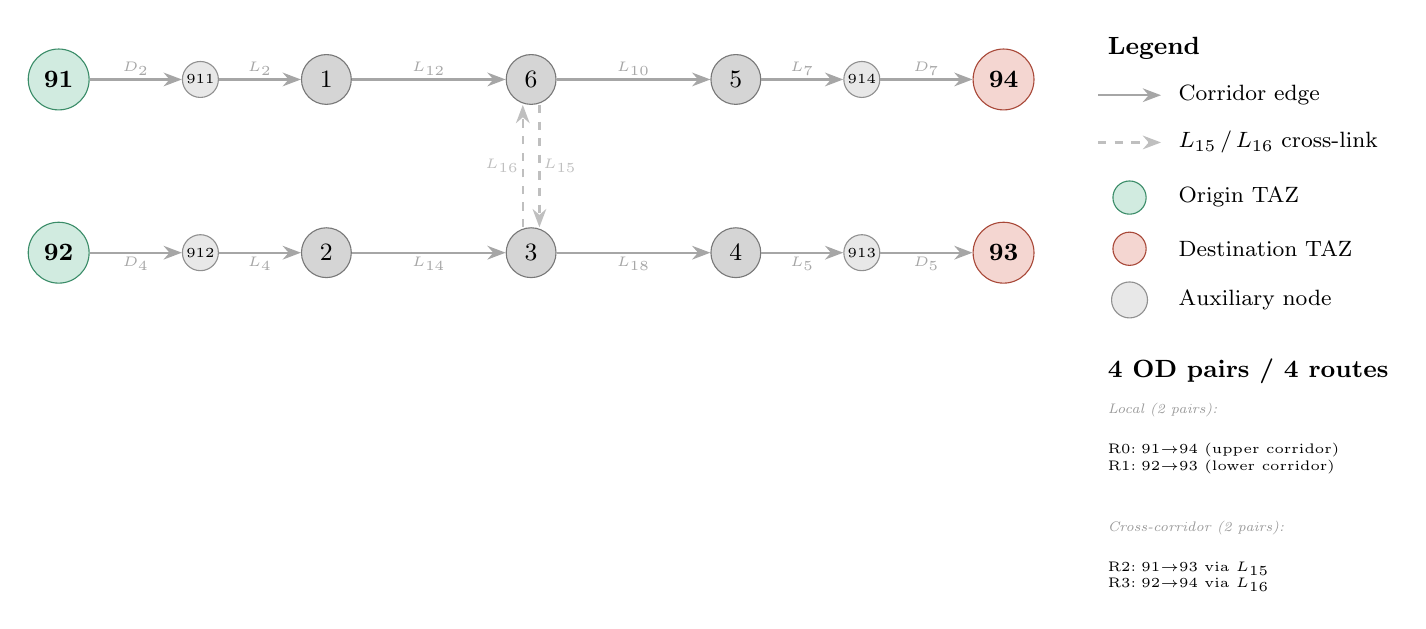
\begin{tikzpicture}[
    >=Stealth,
    onode/.style  = {circle, draw=origincolor!80!black, fill=origincolor!25,
                     minimum size=22pt, inner sep=0pt, font=\small\bfseries},
    dnode/.style  = {circle, draw=destcolor!80!black,   fill=destcolor!25,
                     minimum size=22pt, inner sep=0pt, font=\small\bfseries},
    inode/.style  = {circle, draw=intcolor!80!black,    fill=intcolor!40,
                     minimum size=18pt, inner sep=0pt, font=\small},
    anode/.style  = {circle, draw=auxcolor!80!black,    fill=auxcolor!30,
                     minimum size=13pt, inner sep=0pt, font=\tiny},
    fwd/.style    = {->, thick, gray!70},
    lbl/.style    = {font=\tiny, inner sep=1pt},
]
%% Upper corridor
\node[onode](n91)  at( 0.0,  0.0){91};
\node[anode](a911) at( 1.8,  0.0){\tiny 911};
\node[inode](n1)   at( 3.4,  0.0){1};
\node[inode](n6)   at( 6.0,  0.0){6};
\node[inode](n5)   at( 8.6,  0.0){5};
\node[anode](a914) at(10.2,  0.0){\tiny 914};
\node[dnode](n94)  at(12.0,  0.0){94};
%% Lower corridor
\node[onode](n92)  at( 0.0, -2.2){92};
\node[anode](a912) at( 1.8, -2.2){\tiny 912};
\node[inode](n2)   at( 3.4, -2.2){2};
\node[inode](n3)   at( 6.0, -2.2){3};
\node[inode](n4)   at( 8.6, -2.2){4};
\node[anode](a913) at(10.2, -2.2){\tiny 913};
\node[dnode](n93)  at(12.0, -2.2){93};
%% Upper corridor edges
\draw[fwd](n91)--node[lbl,above]{$D_2$}(a911);
\draw[fwd](a911)--node[lbl,above]{$L_2$}(n1);
\draw[fwd](n1)--node[lbl,above]{$L_{12}$}(n6);
\draw[fwd](n6)--node[lbl,above]{$L_{10}$}(n5);
\draw[fwd](n5)--node[lbl,above]{$L_7$}(a914);
\draw[fwd](a914)--node[lbl,above]{$D_7$}(n94);
%% Lower corridor edges
\draw[fwd](n92)--node[lbl,below]{$D_4$}(a912);
\draw[fwd](a912)--node[lbl,below]{$L_4$}(n2);
\draw[fwd](n2)--node[lbl,below]{$L_{14}$}(n3);
\draw[fwd](n3)--node[lbl,below]{$L_{18}$}(n4);
\draw[fwd](n4)--node[lbl,below]{$L_5$}(a913);
\draw[fwd](a913)--node[lbl,below]{$D_5$}(n93);
%% Cross links
\draw[->,thick,gray!50,dashed]([xshift= 3pt]n6.south)--
    node[lbl,right]{$L_{15}$}([xshift= 3pt]n3.north);
\draw[->,thick,gray!50,dashed]([xshift=-3pt]n3.north)--
    node[lbl,left]{$L_{16}$}([xshift=-3pt]n6.south);
%% Legend + OD table
\begin{scope}[shift={(13.2, 0.4)}]
    \node[font=\small\bfseries,anchor=west]at(0,0){Legend};
    \draw[fwd](0,-0.6)--(0.8,-0.6);
    \node[font=\footnotesize,anchor=west]at(0.9,-0.6){Corridor edge};
    \draw[->,thick,gray!50,dashed](0,-1.2)--(0.8,-1.2);
    \node[font=\footnotesize,anchor=west]at(0.9,-1.2){$L_{15}$\,/\,$L_{16}$ cross-link};
    \node[onode,minimum size=12pt]at(0.4,-1.9){};
    \node[font=\footnotesize,anchor=west]at(0.9,-1.9){Origin TAZ};
    \node[dnode,minimum size=12pt]at(0.4,-2.55){};
    \node[font=\footnotesize,anchor=west]at(0.9,-2.55){Destination TAZ};
    \node[anode]at(0.4,-3.2){};
    \node[font=\footnotesize,anchor=west]at(0.9,-3.2){Auxiliary node};
    \node[font=\small\bfseries,anchor=west]at(0,-4.1){4 OD pairs / 4 routes};
    \node[font=\tiny,text=gray!80,anchor=west]at(0,-4.6){\textit{Local (2 pairs):}};
    \node[font=\tiny,anchor=north west,align=left]at(0,-4.9){%
        R0:\;$91{\to}94$ (upper corridor)\\
        R1:\;$92{\to}93$ (lower corridor)};
    \node[font=\tiny,text=gray!80,anchor=west]at(0,-6.1){\textit{Cross-corridor (2 pairs):}};
    \node[font=\tiny,anchor=north west,align=left]at(0,-6.4){%
        R2:\;$91{\to}93$ via $L_{15}$\\
        R3:\;$92{\to}94$ via $L_{16}$};
\end{scope}
\end{tikzpicture}%
}
\caption{Toy network with all raw SUMO edge IDs. Auxiliary nodes 911--914 are
single-degree merge points that carry identical flow to their adjacent edge and are
therefore absorbed into grouped flow variables (see Figure~\ref{fig:network_toy}).}
\label{fig:network-toy-detail}
\end{figure}

\begin{figure}[h]
\centering
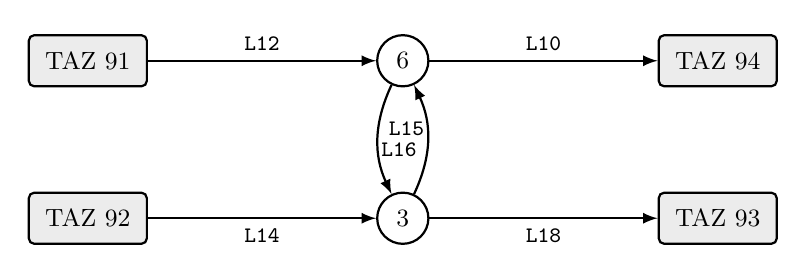
\begin{tikzpicture}[
    taz/.style   = {rectangle, draw, fill=gray!15, rounded corners=2pt,
                    minimum width=1.5cm, minimum height=0.65cm,
                    font=\small},
    junc/.style  = {circle, draw, fill=white, minimum size=0.65cm, font=\small},
    grp/.style   = {font=\footnotesize, midway},
    >=latex, thick
]
  %% Only junctions 6 and 3 survive grouping; 1,2,4,5,911-914 are absorbed.
  \node[taz]  (t91) at (0,2)   {TAZ 91};
  \node[junc] (j6)  at (4,2)   {6};
  \node[taz]  (t94) at (8,2)   {TAZ 94};

  \node[taz]  (t92) at (0,0)   {TAZ 92};
  \node[junc] (j3)  at (4,0)   {3};
  \node[taz]  (t93) at (8,0)   {TAZ 93};

  \draw[->] (t91) -- node[grp, above]{\texttt{L12}} (j6);
  \draw[->] (j6)  -- node[grp, above]{\texttt{L10}} (t94);
  \draw[->] (t92) -- node[grp, below]{\texttt{L14}} (j3);
  \draw[->] (j3)  -- node[grp, below]{\texttt{L18}} (t93);

  \draw[->, bend right=25] (j6) to
      node[right, font=\footnotesize, pos=0.4]{\texttt{L15}} (j3);
  \draw[->, bend right=25] (j3) to
      node[left,  font=\footnotesize, pos=0.4]{\texttt{L16}} (j6);
\end{tikzpicture}
\caption{Toy network after edge grouping. Each group collapses a chain of raw edges
into a single flow variable: \texttt{L12} = \{D2, L2, L12\}, \texttt{L10} = \{D7, L7, L10\},
\texttt{L14} = \{D4, L4, L14\}, \texttt{L18} = \{D5, L5, L18\}.
Intermediate junctions (1, 2, 4, 5) and auxiliary nodes (911--914) are absorbed
and no longer appear.}
\label{fig:network_toy}
\end{figure}

\subsubsection*{Edge-flow groups}

The 6 grouped flow variables used as calibration outputs are listed in
Table~\ref{tab:groups_toy}.

\begin{table}[h]
\centering
\caption{Edge-flow groups for the toy (two-corridor) network.}
\label{tab:groups_toy}
\begin{tabular}{lll}
\hline
\textbf{Group name} & \textbf{Raw SUMO edges} & \textbf{Semantic} \\
\hline
\texttt{L12}  & D2, L2, L12         & TAZ 91 $\to$ junction 6 (entry, upper) \\
\texttt{L14}  & D4, L4, L14         & TAZ 92 $\to$ junction 3 (entry, lower) \\
\texttt{L18}  & D5, L5, L18         & junction 3 $\to$ junction 4 $\to$ TAZ 93 \\
\texttt{L10}  & D7, L7, L10         & junction 6 $\to$ junction 5 $\to$ TAZ 94 \\
\texttt{L15}  & L15                 & junction 6 $\to$ junction 3 (cross-link) \\
\texttt{L16}  & L16                 & junction 3 $\to$ junction 6 (cross-link) \\
\hline
\end{tabular}
\end{table}







%%%%%%%%%%%%%%%%%%%%%%%%%%%%%%%%%%
%%%%%%%%%%%%%%%%%%%%%%%%%%
\subsection{Scaled Network (\texttt{quickstart\_grid\_3})}
\label{app:network_grid3}

\begin{figure}[ht]
\centering
\resizebox{\textwidth}{!}{%
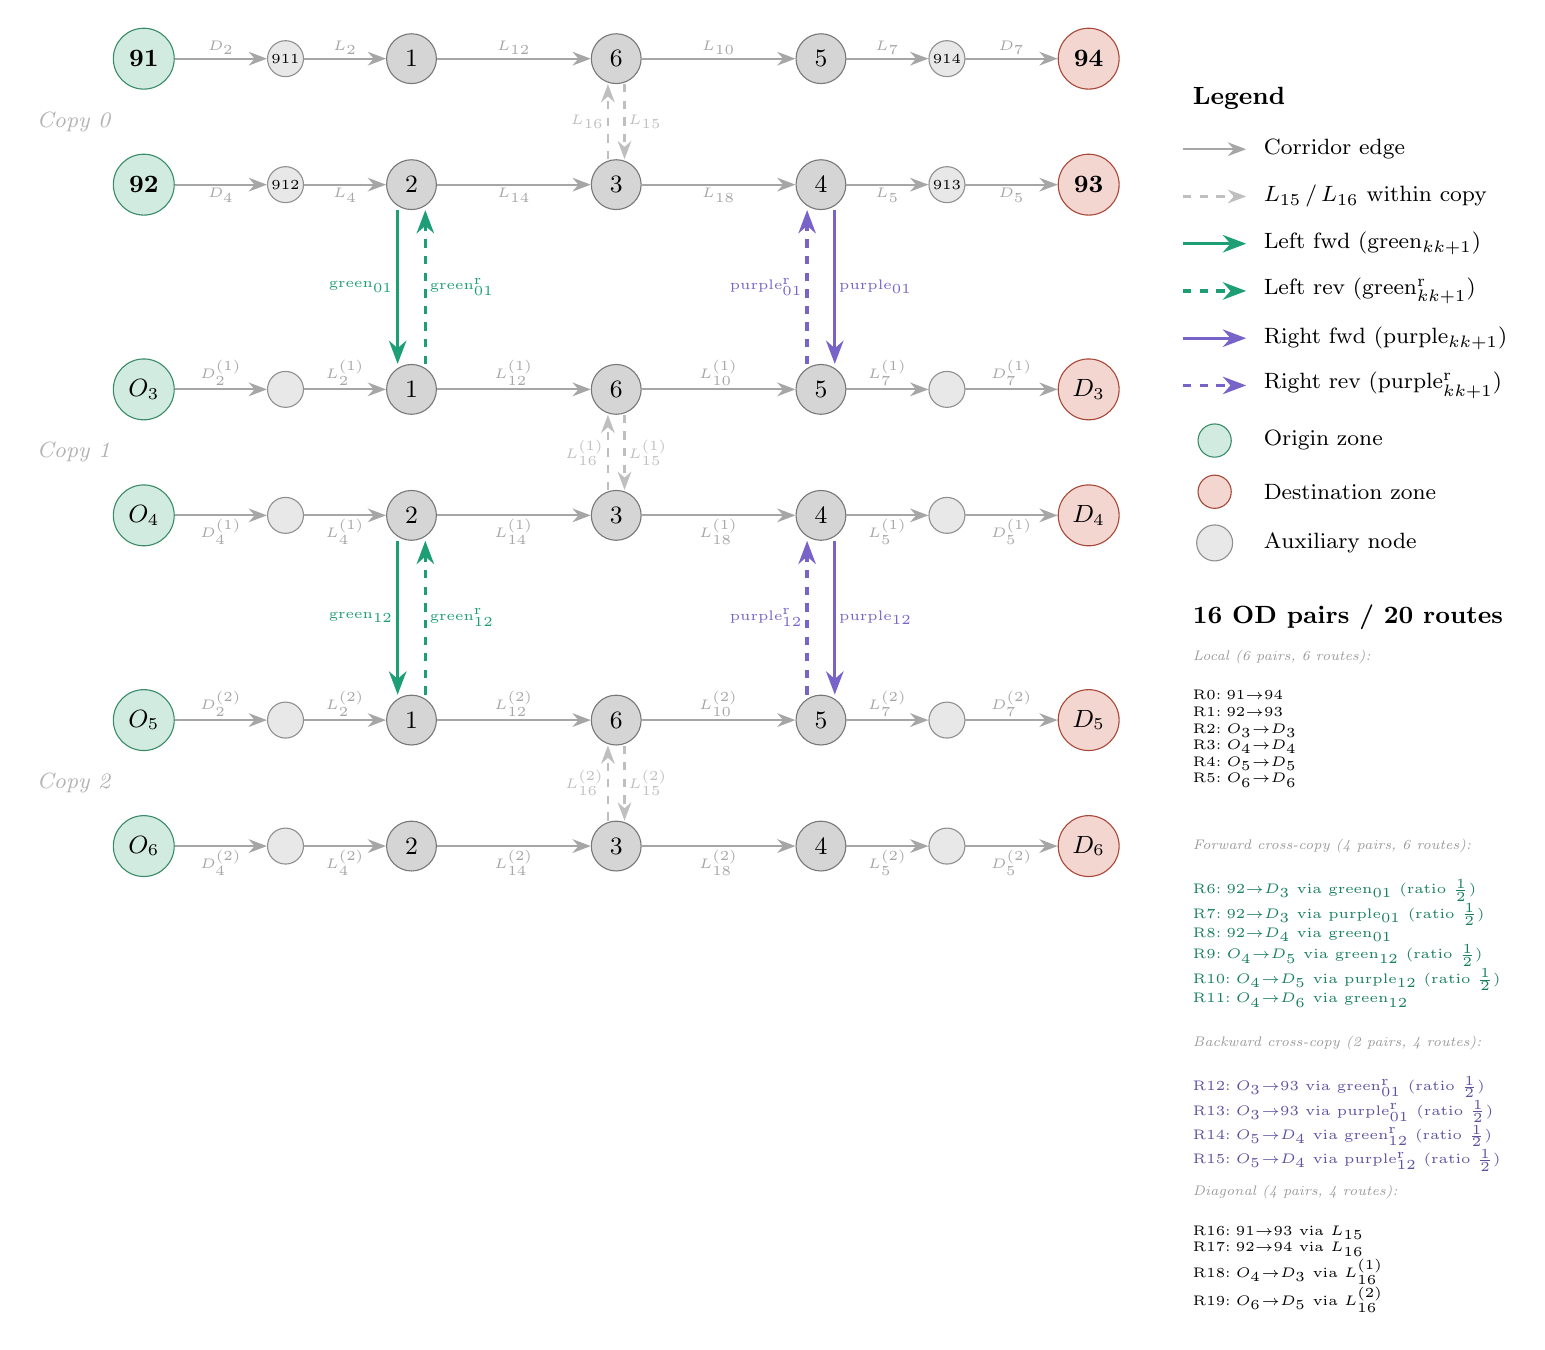
\begin{tikzpicture}[
    >=Stealth,
    onode/.style  = {circle, draw=origincolor!80!black, fill=origincolor!25,
                     minimum size=22pt, inner sep=0pt, font=\small\bfseries},
    dnode/.style  = {circle, draw=destcolor!80!black,   fill=destcolor!25,
                     minimum size=22pt, inner sep=0pt, font=\small\bfseries},
    inode/.style  = {circle, draw=intcolor!80!black,    fill=intcolor!40,
                     minimum size=18pt, inner sep=0pt, font=\small},
    anode/.style  = {circle, draw=auxcolor!80!black,    fill=auxcolor!30,
                     minimum size=13pt, inner sep=0pt, font=\tiny},
    fwd/.style    = {->, thick, gray!70},
    lbl/.style    = {font=\tiny, inner sep=1pt},
    gfwd/.style   = {->, very thick, crossgreen},
    pfwd/.style   = {->, very thick, crosspurple},
    grev/.style   = {->, very thick, crossgreen,  dashed},
    prev/.style   = {->, very thick, crosspurple, dashed},
]

%% ===== NODES =====

%% Copy 0
\node[onode](91)  at( 0.0,  0.0){91};  \node[anode](a91) at( 1.8,  0.0){\tiny 911};
\node[inode](1c0) at( 3.4,  0.0){1};   \node[inode](6c0) at( 6.0,  0.0){6};
\node[inode](5c0) at( 8.6,  0.0){5};   \node[anode](a94) at(10.2,  0.0){\tiny 914};
\node[dnode](94)  at(12.0,  0.0){94};

\node[onode](92)  at( 0.0, -1.6){92};  \node[anode](a92) at( 1.8, -1.6){\tiny 912};
\node[inode](2c0) at( 3.4, -1.6){2};   \node[inode](3c0) at( 6.0, -1.6){3};
\node[inode](4c0) at( 8.6, -1.6){4};   \node[anode](a93) at(10.2, -1.6){\tiny 913};
\node[dnode](93)  at(12.0, -1.6){93};

%% Copy 1
\node[onode](O3)  at( 0.0, -4.2){$O_3$}; \node[anode](a1t1) at( 1.8, -4.2){};
\node[inode](1c1) at( 3.4, -4.2){1};      \node[inode](6c1)  at( 6.0, -4.2){6};
\node[inode](5c1) at( 8.6, -4.2){5};      \node[anode](a1r1) at(10.2, -4.2){};
\node[dnode](D3)  at(12.0, -4.2){$D_3$};

\node[onode](O4)  at( 0.0, -5.8){$O_4$}; \node[anode](a1b1) at( 1.8, -5.8){};
\node[inode](2c1) at( 3.4, -5.8){2};      \node[inode](3c1)  at( 6.0, -5.8){3};
\node[inode](4c1) at( 8.6, -5.8){4};      \node[anode](a1b2) at(10.2, -5.8){};
\node[dnode](D4)  at(12.0, -5.8){$D_4$};

%% Copy 2
\node[onode](O5)  at( 0.0, -8.4){$O_5$}; \node[anode](a2t1) at( 1.8, -8.4){};
\node[inode](1c2) at( 3.4, -8.4){1};      \node[inode](6c2)  at( 6.0, -8.4){6};
\node[inode](5c2) at( 8.6, -8.4){5};      \node[anode](a2r1) at(10.2, -8.4){};
\node[dnode](D5)  at(12.0, -8.4){$D_5$};

\node[onode](O6)  at( 0.0,-10.0){$O_6$}; \node[anode](a2b1) at( 1.8,-10.0){};
\node[inode](2c2) at( 3.4,-10.0){2};      \node[inode](3c2)  at( 6.0,-10.0){3};
\node[inode](4c2) at( 8.6,-10.0){4};      \node[anode](a2b2) at(10.2,-10.0){};
\node[dnode](D6)  at(12.0,-10.0){$D_6$};

%%=============================================================
%%  CORRIDOR EDGES
%%=============================================================

%% Copy 0 — top
\draw[fwd](91) --node[lbl,above]{$D_2$}(a91);
\draw[fwd](a91)--node[lbl,above]{$L_2$}(1c0);
\draw[fwd](1c0)--node[lbl,above]{$L_{12}$}(6c0);
\draw[fwd](6c0)--node[lbl,above]{$L_{10}$}(5c0);
\draw[fwd](5c0)--node[lbl,above]{$L_7$}(a94);
\draw[fwd](a94)--node[lbl,above]{$D_7$}(94);
%% Copy 0 — bottom
\draw[fwd](92) --node[lbl,below]{$D_4$}(a92);
\draw[fwd](a92)--node[lbl,below]{$L_4$}(2c0);
\draw[fwd](2c0)--node[lbl,below]{$L_{14}$}(3c0);
\draw[fwd](3c0)--node[lbl,below]{$L_{18}$}(4c0);
\draw[fwd](4c0)--node[lbl,below]{$L_5$}(a93);
\draw[fwd](a93)--node[lbl,below]{$D_5$}(93);
%% Copy 0 — L15/L16
\draw[->,thick,gray!50,dashed]([xshift= 3pt]6c0.south)--
    node[lbl,right]{$L_{15}$}([xshift= 3pt]3c0.north);
\draw[->,thick,gray!50,dashed]([xshift=-3pt]3c0.north)--
    node[lbl,left]{$L_{16}$}([xshift=-3pt]6c0.south);

%% Copy 1 — top
\draw[fwd](O3) --node[lbl,above]{$D_2^{(1)}$}(a1t1);
\draw[fwd](a1t1)--node[lbl,above]{$L_2^{(1)}$}(1c1);
\draw[fwd](1c1)--node[lbl,above]{$L_{12}^{(1)}$}(6c1);
\draw[fwd](6c1)--node[lbl,above]{$L_{10}^{(1)}$}(5c1);
\draw[fwd](5c1)--node[lbl,above]{$L_7^{(1)}$}(a1r1);
\draw[fwd](a1r1)--node[lbl,above]{$D_7^{(1)}$}(D3);
%% Copy 1 — bottom
\draw[fwd](O4) --node[lbl,below]{$D_4^{(1)}$}(a1b1);
\draw[fwd](a1b1)--node[lbl,below]{$L_4^{(1)}$}(2c1);
\draw[fwd](2c1)--node[lbl,below]{$L_{14}^{(1)}$}(3c1);
\draw[fwd](3c1)--node[lbl,below]{$L_{18}^{(1)}$}(4c1);
\draw[fwd](4c1)--node[lbl,below]{$L_5^{(1)}$}(a1b2);
\draw[fwd](a1b2)--node[lbl,below]{$D_5^{(1)}$}(D4);
%% Copy 1 — L15/L16
\draw[->,thick,gray!50,dashed]([xshift= 3pt]6c1.south)--
    node[lbl,right]{$L_{15}^{(1)}$}([xshift= 3pt]3c1.north);
\draw[->,thick,gray!50,dashed]([xshift=-3pt]3c1.north)--
    node[lbl,left]{$L_{16}^{(1)}$}([xshift=-3pt]6c1.south);

%% Copy 2 — top
\draw[fwd](O5) --node[lbl,above]{$D_2^{(2)}$}(a2t1);
\draw[fwd](a2t1)--node[lbl,above]{$L_2^{(2)}$}(1c2);
\draw[fwd](1c2)--node[lbl,above]{$L_{12}^{(2)}$}(6c2);
\draw[fwd](6c2)--node[lbl,above]{$L_{10}^{(2)}$}(5c2);
\draw[fwd](5c2)--node[lbl,above]{$L_7^{(2)}$}(a2r1);
\draw[fwd](a2r1)--node[lbl,above]{$D_7^{(2)}$}(D5);
%% Copy 2 — bottom
\draw[fwd](O6) --node[lbl,below]{$D_4^{(2)}$}(a2b1);
\draw[fwd](a2b1)--node[lbl,below]{$L_4^{(2)}$}(2c2);
\draw[fwd](2c2)--node[lbl,below]{$L_{14}^{(2)}$}(3c2);
\draw[fwd](3c2)--node[lbl,below]{$L_{18}^{(2)}$}(4c2);
\draw[fwd](4c2)--node[lbl,below]{$L_5^{(2)}$}(a2b2);
\draw[fwd](a2b2)--node[lbl,below]{$D_5^{(2)}$}(D6);
%% Copy 2 — L15/L16
\draw[->,thick,gray!50,dashed]([xshift= 3pt]6c2.south)--
    node[lbl,right]{$L_{15}^{(2)}$}([xshift= 3pt]3c2.north);
\draw[->,thick,gray!50,dashed]([xshift=-3pt]3c2.north)--
    node[lbl,left]{$L_{16}^{(2)}$}([xshift=-3pt]6c2.south);

%%=============================================================
%%  INTER-COPY LINKS
%%=============================================================

\draw[gfwd]([xshift=-5pt]2c0.south)--
    node[lbl,left,text=crossgreen]{$\mathrm{green}_{01}$}
    ([xshift=-5pt]1c1.north);
\draw[grev]([xshift=5pt]1c1.north)--
    node[lbl,right,text=crossgreen]{$\mathrm{green}_{01}^{\mathrm{r}}$}
    ([xshift=5pt]2c0.south);

\draw[gfwd]([xshift=-5pt]2c1.south)--
    node[lbl,left,text=crossgreen]{$\mathrm{green}_{12}$}
    ([xshift=-5pt]1c2.north);
\draw[grev]([xshift=5pt]1c2.north)--
    node[lbl,right,text=crossgreen]{$\mathrm{green}_{12}^{\mathrm{r}}$}
    ([xshift=5pt]2c1.south);

\draw[pfwd]([xshift=5pt]4c0.south)--
    node[lbl,right,text=crosspurple]{$\mathrm{purple}_{01}$}
    ([xshift=5pt]5c1.north);
\draw[prev]([xshift=-5pt]5c1.north)--
    node[lbl,left,text=crosspurple]{$\mathrm{purple}_{01}^{\mathrm{r}}$}
    ([xshift=-5pt]4c0.south);

\draw[pfwd]([xshift=5pt]4c1.south)--
    node[lbl,right,text=crosspurple]{$\mathrm{purple}_{12}$}
    ([xshift=5pt]5c2.north);
\draw[prev]([xshift=-5pt]5c2.north)--
    node[lbl,left,text=crosspurple]{$\mathrm{purple}_{12}^{\mathrm{r}}$}
    ([xshift=-5pt]4c1.south);

%%=============================================================
%%  COPY LABELS
%%=============================================================
\node[font=\footnotesize\itshape,text=gray!60,anchor=east]
    at(-0.3,-0.8){Copy 0};
\node[font=\footnotesize\itshape,text=gray!60,anchor=east]
    at(-0.3,-5.0){Copy 1};
\node[font=\footnotesize\itshape,text=gray!60,anchor=east]
    at(-0.3,-9.2){Copy 2};

%%=============================================================
%%  LEGEND + OD TABLE
%%=============================================================
\begin{scope}[shift={(13.2,-0.5)}]

    \node[font=\small\bfseries,anchor=west]at(0,0){Legend};

    \draw[fwd](0,-0.65)--(0.8,-0.65);
    \node[font=\footnotesize,anchor=west]at(0.9,-0.65){Corridor edge};

    \draw[->,thick,gray!50,dashed](0,-1.25)--(0.8,-1.25);
    \node[font=\footnotesize,anchor=west]at(0.9,-1.25){%
        $L_{15}$\,/\,$L_{16}$ within copy};

    \draw[gfwd](0,-1.85)--(0.8,-1.85);
    \node[font=\footnotesize,anchor=west]at(0.9,-1.85){%
        Left fwd (green$_{kk+1}$)};

    \draw[grev](0,-2.45)--(0.8,-2.45);
    \node[font=\footnotesize,anchor=west]at(0.9,-2.45){%
        Left rev (green$^{\mathrm{r}}_{kk+1}$)};

    \draw[pfwd](0,-3.05)--(0.8,-3.05);
    \node[font=\footnotesize,anchor=west]at(0.9,-3.05){%
        Right fwd (purple$_{kk+1}$)};

    \draw[prev](0,-3.65)--(0.8,-3.65);
    \node[font=\footnotesize,anchor=west]at(0.9,-3.65){%
        Right rev (purple$^{\mathrm{r}}_{kk+1}$)};

    \node[onode,minimum size=12pt]at(0.4,-4.35){};
    \node[font=\footnotesize,anchor=west]at(0.9,-4.35){Origin zone};

    \node[dnode,minimum size=12pt]at(0.4,-5.0){};
    \node[font=\footnotesize,anchor=west]at(0.9,-5.0){Destination zone};

    \node[anode]at(0.4,-5.65){};
    \node[font=\footnotesize,anchor=west]at(0.9,-5.65){Auxiliary node};

    %% OD table
    \node[font=\small\bfseries,anchor=west]at(0,-6.6){%
        16 OD pairs / 20 routes};

    \node[font=\tiny,text=gray!80,anchor=west]at(0,-7.1){%
        \textit{Local (6 pairs, 6 routes):}};
    \node[font=\tiny,anchor=north west,align=left]at(0,-7.4){%
        R0:\;$91{\to}94$\\
        R1:\;$92{\to}93$\\
        R2:\;$O_3{\to}D_3$\\
        R3:\;$O_4{\to}D_4$\\
        R4:\;$O_5{\to}D_5$\\
        R5:\;$O_6{\to}D_6$};

    \node[font=\tiny,text=gray!80,anchor=west]at(0,-9.5){%
        \textit{Forward cross-copy (4 pairs, 6 routes):}};
    \node[font=\tiny,anchor=north west,align=left,
          text=crossgreen!80!black]at(0,-9.8){%
        R6:\;$92{\to}D_3$ via green$_{01}$ (ratio $\tfrac{1}{2}$)\\
        R7:\;$92{\to}D_3$ via purple$_{01}$ (ratio $\tfrac{1}{2}$)\\
        R8:\;$92{\to}D_4$ via green$_{01}$\\
        R9:\;$O_4{\to}D_5$ via green$_{12}$ (ratio $\tfrac{1}{2}$)\\
        R10:\;$O_4{\to}D_5$ via purple$_{12}$ (ratio $\tfrac{1}{2}$)\\
        R11:\;$O_4{\to}D_6$ via green$_{12}$};

    \node[font=\tiny,text=gray!80,anchor=west]at(0,-12.0){%
        \textit{Backward cross-copy (2 pairs, 4 routes):}};
    \node[font=\tiny,anchor=north west,align=left,
          text=crosspurple!80!black]at(0,-12.3){%
        R12:\;$O_3{\to}93$ via green$_{01}^{\mathrm{r}}$
              (ratio $\tfrac{1}{2}$)\\
        R13:\;$O_3{\to}93$ via purple$_{01}^{\mathrm{r}}$
              (ratio $\tfrac{1}{2}$)\\
        R14:\;$O_5{\to}D_4$ via green$_{12}^{\mathrm{r}}$
              (ratio $\tfrac{1}{2}$)\\
        R15:\;$O_5{\to}D_4$ via purple$_{12}^{\mathrm{r}}$
              (ratio $\tfrac{1}{2}$)};

    \node[font=\tiny,text=gray!80,anchor=west]at(0,-13.9){%
        \textit{Diagonal (4 pairs, 4 routes):}};
    \node[font=\tiny,anchor=north west,align=left]at(0,-14.2){%
        R16:\;$91{\to}93$ via $L_{15}$\\
        R17:\;$92{\to}94$ via $L_{16}$\\
        R18:\;$O_4{\to}D_3$ via $L_{16}^{(1)}$\\
        R19:\;$O_6{\to}D_5$ via $L_{16}^{(2)}$};

\end{scope}

\end{tikzpicture}%
}
\caption{Three-corridor synthetic network (\texttt{quickstart\_grid\_3}).
Green and purple arrows denote cross-corridor connectors;
dashed arrows within each corridor are the $L_{15}$\,/\,$L_{16}$
diagonal links.}
\label{fig:network-grid3}
\end{figure}


\subsubsection*{Topology}

The \texttt{quickstart\_grid\_3} network is constructed by replicating the
two-corridor base module three times (copies 0, 1, 2) and connecting adjacent
copies at their left and right interior junctions via bidirectional
\emph{green} and \emph{purple} cross-streets
(Figure~\ref{fig:network-grid3}).
This yields 6 origin TAZs, 6 destination TAZs, and 36 grouped flow variables.

\subsubsection*{Grouping methodology}

Within each copy, the same forced-chain logic as the toy network applies:
connector \texttt{D}-edges and short intermediate \texttt{L}-edges adjacent to
a TAZ always carry identical flow and are merged into the nearest
corridor-level edge ID.
In copy~2 specifically, junctions $2_2$ and $4_2$ have no downstream copy
to receive green/purple traffic, so their \texttt{L14} and \texttt{L18}
segments are also pass-through and are absorbed into the \texttt{c2\_in\_O6}
and \texttt{c2\_out\_D6} groups respectively.
Cross-copy edges (\texttt{green\_*}, \texttt{purple\_*}) are single-edge
links with no merges and therefore each form their own singleton group.

\subsubsection*{Edge-flow groups}

The full list of 36 grouped flow variables is given in
Tables~\ref{tab:groups_grid3_c0}--\ref{tab:groups_grid3_c2}.

% ,- Copy 0 ,-
\begin{table}[h]
\centering
\caption{Edge-flow groups: copy~0 and cross-copy 0$\leftrightarrow$1.}
\label{tab:groups_grid3_c0}
\begin{tabular}{lll}
\hline
\textbf{Group name} & \textbf{Raw SUMO edges} & \textbf{Semantic} \\
\hline
\multicolumn{3}{l}{\textit{Copy 0 (origins 91, 92; destinations 94, 93)}} \\
\texttt{c0\_in\_91}  & c0\_D2, c0\_L2, c0\_L12  & TAZ 91 $\to$ junction $6_0$ \\
\texttt{c0\_out\_94} & c0\_L10, c0\_L7, c0\_D7  & junction $6_0$ $\to$ TAZ 94 \\
\texttt{c0\_L15}     & c0\_L15                  & $6_0 \to 3_0$ (cross-link) \\
\texttt{c0\_L16}     & c0\_L16                  & $3_0 \to 6_0$ (cross-link) \\
\texttt{c0\_in\_92}  & c0\_D4, c0\_L4           & TAZ 92 $\to$ junction $2_0$ \\
\texttt{c0\_L14}     & c0\_L14                  & $2_0 \to 3_0$ \\
\texttt{c0\_L18}     & c0\_L18                  & $3_0 \to 4_0$ \\
\texttt{c0\_out\_93} & c0\_L5, c0\_D5           & junction $4_0$ $\to$ TAZ 93 \\
\hline
\multicolumn{3}{l}{\textit{Cross-copy 0 $\leftrightarrow$ 1}} \\
\texttt{green\_01}   & green\_01                & $2_0 \to 1_1$ \\
\texttt{green\_01\_r}& green\_01\_r             & $1_1 \to 2_0$ \\
\texttt{purple\_01}  & purple\_01               & $4_0 \to 5_1$ \\
\texttt{purple\_01\_r}& purple\_01\_r           & $5_1 \to 4_0$ \\
\hline
\end{tabular}
\end{table}

% ,- Copy 1 ,-
\begin{table}[h]
\centering
\caption{Edge-flow groups: copy~1 and cross-copy 1$\leftrightarrow$2.}
\label{tab:groups_grid3_c1}
\begin{tabular}{lll}
\hline
\textbf{Group name} & \textbf{Raw SUMO edges} & \textbf{Semantic} \\
\hline
\multicolumn{3}{l}{\textit{Copy 1 (origins O3, O4; destinations D3, D4)}} \\
\texttt{c1\_in\_O3}  & c1\_D2, c1\_L2           & TAZ O3 $\to$ junction $1_1$ \\
\texttt{c1\_L12}     & c1\_L12                  & $1_1 \to 6_1$ \\
\texttt{c1\_L10}     & c1\_L10                  & $6_1 \to 5_1$ \\
\texttt{c1\_L15}     & c1\_L15                  & $6_1 \to 3_1$ (cross-link) \\
\texttt{c1\_L16}     & c1\_L16                  & $3_1 \to 6_1$ (cross-link) \\
\texttt{c1\_out\_D3} & c1\_L7, c1\_D7           & junction $5_1$ $\to$ TAZ D3 \\
\texttt{c1\_in\_O4}  & c1\_D4, c1\_L4           & TAZ O4 $\to$ junction $2_1$ \\
\texttt{c1\_L14}     & c1\_L14                  & $2_1 \to 3_1$ \\
\texttt{c1\_L18}     & c1\_L18                  & $3_1 \to 4_1$ \\
\texttt{c1\_out\_D4} & c1\_L5, c1\_D5           & junction $4_1$ $\to$ TAZ D4 \\
\hline
\multicolumn{3}{l}{\textit{Cross-copy 1 $\leftrightarrow$ 2}} \\
\texttt{green\_12}   & green\_12                & $2_1 \to 1_2$ \\
\texttt{green\_12\_r}& green\_12\_r             & $1_2 \to 2_1$ \\
\texttt{purple\_12}  & purple\_12               & $4_1 \to 5_2$ \\
\texttt{purple\_12\_r}& purple\_12\_r           & $5_2 \to 4_1$ \\
\hline
\end{tabular}
\end{table}

% ,- Copy 2 ,-
\begin{table}[h]
\centering
\caption{Edge-flow groups: copy~2 (terminal; no downstream copy).}
\label{tab:groups_grid3_c2}
\begin{tabular}{lll}
\hline
\textbf{Group name} & \textbf{Raw SUMO edges} & \textbf{Semantic} \\
\hline
\texttt{c2\_in\_O5}  & c2\_D2, c2\_L2                     & TAZ O5 $\to$ junction $1_2$ \\
\texttt{c2\_L12}     & c2\_L12                            & $1_2 \to 6_2$ \\
\texttt{c2\_L10}     & c2\_L10                            & $6_2 \to 5_2$ \\
\texttt{c2\_L15}     & c2\_L15                            & $6_2 \to 3_2$ (cross-link) \\
\texttt{c2\_L16}     & c2\_L16                            & $3_2 \to 6_2$ (cross-link) \\
\texttt{c2\_out\_D5} & c2\_L7, c2\_D7                     & junction $5_2$ $\to$ TAZ D5 \\
\texttt{c2\_in\_O6}  & c2\_D4, c2\_L4, c2\_L14            & TAZ O6 $\to$ junction $3_2$\rlap{$^*$} \\
\texttt{c2\_out\_D6} & c2\_L18, c2\_L5, c2\_D5            & junction $3_2$ $\to$ TAZ D6\rlap{$^*$} \\
\hline
\multicolumn{3}{l}{\small $^*$ Junction $2_2$ and $4_2$ are pass-through: L14 and L18 are absorbed into}\\
\multicolumn{3}{l}{\small \phantom{$^*$} the entry/exit chains because copy~2 has no downstream copy.}\\
\hline
\end{tabular}
\end{table}



\subsection{Dense Generated Network (\texttt{quickstart\_grid\_3\_dense})}
\label{subsec:dense-network}

\begin{figure}[ht]
\centering
\resizebox{\textwidth}{!}{%
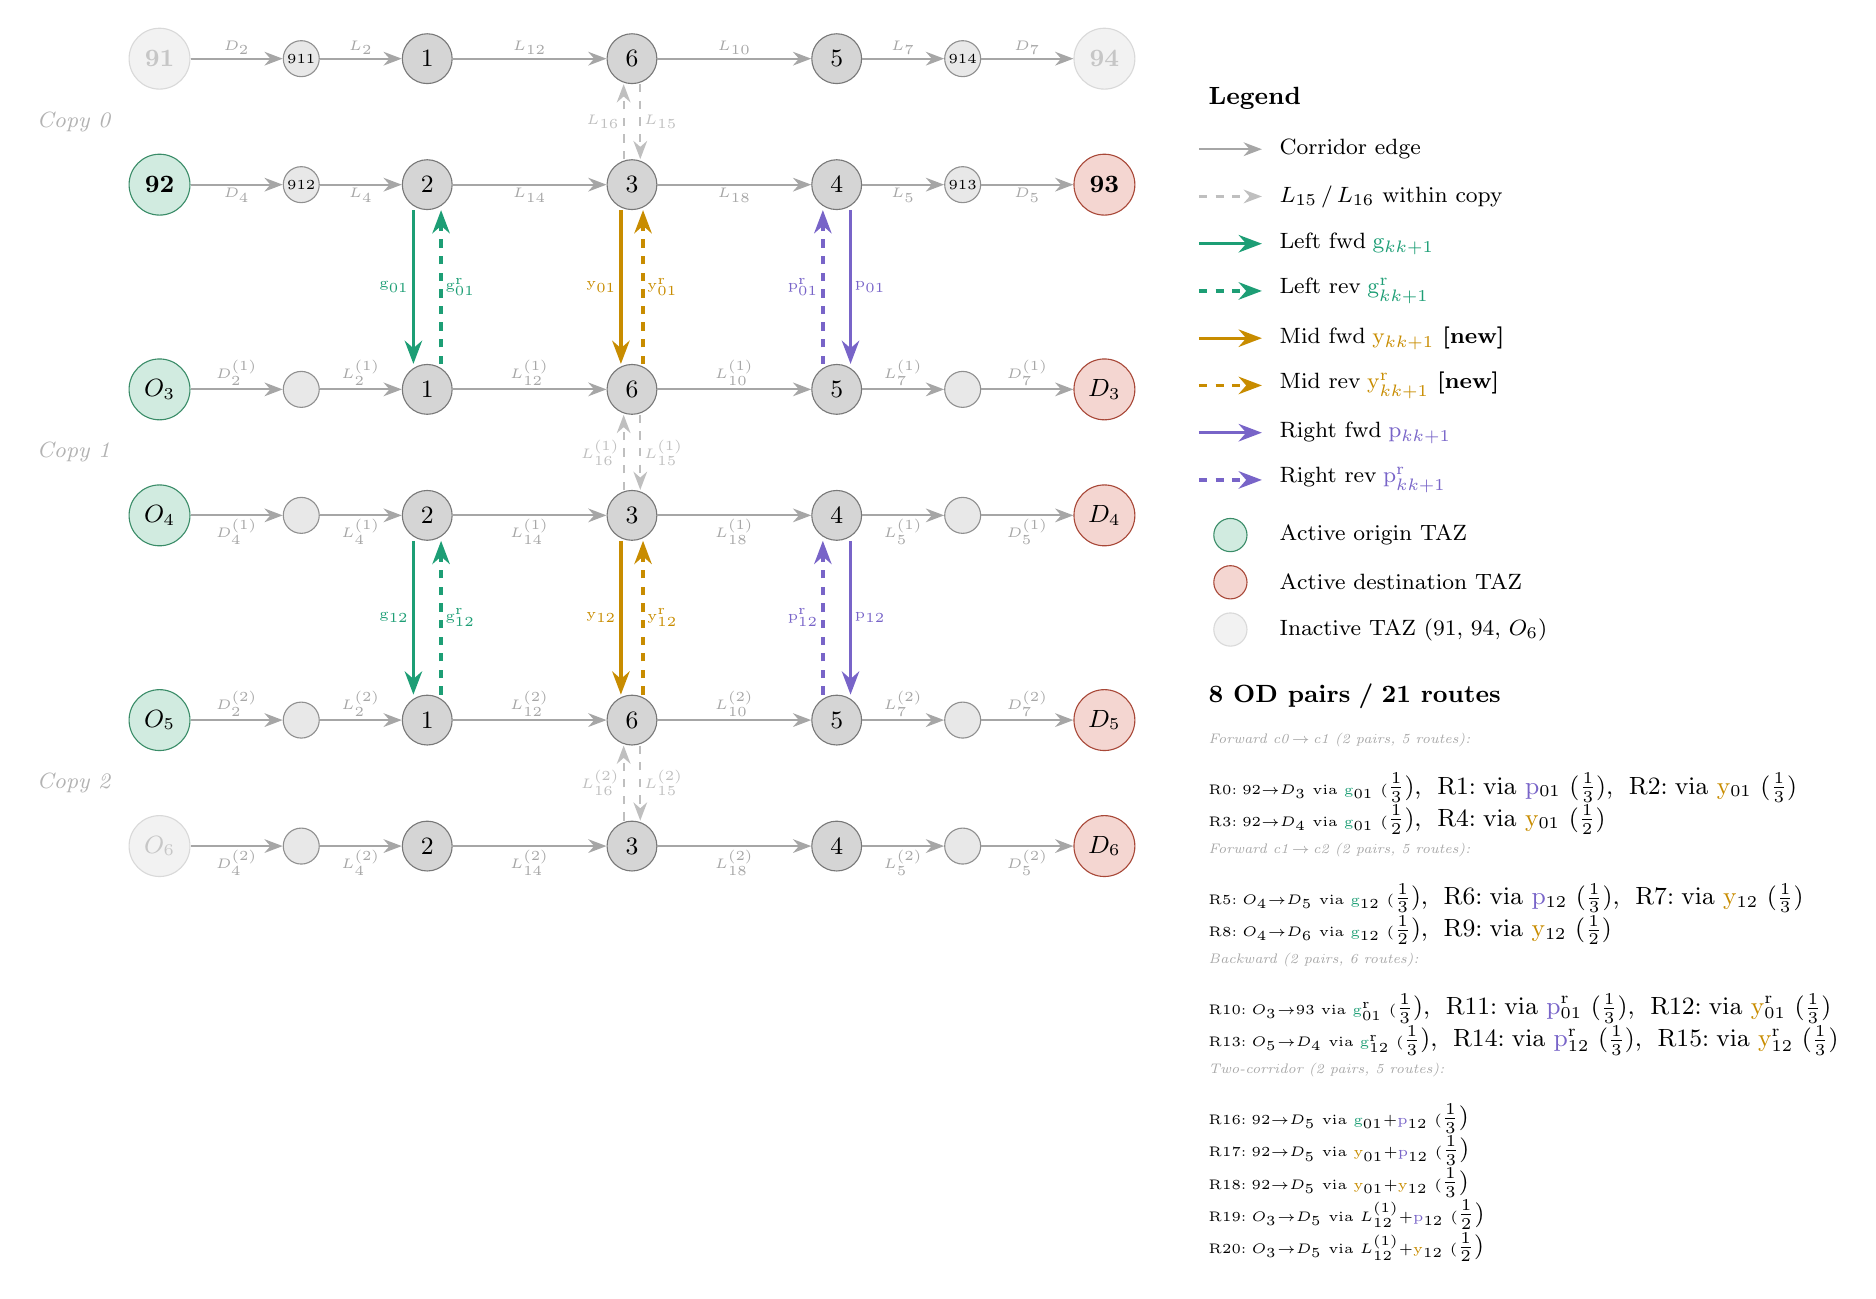
\begin{tikzpicture}[
    >=Stealth,
    onode/.style  = {circle, draw=origincolor!80!black, fill=origincolor!25,
                     minimum size=22pt, inner sep=0pt, font=\small\bfseries},
    dnode/.style  = {circle, draw=destcolor!80!black,   fill=destcolor!25,
                     minimum size=22pt, inner sep=0pt, font=\small\bfseries},
    inode/.style  = {circle, draw=intcolor!80!black,    fill=intcolor!40,
                     minimum size=18pt, inner sep=0pt, font=\small},
    anode/.style  = {circle, draw=auxcolor!80!black,    fill=auxcolor!30,
                     minimum size=13pt, inner sep=0pt, font=\tiny},
    unode/.style  = {circle, draw=gray!30, fill=gray!10,
                     minimum size=22pt, inner sep=0pt,
                     font=\small\bfseries, text=gray!45},
    fwd/.style    = {->, thick, gray!70},
    lbl/.style    = {font=\tiny, inner sep=1pt},
    gfwd/.style   = {->, very thick, crossgreen},
    pfwd/.style   = {->, very thick, crosspurple},
    yfwd/.style   = {->, very thick, crossyellow},
    grev/.style   = {->, very thick, crossgreen,  dashed},
    prev/.style   = {->, very thick, crosspurple, dashed},
    yrev/.style   = {->, very thick, crossyellow, dashed},
]

%% ===== NODES =====

%% Copy 0 — top (91 and 94 inactive in this experiment)
\node[unode](91)  at( 0.0,  0.0){91};  \node[anode](a91) at( 1.8,  0.0){\tiny 911};
\node[inode](1c0) at( 3.4,  0.0){1};   \node[inode](6c0) at( 6.0,  0.0){6};
\node[inode](5c0) at( 8.6,  0.0){5};   \node[anode](a94) at(10.2,  0.0){\tiny 914};
\node[unode](94)  at(12.0,  0.0){94};

%% Copy 0 — bottom (92 active origin, 93 active destination)
\node[onode](92)  at( 0.0, -1.6){92};  \node[anode](a92) at( 1.8, -1.6){\tiny 912};
\node[inode](2c0) at( 3.4, -1.6){2};   \node[inode](3c0) at( 6.0, -1.6){3};
\node[inode](4c0) at( 8.6, -1.6){4};   \node[anode](a93) at(10.2, -1.6){\tiny 913};
\node[dnode](93)  at(12.0, -1.6){93};

%% Copy 1 — top (O3 active origin, D3 active destination)
\node[onode](O3)  at( 0.0, -4.2){$O_3$}; \node[anode](a1t1) at( 1.8, -4.2){};
\node[inode](1c1) at( 3.4, -4.2){1};      \node[inode](6c1)  at( 6.0, -4.2){6};
\node[inode](5c1) at( 8.6, -4.2){5};      \node[anode](a1r1) at(10.2, -4.2){};
\node[dnode](D3)  at(12.0, -4.2){$D_3$};

%% Copy 1 — bottom (O4 active origin, D4 active destination)
\node[onode](O4)  at( 0.0, -5.8){$O_4$}; \node[anode](a1b1) at( 1.8, -5.8){};
\node[inode](2c1) at( 3.4, -5.8){2};      \node[inode](3c1)  at( 6.0, -5.8){3};
\node[inode](4c1) at( 8.6, -5.8){4};      \node[anode](a1b2) at(10.2, -5.8){};
\node[dnode](D4)  at(12.0, -5.8){$D_4$};

%% Copy 2 — top (O5 active origin, D5 active destination)
\node[onode](O5)  at( 0.0, -8.4){$O_5$}; \node[anode](a2t1) at( 1.8, -8.4){};
\node[inode](1c2) at( 3.4, -8.4){1};      \node[inode](6c2)  at( 6.0, -8.4){6};
\node[inode](5c2) at( 8.6, -8.4){5};      \node[anode](a2r1) at(10.2, -8.4){};
\node[dnode](D5)  at(12.0, -8.4){$D_5$};

%% Copy 2 — bottom (O6 inactive, D6 active destination)
\node[unode](O6)  at( 0.0,-10.0){$O_6$}; \node[anode](a2b1) at( 1.8,-10.0){};
\node[inode](2c2) at( 3.4,-10.0){2};      \node[inode](3c2)  at( 6.0,-10.0){3};
\node[inode](4c2) at( 8.6,-10.0){4};      \node[anode](a2b2) at(10.2,-10.0){};
\node[dnode](D6)  at(12.0,-10.0){$D_6$};

%%=============================================================
%%  CORRIDOR EDGES (identical structure to quickstart_grid_3)
%%=============================================================

%% Copy 0 — top
\draw[fwd](91) --node[lbl,above]{$D_2$}(a91);
\draw[fwd](a91)--node[lbl,above]{$L_2$}(1c0);
\draw[fwd](1c0)--node[lbl,above]{$L_{12}$}(6c0);
\draw[fwd](6c0)--node[lbl,above]{$L_{10}$}(5c0);
\draw[fwd](5c0)--node[lbl,above]{$L_7$}(a94);
\draw[fwd](a94)--node[lbl,above]{$D_7$}(94);
%% Copy 0 — bottom
\draw[fwd](92) --node[lbl,below]{$D_4$}(a92);
\draw[fwd](a92)--node[lbl,below]{$L_4$}(2c0);
\draw[fwd](2c0)--node[lbl,below]{$L_{14}$}(3c0);
\draw[fwd](3c0)--node[lbl,below]{$L_{18}$}(4c0);
\draw[fwd](4c0)--node[lbl,below]{$L_5$}(a93);
\draw[fwd](a93)--node[lbl,below]{$D_5$}(93);
%% Copy 0 — L15/L16
\draw[->,thick,gray!50,dashed]([xshift= 3pt]6c0.south)--
    node[lbl,right]{$L_{15}$}([xshift= 3pt]3c0.north);
\draw[->,thick,gray!50,dashed]([xshift=-3pt]3c0.north)--
    node[lbl,left]{$L_{16}$}([xshift=-3pt]6c0.south);

%% Copy 1 — top
\draw[fwd](O3) --node[lbl,above]{$D_2^{(1)}$}(a1t1);
\draw[fwd](a1t1)--node[lbl,above]{$L_2^{(1)}$}(1c1);
\draw[fwd](1c1)--node[lbl,above]{$L_{12}^{(1)}$}(6c1);
\draw[fwd](6c1)--node[lbl,above]{$L_{10}^{(1)}$}(5c1);
\draw[fwd](5c1)--node[lbl,above]{$L_7^{(1)}$}(a1r1);
\draw[fwd](a1r1)--node[lbl,above]{$D_7^{(1)}$}(D3);
%% Copy 1 — bottom
\draw[fwd](O4) --node[lbl,below]{$D_4^{(1)}$}(a1b1);
\draw[fwd](a1b1)--node[lbl,below]{$L_4^{(1)}$}(2c1);
\draw[fwd](2c1)--node[lbl,below]{$L_{14}^{(1)}$}(3c1);
\draw[fwd](3c1)--node[lbl,below]{$L_{18}^{(1)}$}(4c1);
\draw[fwd](4c1)--node[lbl,below]{$L_5^{(1)}$}(a1b2);
\draw[fwd](a1b2)--node[lbl,below]{$D_5^{(1)}$}(D4);
%% Copy 1 — L15/L16
\draw[->,thick,gray!50,dashed]([xshift= 3pt]6c1.south)--
    node[lbl,right]{$L_{15}^{(1)}$}([xshift= 3pt]3c1.north);
\draw[->,thick,gray!50,dashed]([xshift=-3pt]3c1.north)--
    node[lbl,left]{$L_{16}^{(1)}$}([xshift=-3pt]6c1.south);

%% Copy 2 — top
\draw[fwd](O5) --node[lbl,above]{$D_2^{(2)}$}(a2t1);
\draw[fwd](a2t1)--node[lbl,above]{$L_2^{(2)}$}(1c2);
\draw[fwd](1c2)--node[lbl,above]{$L_{12}^{(2)}$}(6c2);
\draw[fwd](6c2)--node[lbl,above]{$L_{10}^{(2)}$}(5c2);
\draw[fwd](5c2)--node[lbl,above]{$L_7^{(2)}$}(a2r1);
\draw[fwd](a2r1)--node[lbl,above]{$D_7^{(2)}$}(D5);
%% Copy 2 — bottom
\draw[fwd](O6) --node[lbl,below]{$D_4^{(2)}$}(a2b1);
\draw[fwd](a2b1)--node[lbl,below]{$L_4^{(2)}$}(2c2);
\draw[fwd](2c2)--node[lbl,below]{$L_{14}^{(2)}$}(3c2);
\draw[fwd](3c2)--node[lbl,below]{$L_{18}^{(2)}$}(4c2);
\draw[fwd](4c2)--node[lbl,below]{$L_5^{(2)}$}(a2b2);
\draw[fwd](a2b2)--node[lbl,below]{$D_5^{(2)}$}(D6);
%% Copy 2 — L15/L16
\draw[->,thick,gray!50,dashed]([xshift= 3pt]6c2.south)--
    node[lbl,right]{$L_{15}^{(2)}$}([xshift= 3pt]3c2.north);
\draw[->,thick,gray!50,dashed]([xshift=-3pt]3c2.north)--
    node[lbl,left]{$L_{16}^{(2)}$}([xshift=-3pt]6c2.south);

%%=============================================================
%%  INTER-COPY LINKS: green (left, x=3.4)
%%=============================================================

\draw[gfwd]([xshift=-5pt]2c0.south)--
    node[lbl,left,text=crossgreen]{$\mathrm{g}_{01}$}
    ([xshift=-5pt]1c1.north);
\draw[grev]([xshift=5pt]1c1.north)--
    node[lbl,right,text=crossgreen]{$\mathrm{g}_{01}^{\mathrm{r}}$}
    ([xshift=5pt]2c0.south);

\draw[gfwd]([xshift=-5pt]2c1.south)--
    node[lbl,left,text=crossgreen]{$\mathrm{g}_{12}$}
    ([xshift=-5pt]1c2.north);
\draw[grev]([xshift=5pt]1c2.north)--
    node[lbl,right,text=crossgreen]{$\mathrm{g}_{12}^{\mathrm{r}}$}
    ([xshift=5pt]2c1.south);

%%=============================================================
%%  INTER-COPY LINKS: yellow (middle, x=6.0) — NEW
%%=============================================================

\draw[yfwd]([xshift=-4pt]3c0.south)--
    node[lbl,left,text=crossyellow]{$\mathrm{y}_{01}$}
    ([xshift=-4pt]6c1.north);
\draw[yrev]([xshift=4pt]6c1.north)--
    node[lbl,right,text=crossyellow]{$\mathrm{y}_{01}^{\mathrm{r}}$}
    ([xshift=4pt]3c0.south);

\draw[yfwd]([xshift=-4pt]3c1.south)--
    node[lbl,left,text=crossyellow]{$\mathrm{y}_{12}$}
    ([xshift=-4pt]6c2.north);
\draw[yrev]([xshift=4pt]6c2.north)--
    node[lbl,right,text=crossyellow]{$\mathrm{y}_{12}^{\mathrm{r}}$}
    ([xshift=4pt]3c1.south);

%%=============================================================
%%  INTER-COPY LINKS: purple (right, x=8.6)
%%=============================================================

\draw[pfwd]([xshift=5pt]4c0.south)--
    node[lbl,right,text=crosspurple]{$\mathrm{p}_{01}$}
    ([xshift=5pt]5c1.north);
\draw[prev]([xshift=-5pt]5c1.north)--
    node[lbl,left,text=crosspurple]{$\mathrm{p}_{01}^{\mathrm{r}}$}
    ([xshift=-5pt]4c0.south);

\draw[pfwd]([xshift=5pt]4c1.south)--
    node[lbl,right,text=crosspurple]{$\mathrm{p}_{12}$}
    ([xshift=5pt]5c2.north);
\draw[prev]([xshift=-5pt]5c2.north)--
    node[lbl,left,text=crosspurple]{$\mathrm{p}_{12}^{\mathrm{r}}$}
    ([xshift=-5pt]4c1.south);

%%=============================================================
%%  COPY LABELS
%%=============================================================
\node[font=\footnotesize\itshape,text=gray!60,anchor=east]
    at(-0.5,-0.8){Copy 0};
\node[font=\footnotesize\itshape,text=gray!60,anchor=east]
    at(-0.5,-5.0){Copy 1};
\node[font=\footnotesize\itshape,text=gray!60,anchor=east]
    at(-0.5,-9.2){Copy 2};

%%=============================================================
%%  LEGEND + OD TABLE (sidebar)
%%=============================================================
\begin{scope}[shift={(13.2,-0.5)}]

    \node[font=\small\bfseries,anchor=west]at(0,0){Legend};

    \draw[fwd](0,-0.65)--(0.8,-0.65);
    \node[font=\footnotesize,anchor=west]at(0.9,-0.65){Corridor edge};

    \draw[->,thick,gray!50,dashed](0,-1.25)--(0.8,-1.25);
    \node[font=\footnotesize,anchor=west]at(0.9,-1.25){%
        $L_{15}$\,/\,$L_{16}$ within copy};

    \draw[gfwd](0,-1.85)--(0.8,-1.85);
    \node[font=\footnotesize,anchor=west]at(0.9,-1.85){%
        Left fwd\;\textcolor{crossgreen}{$\mathrm{g}_{kk{+}1}$}};

    \draw[grev](0,-2.45)--(0.8,-2.45);
    \node[font=\footnotesize,anchor=west]at(0.9,-2.45){%
        Left rev\;\textcolor{crossgreen}{$\mathrm{g}_{kk{+}1}^{\mathrm{r}}$}};

    \draw[yfwd](0,-3.05)--(0.8,-3.05);
    \node[font=\footnotesize,anchor=west]at(0.9,-3.05){%
        Mid fwd\;\textcolor{crossyellow}{$\mathrm{y}_{kk{+}1}$} \textbf{[new]}};

    \draw[yrev](0,-3.65)--(0.8,-3.65);
    \node[font=\footnotesize,anchor=west]at(0.9,-3.65){%
        Mid rev\;\textcolor{crossyellow}{$\mathrm{y}_{kk{+}1}^{\mathrm{r}}$} \textbf{[new]}};

    \draw[pfwd](0,-4.25)--(0.8,-4.25);
    \node[font=\footnotesize,anchor=west]at(0.9,-4.25){%
        Right fwd\;\textcolor{crosspurple}{$\mathrm{p}_{kk{+}1}$}};

    \draw[prev](0,-4.85)--(0.8,-4.85);
    \node[font=\footnotesize,anchor=west]at(0.9,-4.85){%
        Right rev\;\textcolor{crosspurple}{$\mathrm{p}_{kk{+}1}^{\mathrm{r}}$}};

    \node[onode,minimum size=12pt]at(0.4,-5.55){};
    \node[font=\footnotesize,anchor=west]at(0.9,-5.55){Active origin TAZ};

    \node[dnode,minimum size=12pt]at(0.4,-6.15){};
    \node[font=\footnotesize,anchor=west]at(0.9,-6.15){Active destination TAZ};

    \node[unode,minimum size=12pt]at(0.4,-6.75){};
    \node[font=\footnotesize,anchor=west]at(0.9,-6.75){%
        Inactive TAZ ($91,\,94,\,O_6$)};

    %% OD table
    \node[font=\small\bfseries,anchor=west]at(0,-7.6){%
        8 OD pairs\;/\;21 routes};

    \node[font=\tiny,text=gray!70,anchor=west]at(0,-8.15){%
        \textit{Forward c0\,$\to$\,c1 (2 pairs, 5 routes):}};
    \node[font=\tiny,anchor=north west,align=left]at(0,-8.45){%
        R0:\;$92{\to}D_3$ via \textcolor{crossgreen}{g}$_{01}$
            (\small$\frac{1}{3}$),\;
        R1:\;via \textcolor{crosspurple}{p}$_{01}$
            (\small$\frac{1}{3}$),\;
        R2:\;via \textcolor{crossyellow}{y}$_{01}$
            (\small$\frac{1}{3}$)\\
        R3:\;$92{\to}D_4$ via \textcolor{crossgreen}{g}$_{01}$
            (\small$\frac{1}{2}$),\;
        R4:\;via \textcolor{crossyellow}{y}$_{01}$
            (\small$\frac{1}{2}$)};

    \node[font=\tiny,text=gray!70,anchor=west]at(0,-9.55){%
        \textit{Forward c1\,$\to$\,c2 (2 pairs, 5 routes):}};
    \node[font=\tiny,anchor=north west,align=left]at(0,-9.85){%
        R5:\;$O_4{\to}D_5$ via \textcolor{crossgreen}{g}$_{12}$
            (\small$\frac{1}{3}$),\;
        R6:\;via \textcolor{crosspurple}{p}$_{12}$
            (\small$\frac{1}{3}$),\;
        R7:\;via \textcolor{crossyellow}{y}$_{12}$
            (\small$\frac{1}{3}$)\\
        R8:\;$O_4{\to}D_6$ via \textcolor{crossgreen}{g}$_{12}$
            (\small$\frac{1}{2}$),\;
        R9:\;via \textcolor{crossyellow}{y}$_{12}$
            (\small$\frac{1}{2}$)};

    \node[font=\tiny,text=gray!70,anchor=west]at(0,-10.95){%
        \textit{Backward (2 pairs, 6 routes):}};
    \node[font=\tiny,anchor=north west,align=left]at(0,-11.25){%
        R10:\;$O_3{\to}93$ via \textcolor{crossgreen}{g}$_{01}^{\mathrm{r}}$
            (\small$\frac{1}{3}$),\;
        R11:\;via \textcolor{crosspurple}{p}$_{01}^{\mathrm{r}}$
            (\small$\frac{1}{3}$),\;
        R12:\;via \textcolor{crossyellow}{y}$_{01}^{\mathrm{r}}$
            (\small$\frac{1}{3}$)\\
        R13:\;$O_5{\to}D_4$ via \textcolor{crossgreen}{g}$_{12}^{\mathrm{r}}$
            (\small$\frac{1}{3}$),\;
        R14:\;via \textcolor{crosspurple}{p}$_{12}^{\mathrm{r}}$
            (\small$\frac{1}{3}$),\;
        R15:\;via \textcolor{crossyellow}{y}$_{12}^{\mathrm{r}}$
            (\small$\frac{1}{3}$)};

    \node[font=\tiny,text=gray!70,anchor=west]at(0,-12.35){%
        \textit{Two-corridor (2 pairs, 5 routes):}};
    \node[font=\tiny,anchor=north west,align=left]at(0,-12.65){%
        R16:\;$92{\to}D_5$ via
            \textcolor{crossgreen}{g}$_{01}$+\textcolor{crosspurple}{p}$_{12}$
            (\small$\frac{1}{3}$)\\
        R17:\;$92{\to}D_5$ via
            \textcolor{crossyellow}{y}$_{01}$+\textcolor{crosspurple}{p}$_{12}$
            (\small$\frac{1}{3}$)\\
        R18:\;$92{\to}D_5$ via
            \textcolor{crossyellow}{y}$_{01}$+\textcolor{crossyellow}{y}$_{12}$
            (\small$\frac{1}{3}$)\\
        R19:\;$O_3{\to}D_5$ via
            $L_{12}^{(1)}$+\textcolor{crosspurple}{p}$_{12}$
            (\small$\frac{1}{2}$)\\
        R20:\;$O_3{\to}D_5$ via
            $L_{12}^{(1)}$+\textcolor{crossyellow}{y}$_{12}$
            (\small$\frac{1}{2}$)};

\end{scope}

\end{tikzpicture}%
}
\caption{Dense three-corridor network (\texttt{quickstart\_grid\_3\_dense}).
Yellow arrows are the new middle cross-corridor connectors ($\mathrm{y}_{kk{+}1}$,
$\mathrm{y}_{kk{+}1}^{\mathrm{r}}$), connecting node~3 of copy~$k$ to node~6 of copy~$k{+}1$
(i.e.\ \texttt{yellow\_01}: $c_0^3 \to c_1^6$ and \texttt{yellow\_12}: $c_1^3 \to c_2^6$).
All 8 active OD pairs use at least two alternative routes, and five of them benefit from all
three connectors (green, yellow, purple). TAZ nodes $91$, $94$, and $O_6$ (grey) are
present in the network but not assigned any demand in this experiment.}
\label{fig:network-grid3-dense}
\end{figure}


\subsection{Gp hyperparameters}

Both the Scalar GP and IndGP surrogates use the same hyperparameter
constraints, applied via \texttt{gpytorch.constraints.Interval}.
Outputscale has no explicit upper bound (default \texttt{Positive()}
constraint from \texttt{ScaleKernel}).

\begin{table}[h]
\centering
\begin{tabular}{llcc}
\toprule
Hyperparameter & Symbol & Lower bound & Upper bound \\
\midrule
Lengthscale    & $\ell$                    & $0.005$ & $20.0$ \\
Output scale   & $\sigma^2_f$              & $0$     & $\infty$ \\
Noise variance & $\sigma^2_{\varepsilon}$  & $10^{-4}$ & $1$ \\
\bottomrule
\end{tabular}
\caption{GP hyperparameter constraints used for both Scalar GP and IndGP
         (\texttt{constraint\_mode = constrained}).
         Hyperparameters are initialized uniformly at random within these
         bounds across 5 restarts; the restart with the highest marginal
         log-likelihood is retained.}
\label{tab:gp_constraints}
\end{table}



% ,,,,,,,,,,,,,,,,,,,,
% ,,,,,,,,,,,,,,,,,,,,
\subsection{Grid Network (\texttt{grid\_2d\_3x3})}
\label{app:network_grid2d3x3}
% ,,,,,,,,,,,,,,,,,,,,

\subsubsection*{Topology}

The \texttt{grid\_2d\_3x3} network is a $3\times 3$  grid with nine
junctions arranged in three rows (A, B, C) and three columns (0, 1, 2),
connected by bidirectional edges along every adjacent pair. The four corner
junctions (A0, A2, C0, C2) each connect to a dedicated TAZ that generates
and absorbs traffic; the five remaining junctions (A1, B0, B1, B2, C1) are
purely internal. The central junction B1 acts as a bottleneck through which
all cross-diagonal demand paths must pass.
Figure~\ref{fig:network-grid2d3x3} shows the full topology.

\begin{figure}[ht]
\centering
\begin{tikzpicture}[
    >=Stealth,
    taxnode/.style = {rectangle, draw=origincolor!80!black, fill=origincolor!20,
                      minimum width=28pt, minimum height=22pt,
                      rounded corners=3pt,
                      inner sep=2pt, font=\small\bfseries},
    inode/.style   = {circle, draw=intcolor!80!black, fill=intcolor!40,
                      minimum size=20pt, inner sep=0pt, font=\small},
    bnode/.style   = {circle, draw=black!80, fill=yellow!45,
                      minimum size=22pt, inner sep=0pt, font=\small\bfseries},
    lbl/.style     = {font=\scriptsize, inner sep=1pt},
]

%% Row A
\node[taxnode](A0) at(0,4){A0};
\node[inode](A1)   at(3,4){A1};
\node[taxnode](A2) at(6,4){A2};

%% Row B
\node[inode](B0) at(0,2){B0};
\node[bnode](B1) at(3,2){B1};
\node[inode](B2) at(6,2){B2};

%% Row C
\node[taxnode](C0) at(0,0){C0};
\node[inode](C1)   at(3,0){C1};
\node[taxnode](C2) at(6,0){C2};

%% TAZ labels
\node[font=\tiny,text=origincolor!70!black,above=2pt of A0]{TAZ};
\node[font=\tiny,text=origincolor!70!black,above=2pt of A2]{TAZ};
\node[font=\tiny,text=origincolor!70!black,below=2pt of C0]{TAZ};
\node[font=\tiny,text=origincolor!70!black,below=2pt of C2]{TAZ};

%% Row A horizontal edges
\draw[->,thick,gray!60,bend left=12](A0) to
    node[lbl,above]{\texttt{A0A1}} (A1);
\draw[->,thick,gray!60,bend left=12](A1) to
    node[lbl,below]{\texttt{A1A0}} (A0);
\draw[->,thick,gray!60,bend left=12](A1) to
    node[lbl,above]{\texttt{A1A2}} (A2);
\draw[->,thick,gray!60,bend left=12](A2) to
    node[lbl,below]{\texttt{A2A1}} (A1);

%% Row B horizontal edges (incident to B1, marked dashed)
\draw[->,thick,gray!40,dashed,bend left=12](B0) to
    node[lbl,above]{\texttt{B0B1}$^\star$} (B1);
\draw[->,thick,gray!40,dashed,bend left=12](B1) to
    node[lbl,below]{\texttt{B1B0}$^\star$} (B0);
\draw[->,thick,gray!40,dashed,bend left=12](B1) to
    node[lbl,above]{\texttt{B1B2}$^\star$} (B2);
\draw[->,thick,gray!40,dashed,bend left=12](B2) to
    node[lbl,below]{\texttt{B2B1}$^\star$} (B1);

%% Row C horizontal edges
\draw[->,thick,gray!60,bend left=12](C0) to
    node[lbl,above]{\texttt{C0C1}} (C1);
\draw[->,thick,gray!60,bend left=12](C1) to
    node[lbl,below]{\texttt{C1C0}} (C0);
\draw[->,thick,gray!60,bend left=12](C1) to
    node[lbl,above]{\texttt{C1C2}} (C2);
\draw[->,thick,gray!60,bend left=12](C2) to
    node[lbl,below]{\texttt{C2C1}} (C1);

%% Column 0 vertical edges
\draw[->,thick,gray!60,bend left=12](A0) to
    node[lbl,right]{\texttt{A0B0}} (B0);
\draw[->,thick,gray!60,bend left=12](B0) to
    node[lbl,left]{\texttt{B0A0}} (A0);
\draw[->,thick,gray!60,bend left=12](B0) to
    node[lbl,right]{\texttt{B0C0}} (C0);
\draw[->,thick,gray!60,bend left=12](C0) to
    node[lbl,left]{\texttt{C0B0}} (B0);

%% Column 1 vertical edges (incident to B1, marked dashed)
\draw[->,thick,gray!40,dashed,bend left=12](A1) to
    node[lbl,right]{\texttt{A1B1}$^\star$} (B1);
\draw[->,thick,gray!40,dashed,bend left=12](B1) to
    node[lbl,left]{\texttt{B1A1}$^\star$} (A1);
\draw[->,thick,gray!40,dashed,bend left=12](B1) to
    node[lbl,right]{\texttt{B1C1}$^\star$} (C1);
\draw[->,thick,gray!40,dashed,bend left=12](C1) to
    node[lbl,left]{\texttt{C1B1}$^\star$} (B1);

%% Column 2 vertical edges
\draw[->,thick,gray!60,bend left=12](A2) to
    node[lbl,right]{\texttt{A2B2}} (B2);
\draw[->,thick,gray!60,bend left=12](B2) to
    node[lbl,left]{\texttt{B2A2}} (A2);
\draw[->,thick,gray!60,bend left=12](B2) to
    node[lbl,right]{\texttt{B2C2}} (C2);
\draw[->,thick,gray!60,bend left=12](C2) to
    node[lbl,left]{\texttt{C2B2}} (B2);

\end{tikzpicture}
\caption{Grid network (\texttt{grid\_2d\_3x3}).
Orange rectangles are corner TAZ nodes (origins and destinations).
The yellow node B1 is the central bottleneck junction.
Dashed arrows ($^\star$) are the 8 edges incident to B1;
solid arrows are the remaining 16 edges.}
\label{fig:network-grid2d3x3}
\end{figure}

\subsubsection*{Route structure}

The four corner TAZs define $4 \times 3 = 12$ ordered OD pairs (all
origin--destination combinations excluding self-loops). Each pair is served by
$4$ path routes with equal split ratio $0.25$, giving $R = 48$ routes
in total. Routes between diagonally opposite corners (e.g.\ A0~$\to$~C2) must
traverse B1; routes between adjacent corners (e.g.\ A0~$\to$~A2 or
A0~$\to$~C0) can avoid B1 but may still use its incident edges on some paths.

\subsubsection*{Edge-flow groups}

Each of the 24 directed edges corresponds to a single SUMO flow variable; the
grid topology contains no forced serial-chain segments, so no grouping is
required. Table~\ref{tab:groups_grid2d3x3} lists all edges organized by row
and column, with bottleneck edges ($^\star$) indicated.






\begin{table}[h]
\centering
\captionsetup{width=0.7\textwidth}
\caption{Edge-flow variables for the \texttt{grid\_2d\_3x3} network ($L=24$).
$^\star$ marks the 8 edges incident to the bottleneck junction B1.}
\label{tab:groups_grid2d3x3}
\begin{tabular}{llll}
\hline
\textbf{Edge} & \textbf{Semantic} & \textbf{Edge} & \textbf{Semantic} \\
\hline
\multicolumn{4}{l}{\textit{Row A (horizontal)}} \\
\texttt{A0A1} & A0 $\to$ A1 & \texttt{A1A0} & A1 $\to$ A0 \\
\texttt{A1A2} & A1 $\to$ A2 & \texttt{A2A1} & A2 $\to$ A1 \\
\multicolumn{4}{l}{\textit{Row B (horizontal, bottleneck)}} \\
\texttt{B0B1}$^\star$ & B0 $\to$ B1 & \texttt{B1B0}$^\star$ & B1 $\to$ B0 \\
\texttt{B1B2}$^\star$ & B1 $\to$ B2 & \texttt{B2B1}$^\star$ & B2 $\to$ B1 \\
\multicolumn{4}{l}{\textit{Row C (horizontal)}} \\
\texttt{C0C1} & C0 $\to$ C1 & \texttt{C1C0} & C1 $\to$ C0 \\
\texttt{C1C2} & C1 $\to$ C2 & \texttt{C2C1} & C2 $\to$ C1 \\
\multicolumn{4}{l}{\textit{Column 0 (vertical)}} \\
\texttt{A0B0} & A0 $\to$ B0 & \texttt{B0A0} & B0 $\to$ A0 \\
\texttt{B0C0} & B0 $\to$ C0 & \texttt{C0B0} & C0 $\to$ B0 \\
\multicolumn{4}{l}{\textit{Column 1 (vertical, bottleneck)}} \\
\texttt{A1B1}$^\star$ & A1 $\to$ B1 & \texttt{B1A1}$^\star$ & B1 $\to$ A1 \\
\texttt{B1C1}$^\star$ & B1 $\to$ C1 & \texttt{C1B1}$^\star$ & C1 $\to$ B1 \\
\multicolumn{4}{l}{\textit{Column 2 (vertical)}} \\
\texttt{A2B2} & A2 $\to$ B2 & \texttt{B2A2} & B2 $\to$ A2 \\
\texttt{B2C2} & B2 $\to$ C2 & \texttt{C2B2} & C2 $\to$ B2 \\
\hline
\end{tabular}
\end{table}

\newpage

\subsection{Real-World Network (\texttt{intas\_crop})}
\label{app:network_intas_crop}
% ,,,,,,,,,,,,,,,,,,,,

\subsubsection*{Topology}

Unlike the three synthetic networks above, \texttt{intas\_crop} is a real
urban road network: a $900\,\mathrm{m}\times 900\,\mathrm{m}$ sub-region
cropped from InTAS, the Ingolstadt Traffic Scenario for
SUMO~\parencite{lobo2020intas}, a published, validated real-world SUMO
scenario for the city of Ingolstadt, Germany. The sub-region was extracted
with \texttt{netconvert --keep-edges.in-boundary} from the full
$7{,}942$-edge InTAS network, and its boundary cut-points (the degree-1
nodes created by the crop) are used directly as TAZ source/sink locations,
rather than being hand-placed as in the synthetic networks. Because the
raw crop contains degenerate micro-edges (geometry artifacts as short as
$0.2\,\mathrm{m}$, inherited from the underlying OSM/\texttt{netconvert}
pipeline) and because a naive shortest-path search over edge adjacency can
propose turns that are not actually legal at a given junction, route
enumeration for this network additionally (i) excludes edges shorter than
$5\,\mathrm{m}$ from pathfinding and (ii) restricts transitions to those
present in SUMO's own \texttt{<connection>} records, i.e.\ the network's
real turning-movement restrictions. Figure~\ref{fig:network-intas-crop}
shows the resulting topology, restricted to the edges actually used by at
least one enumerated route.

\begin{figure}[ht]
\centering
\resizebox{0.8\textwidth}{!}{%
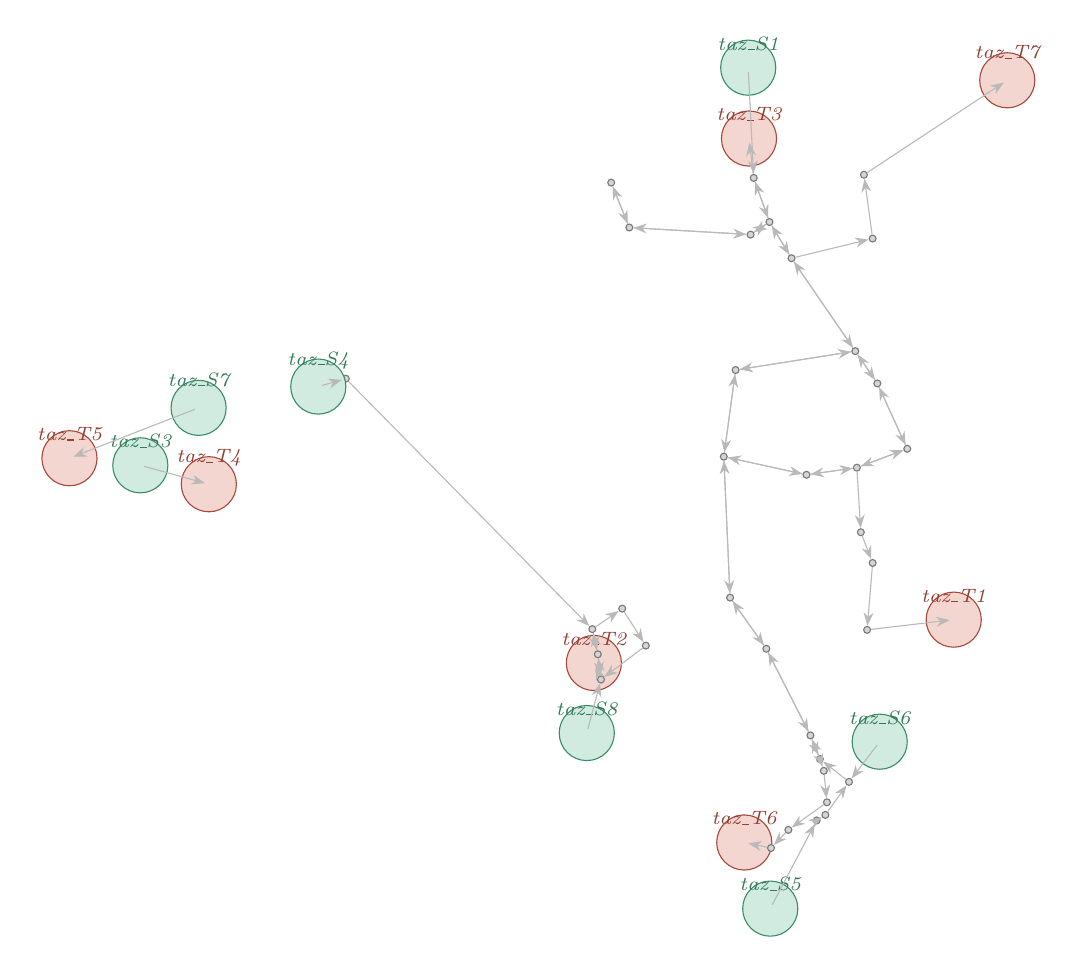
\begin{tikzpicture}[
    >=Stealth,
    inode/.style = {circle, draw=intcolor!80!black, fill=intcolor!40, inner sep=0pt, minimum size=2.5pt},
    onode/.style = {circle, draw=origincolor!80!black, fill=origincolor!25, minimum size=7mm, font=\tiny\bfseries, inner sep=0pt},
    dnode/.style = {circle, draw=destcolor!80!black, fill=destcolor!25, minimum size=7mm, font=\tiny\bfseries, inner sep=0pt},
    roadedge/.style = {->, thin, gray!55, shorten >=1.5pt, shorten <=1.5pt},
    onodelabel/.style = {font=\scriptsize\itshape, text=origincolor!70!black},
    dnodelabel/.style = {font=\scriptsize\itshape, text=destcolor!70!black},
]

% -- nodes --
\node[inode] at (6.79,8.86) {};
\node[onode] (n14922) at (10.20,1.76) {};
\node[onodelabel, above=1mm] at (10.20,1.76) {taz\_S6};
\node[dnode] (n70496) at (6.57,2.76) {};
\node[dnodelabel, above=1mm] at (6.57,2.76) {taz\_T2};
\node[inode] at (6.93,3.45) {};
\node[inode] at (7.23,2.98) {};
\node[dnode] (n72506) at (1.68,5.03) {};
\node[dnodelabel, above=1mm] at (1.68,5.03) {taz\_T4};
\node[inode] at (10.17,6.31) {};
\node[inode] at (10.55,5.48) {};
\node[inode] at (9.08,7.90) {};
\node[inode] at (8.60,8.92) {};
\node[inode] at (3.42,6.37) {};
\node[inode] at (8.56,8.20) {};
\node[inode] at (8.80,8.36) {};
\node[onode] (n14914) at (3.07,6.27) {};
\node[onodelabel, above=1mm] at (3.07,6.27) {taz\_S4};
\node[inode] at (9.04,0.64) {};
\node[inode] at (9.40,0.76) {};
\node[inode] at (7.02,8.29) {};
\node[dnode] (n26417) at (11.14,3.31) {};
\node[dnodelabel, above=1mm] at (11.14,3.31) {taz\_T1};
\node[inode] at (9.27,5.15) {};
\node[inode] at (9.96,4.42) {};
\node[inode] at (9.91,5.24) {};
\node[inode] at (10.11,4.03) {};
\node[inode] at (8.37,6.48) {};
\node[inode] at (9.89,6.72) {};
\node[inode] at (8.76,2.94) {};
\node[inode] at (9.32,1.84) {};
\node[inode] at (8.30,3.59) {};
\node[onode] (n61001) at (8.53,10.32) {};
\node[onodelabel, above=1mm] at (8.53,10.32) {taz\_S1};
\node[inode] at (10.00,8.96) {};
\node[inode] at (9.53,0.99) {};
\node[inode] at (9.49,1.39) {};
\node[inode] at (10.04,3.18) {};
\node[inode] at (9.51,0.83) {};
\node[inode] at (9.44,1.54) {};
\node[onode] (n20175) at (8.81,-0.36) {};
\node[onodelabel, above=1mm] at (8.81,-0.36) {taz\_S5};
\node[dnode] (n6274) at (8.48,0.48) {};
\node[dnodelabel, above=1mm] at (8.48,0.48) {taz\_T6};
\node[inode] at (6.62,2.87) {};
\node[dnode] (n59493) at (11.82,10.16) {};
\node[dnodelabel, above=1mm] at (11.82,10.16) {taz\_T7};
\node[inode] at (10.11,8.15) {};
\node[dnode] (n23995) at (-0.09,5.36) {};
\node[dnodelabel, above=1mm] at (-0.09,5.36) {taz\_T5};
\node[onode] (n40637) at (1.55,6.00) {};
\node[onodelabel, above=1mm] at (1.55,6.00) {taz\_S7};
\node[inode] at (8.82,0.41) {};
\node[inode] at (6.55,3.19) {};
\node[inode] at (6.66,2.55) {};
\node[onode] (n61435) at (6.48,1.87) {};
\node[onodelabel, above=1mm] at (6.48,1.87) {taz\_S8};
\node[inode] at (8.22,5.38) {};
\node[inode] at (9.81,1.25) {};
\node[onode] (n1185) at (0.81,5.27) {};
\node[onodelabel, above=1mm] at (0.81,5.27) {taz\_S3};
\node[dnode] (n47680) at (8.54,9.42) {};
\node[dnodelabel, above=1mm] at (8.54,9.42) {taz\_T3};

% -- edges (real directed street segments, L=66) --
\draw[roadedge] (10.17,6.31) -- (10.55,5.48);
\draw[roadedge] (6.62,2.87) -- (6.66,2.55);
\draw[roadedge] (6.55,3.19) -- (6.62,2.87);
\draw[roadedge] (8.60,8.92) -- (8.80,8.36);
\draw[roadedge] (8.53,10.32) -- (8.60,8.92);
\draw[roadedge] (9.32,1.84) -- (9.44,1.54);
\draw[roadedge] (8.76,2.94) -- (9.32,1.84);
\draw[roadedge] (8.30,3.59) -- (8.76,2.94);
\draw[roadedge] (3.42,6.37) -- (6.55,3.19);
\draw[roadedge] (6.79,8.86) -- (7.02,8.29);
\draw[roadedge] (9.89,6.72) -- (8.37,6.48);
\draw[roadedge] (9.08,7.90) -- (10.11,8.15);
\draw[roadedge] (8.56,8.20) -- (7.02,8.29);
\draw[roadedge] (8.22,5.38) -- (8.30,3.59);
\draw[roadedge] (8.37,6.48) -- (8.22,5.38);
\draw[roadedge] (8.80,8.36) -- (8.56,8.20);
\draw[roadedge] (9.91,5.24) -- (10.55,5.48);
\draw[roadedge] (9.27,5.15) -- (9.91,5.24);
\draw[roadedge] (8.22,5.38) -- (9.27,5.15);
\draw[roadedge] (9.89,6.72) -- (10.17,6.31);
\draw[roadedge] (9.08,7.90) -- (9.89,6.72);
\draw[roadedge] (8.80,8.36) -- (9.08,7.90);
\draw[roadedge] (10.11,8.15) -- (10.00,8.96);
\draw[roadedge] (10.55,5.48) -- (10.17,6.31);
\draw[roadedge] (6.66,2.55) -- (6.62,2.87);
\draw[roadedge] (6.62,2.87) -- (6.55,3.19);
\draw[roadedge] (8.80,8.36) -- (8.60,8.92);
\draw[roadedge] (8.60,8.92) -- (8.54,9.42);
\draw[roadedge] (6.93,3.45) -- (7.23,2.98);
\draw[roadedge] (7.23,2.98) -- (6.66,2.55);
\draw[roadedge] (9.44,1.54) -- (9.32,1.84);
\draw[roadedge] (9.32,1.84) -- (8.76,2.94);
\draw[roadedge] (8.76,2.94) -- (8.30,3.59);
\draw[roadedge] (10.04,3.18) -- (11.14,3.31);
\draw[roadedge] (3.07,6.27) -- (3.42,6.37);
\draw[roadedge] (7.02,8.29) -- (6.79,8.86);
\draw[roadedge] (8.37,6.48) -- (9.89,6.72);
\draw[roadedge] (9.91,5.24) -- (9.96,4.42);
\draw[roadedge] (9.96,4.42) -- (10.11,4.03);
\draw[roadedge] (10.11,4.03) -- (10.04,3.18);
\draw[roadedge] (9.81,1.25) -- (9.44,1.54);
\draw[roadedge] (7.02,8.29) -- (8.56,8.20);
\draw[roadedge] (9.04,0.64) -- (8.82,0.41);
\draw[roadedge] (9.51,0.83) -- (9.81,1.25);
\draw[roadedge] (9.40,0.76) -- (9.51,0.83);
\draw[roadedge] (10.20,1.76) -- (9.81,1.25);
\draw[roadedge] (8.30,3.59) -- (8.22,5.38);
\draw[roadedge] (8.22,5.38) -- (8.37,6.48);
\draw[roadedge] (8.56,8.20) -- (8.80,8.36);
\draw[roadedge] (6.48,1.87) -- (6.66,2.55);
\draw[roadedge] (10.55,5.48) -- (9.91,5.24);
\draw[roadedge] (9.91,5.24) -- (9.27,5.15);
\draw[roadedge] (9.27,5.15) -- (8.22,5.38);
\draw[roadedge] (10.17,6.31) -- (9.89,6.72);
\draw[roadedge] (9.89,6.72) -- (9.08,7.90);
\draw[roadedge] (9.08,7.90) -- (8.80,8.36);
\draw[roadedge] (9.44,1.54) -- (9.49,1.39);
\draw[roadedge] (9.49,1.39) -- (9.53,0.99);
\draw[roadedge] (8.81,-0.36) -- (9.40,0.76);
\draw[roadedge] (10.00,8.96) -- (11.82,10.16);
\draw[roadedge] (6.66,2.55) -- (6.57,2.76);
\draw[roadedge] (6.55,3.19) -- (6.93,3.45);
\draw[roadedge] (0.81,5.27) -- (1.68,5.03);
\draw[roadedge] (1.55,6.00) -- (-0.09,5.36);
\draw[roadedge] (9.53,0.99) -- (9.04,0.64);
\draw[roadedge] (8.82,0.41) -- (8.48,0.48);

\end{tikzpicture}%
}
\caption{Real-world sub-network (\texttt{intas\_crop}), cropped from the
InTAS (Ingolstadt) SUMO scenario~\parencite{lobo2020intas}. Green nodes are
origin TAZs, red nodes are destination TAZs, small gray dots are interior
junctions (unlabeled due to density -- real intersections have no natural
short names the way synthetic grid junctions do). Edges shown are the
$L=66$ monitored/routable edges only, i.e.\ the union of all enumerated
routes, not the full crop's road mesh; the true street layout is
considerably denser.}
\label{fig:network-intas-crop}
\end{figure}

\subsubsection*{Route structure}

Route enumeration identified $8$ candidate source TAZs and $7$ candidate
sink TAZs from the crop's boundary cut-points. Of the $8\times7=56$
possible source--sink combinations, $16$ are connected by at least one
legal route after the length and turning-restriction filters (source
\texttt{taz\_S2} has no legal route to any sink within the crop and is
therefore not part of the calibration setup, despite being a valid TAZ
definition). Ten of the $16$ OD pairs have two genuine alternative routes
(real detours through the street grid, not artificially constructed);
the remaining six are served by a single dedicated route. This gives
$D=16$ OD pairs and $R=26$ routes in total.

\subsubsection*{Edge-flow groups}

Unlike the synthetic networks, no edge grouping is applied: each of the
$L=66$ routable edges is its own flow variable, matching real SUMO edge
IDs directly (e.g.\ \texttt{32009827}, \texttt{-152077572\#2}). Because
these are real OSM-derived edges rather than hand-designed corridor
segments, edge lengths, lane counts, and speeds vary considerably across
the network, unlike the uniform edges of the synthetic grids.

\end{document}
